% Style Guide
% - use British English, exceptions: stroller vs buggy or pram, sidewalk vs pavement
% - active voice is preferred over passive voice, minimize passive
% - use past tense to describe what we did
% - try to avoid subsub sections (keep to two layers)
% - use siunitx for all units, surround with brackets [\si{\meter}], note the
%   common definitions, e.g. \si{\kph}
% - use tilde ~ to prevent line breaks in words that should stay together, e.g.
%   something~\cite{} or ISO~2631-1
% - only use "significant" when referring to statistical significance
% - use "infant", not "baby"
% - use "bicycle" instead of "bike"
% - use "amplitude spectrum/spectra" for what we plot
% - use "standard" not "norm"
% - use the oxford comma
% - TODO: acceleration vs accelerations ?
% - Data breakdown terms are "Session", "Trial" (of specific "Scenario"),
%   "Repetition"
% -  Referencing: Figure~\ref{fig:name}, Equation~\ref{eq:name},
%    Section~\ref{sec:name}, Appendix~\ref{app:name}, Table~\ref{tab:name}
% - inline urls \href{https://www.e.com}{my hyperlink}
% - do not use [h] for figures except in appendix, let latex place them where it
%   wants
% - figures should be 300 dpi and sized to the actual physical dimension in the
%   paper
% Other Notes
% - be careful about editing autogenerated tables, they will be overwritten

\documentclass[a4paper]{article}

\usepackage{amsmath}  % extra math features
\usepackage{booktabs}  % nice tables
\usepackage[margin=25mm]{geometry}
\usepackage{graphicx} % required for inserting images
\usepackage{hyperref} % clickable hyperlinks
\usepackage{multirow}  % pandas to_latex() uses this
\usepackage{siunitx}  % use for all units
\usepackage{subcaption}  % for subfigures

% hyperref settings for better looking links
\hypersetup{
  colorlinks=true,
  linkcolor=blue,
  urlcolor=blue,
  citecolor=blue,
}

% NOTE : Use as \si{\kph} or \si{\mps}
\def\kph{\kilo\meter\per\hour}
\def\mps{\meter\per\second}
    
\title{
  Vibration Characterisation of Strollers and\\
  Cargo Bicycles for Transporting Infants\\
  \vspace{2mm}
  \large{Including Recommendations for Users, Designers, Manufacturers, and Researchers} \\
  \vspace{2mm}
  \large{Prepared for VeiligheidNL}
}
% Gabriele as first, Jason as last, alphabetical for intermediate (discuss in meeting if other method desired
\author{
Gabriele Dell'Orto \and
Brecht Daams \and
Riender Happee \and
Georgios Papaioannou \and
Arjo J. Loeve \and
Jesper Meijerink \and
Thomas Valk \and
Jason K. Moore
}

\begin{document}

\maketitle

\color{red}
\section*{\centering Notice}
%
This report or its findings may not be shared outside of VeiligheidNL and
TU~Delft without further review of the methods and findings.
We also need to carefully consider possible adverse effects of dissemination. In
particular we need to consider:
%
\begin{itemize}
  \item System manufacturers being negatively affected by publication.
    Organisations like Consumentenbond typically give manufacturers access to
    draft test results, and give an opportunity to react. We can do this as
    well. We may now remove Brand and type information from this report. In a
    later stage we may test multiple products and then publish a comparison.
  \item Stimulating car use to transport infants and children. We don't want
    newspaper/online headlines which are overly alarming, and later turn out to
    be debatable.
\end{itemize}
\color{black}

\begin{abstract}
  Infants are transported in strollers and in baby seats mounted in cargo
  bicycles. The infants experience whole-body vibration during the associated
  walking and cycling trips, but there is little existing knowledge about
  associated comfort and health effects. To improve this, we measure the seat
  pan acceleration of five strollers and two styles of cargo bicycles with dummy
  infants representing ages 0 to 9 months over six different road surfaces of
  varying road roughness at typical travel speeds. The five strollers included
  three modern systems and two vintage systems with some level of suspension.
  One cargo bicycle had electric support enabling speeds up to 25~\si{\kph}. We
  report average seat pan acceleration for 78 different scenarios and
  investigate the effects of road surface, vehicle, seat type, and travel speed.
  Using the whole-body vibration ISO standards, we show that rough road
  surfaces, amplified by travel speed, may have health risks for travel
  durations as low as \SIrange{10}{30}{\min}. Stroller designs from 50 years ago
  significantly reduce vibrations, relative to most modern strollers we tested,
  indicating the need for return of suspension elements. Cargo bicycles ridden
  at the maximum electric bicycle speed over paver bricks can cause
  accelerations that should likely be avoided except for only the shortest of
  durations until more direct evidence of risks to infants is studied. Standards
  are needed for infant transport testing and evaluation, designers need to
  incorporate better suspension for infants, and research is needed to develop
  clear and direct connections to health and comfort effects.
\end{abstract}

\newpage

\tableofcontents

\newpage

\section{Introduction}
%Paragraph to introduce baby transport
When a baby is born, it is not able to walk. To move around or travel, it must
be either carried by adults or transported in a suitable means of wheeled
transport. Until about a century ago,  babies mainly stayed at home. This still
is customary in some non-Western cultures. A century ago, perambulators were
used to transport infants outdoors. However, mothers were advised that a playpen
in the garden is healthier than the use of a perambulator, partly because the
vibrations generated by a perambulator were deemed not comfortable and even
harmful for the baby~\cite{behrend1931}, even though in those days perambulators
had ample suspension. Since about 1970, cars became ubiquitous and the heavy and
sizeable perambulators became strollers: lighter and smaller products to enable
easy transportation in a car. Over the years, new means of transportation came
into use for infants: cars with a child car seat, bicycles with a bicycle seat
and cargo bicycles with either a car seat or a baby shell. 

%Paragraph to introduce baby vibration in transportation
All means of transport cause vibration, which is transferred to the infant
sitting or lying in it. Unlike the advice in the 1930s, vibration is seemingly
not a subject of attention in the present design of these products. On the
contrary, modern strollers do not have much suspension and cargo bicycles which
generate more vibration are increasingly used for infants. Interestingly, in the
literature we could find little about the maximal vibration load that babies and
older children can receive during transport without discomfort or harm, and
vibrations generated by infant transport are also only sparsely investigated.
Therefore the effect of transport on infant comfort and health can not easily be
assessed. To establish the amount of vibration that infants are subjected to in
transportation products, we investigated the vibration that infants receive
during transport in strollers and cargo bicycles. 

% Paragraph about motivation
Cycling, one of the active transportation modes, is advantageous for
health~\cite{Oja1998} and greatly contributes to reducing CO\(_2\) emissions,
congestion, and air pollution~\cite{Neves2019}. As a result, bicycles are
increasingly used as a means to deliver goods to consumers, and also for daily
commuting to work and personal matters (shopping, commuting with
children/infants, and others). Among all journeys in the EU, 20-40\% are by
bicycle or on foot, with bicycle trips most frequent in the Netherlands,
Denmark, and Sweden and less frequent in Finland. Various countries and
employers provide incentives to increase the use of bicycles. However, some
challenges need to be overcome to secure the wide acceptance and use of active
transportation modes. One of these challenges is the comfort levels experienced
by riders and passengers (i.e., infants/children in cargo bicycles), which is a
multifaceted aspect~\cite{ayachi2015identifying} and critical for the wide
acceptance and use of bicycles as a daily means of transport. Meanwhile, this is
a topic that is of great interest and requires attention when it comes to
infants' transportation with strollers or bicycles.

% Paragraph about comfort in bicycles
The research on cyclist comfort is a natural starting point for investigations
of similar road-induced vibrations for infants.
Comfort on bicycles~\cite{too1990biomechanics} is mainly affected by physical
comfort and the impact of environmental factors (weather, geometry of the route,
and road roughness).  
Physical comfort is related to mechanical (bicycle and component design),
biomechanical (whole-body vibrations, human body dynamics, and kinematics) and
physiological factors (individual characteristics, e.g. sex, body size, weight
and others).
While there is extensive literature exploring the impact of environmental
factors (i.e., irregular road surface quality, weather conditions) on cyclists'
comfort~\cite{Stinson2003,Hagemeister2003,ayachi2015identifying,Verhoeven2017,Teixeira2020},
there is limited work on understanding the biomechanical and physiological
factors of comfort while being carried by bicycle (infants/children in bicycle
seats, on cargo bicycles, or in trailers). A particular concern is the transport
of infants under one year, who cannot well express any experience of discomfort
or pain.
Similar concerns are raised when it comes to strollers, where infants are also
exposed to vibrations induced by roads. 
In this paper, we will explore biomechanical comfort by assessing the whole-body
vibrations that could be experienced by transported infants both in cargo
bicycles and strollers, and evaluating potential health risks and discomfort
that might arise.

% Paragraph about transmission of vibrations
Biomechanical comfort is mostly related to the vibrations induced by road
irregularities and transmitted via the vehicle to the human body and head while
being driven~\cite{too1990biomechanics}. 
According to the literature, road irregularities are a critical factor for the
amplitude of the resulting vibrations experienced by the bicyclists and
passengers, as the vibrations induced on the body and head are not efficiently
isolated due to the lack of or inadequate suspension systems in most of the
bicycle models~\cite{vasudevan2017comparison} or strollers.
The bicycle or stroller design and its specific configuration can affect the
sitting posture, and eventually the transmissibility of the
vibrations~\cite{Brand2020,Verma2016}.
The sitting posture can also vary in case of children/infants who may be
transported sitting or lying down in a different posture and location than the
cyclist (e.g. above a wheel when in a bicycle seat) and in/on a different `seat'
(a car seat, bicycle seat, stroller seat, or cot). 
These all influence the level of whole-body vibrations and the transmission of
the vibrations from the seat to the body and head.
Furthermore, the amplitude of the vibrations experienced by
bicyclists/passengers/transported infants while biking or being transported in a
stroller may increase because of increased travelling speed either due to
running with a stroller or due to the increased power offered by electric
bicycles (with and without trailers).
For the latter, the average speed of electric bicycles and speed pedelecs is
19\% higher (21.0~\si{\kph} and up to 63\% higher (28.1~\si{\kph}),
respectively, than the average speed of conventional bicycling~\cite{SWOV2022}.
The intensity of these vibrations could become even more critical with the
change of load, which could be related with age and size of the infant/children
transported. However, there is limited literature exploring the whole-body
vibrations of infants and children being transported by bicycles with trailers,
cargo bicycles, stroller seats and others
~\cite{Ota2012,Ota2014,Kanya-Forstner2020, vanDriessche2018,
Schwanitz2020,MalteChildComfort2022}.
At the same time, the available literature is mostly focusing on comfort rather
than health risks. 

% Paragraph about children in bicycles
One of the research fields closely related to vibrations acting on infants
during transportation is that of inflicted head injury by shaking trauma
(IHI-ST). However, there is a lack of reliable, applicable, validated injury
thresholds for assessing IHI-ST risks~\cite{hutchinson2024modeling}. Similarly,
even if there are significant indications that the vibration amplitude affects
comfort in bicycles or strollers, there are no standard assessment methods or
guidelines available with regards to their design. ISO~2631~\cite{ISO2631}, the
international standard for assessing whole-body vibrations, was derived using
datasets on motion platforms, adults as human participants and sitting postures
which are adopted in passenger vehicles rather than on bicycles.
This inconsistency was captured by Gao~et~al.~\cite{Gao2018}, who derived
different limits of comfort for adults riding on bicycles based on their
subjective feedback, compared to the vibration limits suggested by
ISO~2631-1.
In addition, the exposure time to the vibrations is not considered as a factor
of comfort by the ISO~2631-1, despite having a clear impact on health risks
according to the European Directive (2002/44/EC, 2002)
\cite{directive2002directive}.

% Paragraph Potential effects of vibrations on adults
Despite the lack of clarity with regards to comfort assessment or inflicted head
injury by shaking trauma for children/infants on bicycles, there are clear
indications in the literature that these should be explored and considered.
About 36\% of males and 42\% of females in a total sample of 900 people had
various complaints about comfort~\cite{groenendijk1992sitting}.
Discomfort for both men and women occurred even during short bicycle trips
(\SIrange{3}{10}{\kilo\meter}). However, results from research into comfort of
adult cyclists can not be applied directly to infants or children sitting or
lying in transportation systems.

Schwanitz~et~al.~\cite{Schwanitz2020} assessed accelerations in a child bicycle
trailer riding over smooth asphalt, gravel, and cobblestones using ISO~2631-1
weighted RMS vertical accelerations.
Anthropomorphic children shaped sandbag dummies (baby and toddler sizes) were
used as lumped masses. According to the results, tyre pressure and the number of
passengers had no significant effect on vibration magnitude, but road surface
and travel speed did. 
The baby sized dummy (5~\si{\kilo\gram}) experienced 20\% higher vibration than
the toddler sized dummy (10~\si{\kilo\gram}), while the measured values
generally exceeded the ISO~2631-1 vibrational comfort of adults.
Rothhämel~et~al.~\cite{MalteChildComfort2022} conducted measurements using a
trailer seat and a tadpole configuration three-wheel cargo bicycle on smooth
asphalt and cobblestones for speeds between \SIrange{10}{20}{\kph}. 
After weighting the accelerations using ISO~2631-1 methods, they found a large
increase of the vibration amplitude on cobblestones compared to asphalt on the
same speed range. The child trailer exhibited larger weighted RMS accelerations
than the cargo bicycle with the child seat between the front wheels. 
Both the trailer and cargo bicycle child seats had generally larger magnitude
vibrations than experienced in an automobile seat travelling at 30~\si{\kph} on
a rough road \cite{gromadowski2013analysis}. Rothhämel and
Liu~\cite{rothhamel2023comfort} conducted measurements with a
6.5~\si{\kilo\gram} mass representing an infant with various tyre pressures. All
their values fell into the ``extremely uncomfortable'' zone for the ISO~2631-1.

In addition to the studies with dummies or lumped masses representing
infants, Kanya-Forstner~\cite{Kanya-Forstner2020} measured acceleration in
bicycle child trailers with human subjects aged 12 months to 6 years over
asphalt and gravel terrain (averaged speed of 12~\si{\kph} over the
20~\si{\minute} ride). 
According to the health assessment using ISO~2631-1, the vibrations are similar
to the ones experienced in car seats in vehicles and illustrated moderate or low
health risk for a 2~\si{\hour} duration.
On the other hand, if not corrected for duration, the values point to moderate
and high risks. The terrain type had the greatest influence on vibration
exposure levels followed by trailer type, while gel cushions as support did not
significantly influence vibration measured at the seat/pan interface. Hence,
there is a need to re-focus on the impact of vibrations on infants and
children's health and comfort~\cite{rybarczyk2020physiological} to ensure the
safe, comfortable and wide use of bicycles. 

% Don't edit, working to change the following paragraph
In the context of infants transportation with stroller seats, Kok
Siong~\cite{lim2018study} carried out an indoor and an outdoor experiment to
capture the vibrations transmitted onto the seat and backrest of a baby
stroller, using weights from \SIrange{4}{14.14}{\kilo\gram}, and  a child
subject of 10.30~\si{\kilo\gram} as well as a dummy weighing
10.30~\si{\kilo\gram}. 
The comfort levels for the indoor testing were labelled as `Fairly
uncomfortable' to `A little uncomfortable', but the outdoor testing resulted in
`Extremely uncomfortable' and `Fairly uncomfortable' values. They used both a
child and dummy for the experiments, identifying similar patterns. However, the
results still consider ISO~2631-1 standard, which is designed for adults and
specific postures. In a similar research, Sierzputowski~
et~al.~\cite{sierzputowski2021pilot} investigated vibrations induced in a modern
and
an older stroller, when moving on different surfaces: asphalt road, concrete
paving blocks, concrete plates, dirt road, lawn and damaged concrete. The
obtained weighted RMS acceleration values based on ISO~2631-1 were several times
in the range of the highest discomfort (>2~\si{\mps\squared}). 
Another research which included also children as test subjects was conducted by
Okajima~et~al.~\cite{okajima2020dynamic} measuring vibrations that seven
children received, sitting upright in a stroller, when riding over a protrusion
(13x60 mm) with either one wheel or two wheels. 
The children were 3 to 6 years old, boys and girls, weighing
\SIrange{15.94}{19.96}{\kilo\gram} and measuring
\SIrange{98.0}{112.4}{\centi\meter} in length. 
Based on the results, the infant’s head and chest exhibit strong vibrations at
1~\si{\hertz} along all three axes (x,y and z), vibrate easily along the
y-direction at 2~\si{\hertz}, and are less likely to vibrate at more than
8~\si{\hertz}. 
This result is critical as this range of frequencies is very common in bicycles
and strollers. However, they did not assess the comfort and the health risk when
the children were exposed to these vibrations. 
Despite significant research on the effect of whole-body vibrations on
children's comfort, there is limited research on infants.

This paper reports on the vibration induced on infants of different ages when
transported in strollers and cargo bicycles. 
Vibration can be related to discomfort and might lead to negative health
consequences. However, the topic is poorly addressed in scientific literature,
and only a few studies focus on the effect of vibration on babies as reviewed
above. 
To measure the actual vibration transmitted to infants, we equipped five
strollers and two cargo bicycles with inertial measurement units (IMU) and
conducted 78 experiments on different road surfaces and travel speeds, using
dummies representing the size and mass of 0, 3, and 9 months old infants.
We present results in the time and frequency domains, which allows comparing
vertical accelerations at the baby-seat interface, as recommended by ISO~2631-1
standards for vibration discomfort.
We investigated the influence of different variables on vibration, such as type
of vehicle, baby seat, travelling speed, dummy size and mass, and road surfaces
and provide recommendations to users, designers, and future researchers based on
the findings.

\section{Methods}
%
\subsection{Test Equipment}
%
Vibration measurements were conducted at approximate constant speed using five
different strollers, two cargo bicycles, and two baby
seats~\footnote{Appendix~\ref{app:equipment} provides figures and technical
descriptions of all the strollers and cargo bicycles.}, chosen for their
popularity and/or distinctive features:

\begin{description}
\item[Strollers] A selection of vintage and modern strollers for carrying
infants. The modern strollers are configurable as cots for newborns and as seats
for older infants.
%
\begin{description}
  \item[Maxi-Cosi Street Plus] This stroller comes
  with a cot configuration (0-3 months) and an infant seat option. It has large wheels, with only a marginal suspension system.
  (\href{https://www.maxi-cosi.nl/kinderwagens/street-plus?color_swatch_id=5519}{Maxi-cosi website})
  \item[Stokke BABYZEN YOYO 0+] The smallest foldable stroller on the
  market. It has only a marginal suspension system and smaller wheels compared to those of other strollers available on the market.
  (\href{https://tinylibrary.nl/products/kinderwagen-babyzen-yoyo-0-plus}{Model
  rented for the experiment})
  \item[Bugaboo Fox 5] Featuring large wheels and a suspension system
  that makes it an all-terrain stroller according to the manufacturer. It has large puncture-proof tyres and an air-permeable mattress.
  (\href{https://www.bugaboo.com/nl-nl/speciale-aanbiedingen/bugaboo-fox-5-bassinet-and-seat-stroller-black-base-midnight-black-fabrics-midnight-black-sun-canopy-PV006272.html?gad_source=1&gclid=Cj0KCQiA1Km7BhC9ARIsAFZfEIuB-6fQPRl5KyIHVJtion5lyD_Z1Qn-IP3shWoB_HXFozM1ySTXNfgaAgzFEALw_wcB&gclsrc=aw.ds}{Bugaboo
  website})
  \item[Green Machine] An unknown brand vintage perambulator, dating
  approximately from the 1970's that includes a leather strap suspended cot in a
  metal frame. The wheels are relatively large in diameter compared to the
  modern strollers.
  \item[Old Rusty] An unknown brand vintage seat-style stroller from
  approximately the 1970's that includes a metal spring suspension system and
  wheels that are slightly larger than the modern strollers.
\end{description}
\item[Cargo Bicycles] Two modern Dutch ``bakfietsen'' in which different baby
seats can be mounted.
%
\begin{description}
  \item[Urban Arrow Bicycle] A popular electric cargo bicycle in The
  Netherlands. This vehicle has two inline wheels which makes it roll into
  curves like a regular bicycle. It is featured by a long frame that can carry
  loads (e.g. a child in a car seat or baby shell) placed in between the rider
  and the front wheel. 
  (\href{https://urbanarrow.com/}{Urban Arrow website})
  \item[Keiler Tricycle] A tadpole (two wheels in the front, one in the
  rear) cargo tricycle  without electric assist. This vehicle will not roll into
  curves. However, differing road surface unevenness at the left and right front
  wheel will induce lateral roll and lateral acceleration in infants. We added
  masses in specific locations to simulate the presence of an electric motor and
  battery package. (\href{https://kashop.nl/product/keiler-bakfiets/}{Product
  Webpage}) 
\end{description}
\item[Baby Seats] These two baby seats were mounted in the cargo bays of the two
cargo bicycles.
%
\begin{description}
  \item[Maxi-Cosi X Joolz Pebble Pro i-Size Car Seat] Can be adapted to be
  mounted on cargo bicycles with a fitting fixing system (e.g. ``Urban Arrow
  Baby Car Seat Adapter''). Comes with an integrated suspension system. The same
  adapter was used in both cargo bicycles.
    (\href{https://www.maxi-cosi.nl/autostoelen/pebble-pro-i-size}{Maxi-Cosi
    Webpage})
  \item[Melia Baby Shell] Baby seat specifically designed for cargo bicycles
  meant for babies from 2 to 9 months old. Mounted to the seat platform in both
  cargo bicycles.
    (\href{https://melia.nl/product/babyschaal-4-seizoenen-comfort/}{Melia
    Webpage})
\end{description}
\end{description}

The tests involved three baby dummies with sizes and weights representative of
newborns and 3 and 9 month old infants. Newborns (`0 months') are the youngest
(smallest, lightest) children that are transported in strollers with a cot.
Three month old infants are the youngest (smallest, lightest) children that are
transported in cargo bicycles, fixated in a baby car seat or baby shell. Nine
month old infants are the youngest (smallest, lightest) that can sit up straight
by themselves and thus can be transported sitting up straight, in a stroller
with a seat or on the bench of a cargo bicycle.

We considered the use of ``crash test dummies'' (also known as anthropomorphic
test devices or ATD's) which are designed and commonly used to test child seats
in car crash tests. However, the nearest available body sizes for crash test
dummies were a 6-weeks Q0-dummy, a 6-months Crabi dummy, and a 12-months Q-dummy
(Humanetics, Farmington Hills, USA). These 3 dummies are of a fundamentally
different design, hampering comparison, and did not match the desired body
sizes. Moreover, these child dummies have dynamic properties designed for crash
conditions, and they were designed based on scaling of adult biomechanical data
rather than child data, so in that respect there is no benefit over other
dummies. 

Testing with real infants would be unethical, and would create challenges in
terms of reproducibility. Hence we bought and adapted ``reborn'' dummies
available in a wide range of postures from a webshop specialising in dolls and
dummies (\href{http://www.atelier-wiesje.nl}{Atelier Wiesje}). The dummies were
filled with a mixture of cat litter sand and water to reproduce the exact
weights needed for testing. Cat litter sand features smooth and round-shaped
grains, which do not damage the dummies' materials (fabric and plastic). The
weight and body height of the dummies were made to match the average measures
for children of 0, 3 and 9 months old.

We wanted to use the measurements from Steenbekkers~\cite{Steenbekkers1993}.
However, this research provided the results only per three-month group, which
did not fit our age categories. We decided to use the growth charts used by
clinicians to assess infant growth to determine the average weight and body
height at the right ages. The average weight at 0 months and the average body
height at all three ages are derived from Dutch growth charts. We used
measurements of Dutch children because they are the target group of the project
funder, VeiligheidNL. Dutch children are also the tallest in Europe. We derived
the average weight of 3 and 9 months old children from French growth charts.
French children are the smallest in Europe. At 3 months, average Dutch children
weigh 113 gram more than average French children and at 9 months, the difference
is 85 gram. The following lists the dummies used:
%
\begin{description}
  \item[Dummy 0 months] weight 3.48~\si{\kg}, size 50~\si{\cm}. Dollkit 20'',
  ``Andi Asleep'' (product code AW380008).
  (\href{http://www.atelier-wiesje.nl/index.php?item=9912---dollkit-20-_-andi-asleep--_-armen-_-_-benen----available&action=article&group_id=10000164&aid=2163&lang=NL}{Webpage})
  
  \item[Dummy 3 months] weight 5.90~\si{\kg}, size 62.5~\si{\cm}. Dollkit 25'',
  ``Asia - Limited Edition'' (product code 300287).
  (\href{http://www.atelier-wiesje.nl/index.php?action=article&aid=2556&group_id=10000176&lang=NL}{Webpage})
  \item[Dummy 9 months] weight 8.90~\si{\kg}. Size 70~\si{\cm}. Dollkit 28'',
  ``Hailey'' (product code 304137).
  (\href{http://www.atelier-wiesje.nl/index.php?action=article&aid=1974&group_id=10000133&lang=NL}{Webpage})
\end{description}

To achieve a realistic mass distribution in the body of the dummies, each limb
was filled with a proper amount of wet sand (for the 0-month dummy, water was
added to achieve the correct weight). To do this, we simplified the geometry of
each body segment according to the defined basic geometric shapes: a sphere for
the head, and cylinders for the torso, upper arms, upper legs and lower legs,
according to what was stated in~\cite{Snyder1977}. We also assumed an equal
density for each limb, and we rescaled the measurements of the limb segments
reported in \cite{Snyder1977} to match the dimensions of our dummies. In doing
so, we were able to calculate the volume of each segment, thus the mass of each
limb of the dummies (assuming a density of 1000~\si{\kg\per\cubic\meter}).

\subsection{Measurement Equipment}
%
Linear accelerations and angular velocities were measured tri-axially using
Consensys Shimmer3 IMUs with a Consensys Base 6U.01 dock (Shimmen Sensing,
Dublin, Ireland). The IMUs were updated to firmware version LogAndStream v0.11.0
and managed via the software ConsensysBASIC v1.6.0-64bit on a Dell 7310 laptop
with Microsoft Windows 10. We 3D printed supports (material: PLA) for the
sensors to ensure a firm clamp between the sensor and the bicycle/stroller
tested (Small white and orange boxes visible in Figure~\ref{fig:sensors_UA}).
Each vehicle was equipped with five IMUs, as listed below. All the drawings
showing the vehicles and the sensors' location are reported in
Appendix~\ref{app:equipment}.
%
\begin{enumerate}
  \item \textbf{Rear Wheel} This IMU was placed on the wheel hub (cargo
  bicycles) or clamped to the wheel (strollers) for measuring the travel speed.
  The travelling (longitudinal) speed was derived according to:
  %
  \begin{align}
    v = \omega \cdot r
    \label{eq:long-speed}
  \end{align}
  %
  where \(\omega\) is the angular speed of the wheel (obtained from the IMU's
  gyroscope aligned with the wheel's axis) and \(r\) is the radius of the wheel.
  \item \textbf{Front Wheel} This IMU was mounted on the front wheel fork (the
  caster wheel for the stroller). This was the non-rotating measurement point
  closest to the ground. The purpose of this sensor was to measure the road
  roughness filtered out only by the tyres.  
  \item \textbf{Frame} On the cargo bicycle, an IMU was placed below the frontal
  cargo bay and clamped to the frame. This was to provide an understanding of
  the damping characteristics of the bicycle frame, together with an estimation
  of the effect of the suspension system. On the stroller, the IMU was taped
  under the baby seat.
  \item \textbf{Seat Head} IMU taped into the baby seat (on the soft mattress),
  directly in contact with the dummy's head. This IMU measured the vibration
  transmitted to the head contact point.
  \item \textbf{Seat Pan} This IMU was taped into the baby seat, at the
  interface between the dummy's buttock and the baby seat. It measured the
  vibration transmitted to the dummy's buttock.
\end{enumerate}

\begin{figure}
  \centering
  \subcaptionbox{IMU on the front fork}{\includegraphics[width=0.45\textwidth, angle=-90]{fig/FW_UA.jpg}}
  \subcaptionbox{IMU on the rear wheel hub}{\includegraphics[width=0.45\textwidth, angle=-90]{fig/RW_UA.jpg}}
  \subcaptionbox{IMU under the cargo bay}{\includegraphics[width=0.45\textwidth, angle=-90]{fig/BT_UA.jpg}}
  \subcaptionbox{IMUs on the baby seat surface}{\includegraphics[width=0.45\textwidth, angle=-90]{fig/Maxicosi_sensors_UA.jpg}}
  \caption{IMU locations on the Urban Arrow cargo bicycle. The white 3D printed
  sensor supports are visible in (a) and (c). The last figure (d) shows how the
  sensors were taped to the seat pan and backrest.}
  \label{fig:sensors_UA}
\end{figure}

The IMUs for the seat head and seat buttock positions contacting the dummy were
placed according to the recommended practice in vibration testing standard
ISO-2631-1. This generates acceleration data representative of the mechanical
load transferred from the seat to the human body taking into account the
compliance of the seat foams and the inertia and compliance of the dummy. 

The target sampling frequency was 910.22~\si{\hertz} for all IMUs. The
full-scale range was set to \(\pm\)16~g for the accelerometer (``WR: wide
range'' configuration on Consensys Shimmer software), and
\(\pm\)2000~\si{\degree\per\second} for the gyroscope. All tests were recorded
with two GoPro Hero7 cameras: one directly mounted on the strollers/bicycles to
record the dummy-seat relative motion, while the other was held by an
experimenter walking or riding alongside the vehicle to have a complete overview
of the experiment.

\subsection{Experimental Protocol}
%
All tests were conducted in Delft, The Netherlands, on public roads near the
Delft University of Technology, Faculty of Mechanical Engineering. Latitude and
longitude of each location along with local photographs of each site are
provided in Appendix~\ref{app:location}.
After mounting the sensors and reaching the location of the experiment, we
turned on the sensors to start the experimental session. Before each trial, we
pushed the vehicle back and forth on level ground to mark the beginning of the
trial as an extra time-synchronization measure.
For the cargo bicycle test, a single rider conducted all trials to be consistent
across different sessions (rider mass: 59~\si{\kg}; rider height:
1.70~\si{\m}).
We tested three types of road surfaces with the cargo bicycles and repeated
those at different speeds.
The stroller tests were conducted on six different surfaces with the pusher
manually keeping a consistent walking speed of approximately
5~\si{\kilo\meter\per\hour}.
In all tests, speed was controlled by the pusher or cyclist using a speedometer
mounted on the stroller handle bar or the steer of the cargo bicycle. We
gathered data from multiple trials within the same session. The test
combinations, ``scenarios'', are listed below.
%
\begin{itemize}
  \item \textbf{Strollers}  The stroller tests were done with the dummies of 0
  months and 9 months old. All the test surfaces listed below are shown in
  Appendix~\ref{app:location}.
  \begin{itemize}
      \item Tarmac
      \item Paver bricks % Klinkers
      \item Sidewalk pavers % Stoeptegels
      \item Cobblestones 
      \item Sidewalk slabs (concrete blocks with gaps in between) % Aula blocks
      \item Shock bump: A 30x30~\si{\mm} square section aluminium bar was taped
      to the ground (smooth surface)
  \end{itemize}
  \item \textbf{Cargo bicycles} The cargo bicycle tests were conducted using the
  dummies of 0 months and 3 months. With the Keiler tricycle, the speed was
  limited to 20~\si{\km\per\hour} for safety reasons (due to wobbling), and
  difficulties to safely keep a constant speed over 22~\si{\km\per\hour}. The
  test surfaces are listed below:
  \begin{itemize}
      \item Tarmac
      \item Paver bricks
      \item Shock bump: As mentioned before, we conducted shock test riding over
      a 30x30~\si{\mm} square section aluminium bar, at three speeds: 
      \begin{itemize}
          \item Low speed: 5~\si{\kph}
          \item Medium speed: 12~\si{\kph}
          \item High speed: 20~\si{\kph} for the Keiler tricycle,
          25~\si{\kph} for the Urban Arrow cargo bicycle
      \end{itemize}
  \end{itemize}
  \item \textbf{Baby seats} Both the Maxi-Cosi X Joolz Pebble Pro i-Size and the
  Melia baby shell were tested on each cargo bicycle using the same mounting
  systems.
\end{itemize}

\subsection{Postures}
%
All tested systems provided full support of back and head and allowed usage in
lying or at least reclined postures. Nine month old infants would be able to sit
erect but will often rest their heads or be asleep. Although sitting upright is
the best posture for children who can sit upright, a more reclined posture was
tested because this allowed measurement of vibration at the head-seat interface
while the head was always supported by the headrest. We tested all systems with
horizontal or reclined postures. The inclination angle with respect to the
ground is listed in Table~\ref{tab:baby-posture} for each condition tested.
%
\begin{table}
  \centering
  \caption{Inclination angles of the IMUs ``Seat Head'' and ``Seat Pan'', per
  each tested configuration. We report the angles defined by the axis of the
  human body reference system (a reference system connected to the dummy, whose
  z-axis is aligned with the body spine and x-axis points to the front of the
  body) and the ground plane. An angle 90~\si{\degree} indicates supine posture,
  -90~\si{\degree} indicates recumbent posture, and 0~\si{\degree} means erect
  posture.}
\begin{tabular}{lllrrr}
\toprule
 &  &  & & \multicolumn{2}{c}{Inclination angle [deg]}  \\
Vehicle Type & Model & Dummy & Baby seat & Seat Head & Seat Pan\\
\midrule
\multirow[t]{6}{*}{Cargo Bicycle} & \multirow[t]{3}{*}{Urban Arrow} & 0 mo & Maxi-Cosi X Joolz & 49
& -43 \\
 &  & 3 mo & Maxi-Cosi X Joolz & 49 & -43 \\
 &  & 3 mo & Melia & 26 & -28 \\
\cline{2-6}
 & \multirow[t]{3}{*}{Keiler} & 0 mo & Maxi-Cosi X Joolz & 49 & -43 \\
 &  & 3 mo & Maxi-Cosi X Joolz & 49 & -43 \\
 &  & 3 mo & Melia & 26 & -28 \\
\cline{1-6} \cline{2-6}
\multirow[t]{5}{*}{Stroller} & Maxi-Cosi Street Plus & 0 mo & Baby cot & 90 & 90\\
\cline{2-6}
 & Maxi-Cosi Street Plus & 9 mo & Baby seat & 50 & -40 \\
\cline{2-6}
 & Babyzen YOYO 0+ & 0 mo & Baby cot & 78 & 78 \\
\cline{2-6}
& Babyzen YOYO 0+ & 9 mo & Baby seat & 45 & -41 \\
\cline{2-6}
& Bugaboo Fox 5 & 0 mo & Baby cot & 90 & 90 \\
\cline{2-6}
 & Bugaboo Fox 5 & 9 mo & Baby seat & 41 & -24\\
\bottomrule
\end{tabular}
  \label{tab:baby-posture}
\end{table}

\subsection{Data Processing}
% 
We analysed the raw data with a custom data processing pipeline. The pipeline's
open source code (MIT license) is hosted at
\href{https://github.com/mechmotum/baby-vibration}{github.com/mechmotum/baby-vibration}
implemented in Python 3.13.1 using the following software packages:
DynamicistToolKit 0.6.1, Matplotlib 3.9.3, NumPy 2.2.0, Pandas 2.2.3, pyyaml
6.0.2, SciPy 1.14.1, Seaborn 0.13.2, and statsmodels 0.14.4. The pipeline
generates a website at
\href{https://mechmotum.github.io/baby-vibration}{mechmotum.github.io/baby-vibration} with an exhaustive collection of figures for examining the
quality of the data and general results for all trials including the selected
tables and figures presented and discussed in the results section of this paper.

We define a ``session'' as a continuous data collection period from a single
vehicle. Each session is segmented into ``trials'' corresponding to a different
road surface or activity and each trial is divided into subsequent, back-to-back
``repetitions''.
The raw data consists of a single comma-separated value (CSV) file per session
per IMU along with metadata for the sessions and vehicles. The CSV file contains
the time series data from each IMU: linear acceleration along and angular speed
about each of the body-fixed orthogonal axes of the IMU alongside Epoch Unix
timestamps. We segment the sessions into trials representing a motion state of
the vehicle: either static on level ground or being propelled over one of the
surfaces of interest at a constant speed. Figure~\ref{fig:session} gives an
example of segmenting a session in different trials. The data were processed per
session as follows:
%
\begin{enumerate}
  \item Calculate the vehicle travel speed during the session from the angular
    rate of the rear wheel and the vehicle's wheel radius.
  \item Extract segments representing a single trial from each session time
    history, based on the manually labelled segment ``start'' and ``end'' times.
  \item Split the trials with durations longer than 40~\si{\second} into
    repetitions of \SIrange{20}{39}{\second}.
  \item Rotate the accelerometer data for each sensor from body-fixed sensor
    coordinates to body-fixed vehicle coordinates and subtract the constant
    standard gravity component. This is achieved by rotating the coordinate axes
    about the sensor's body-fixed axis which was manually aligned with the
    vehicle's pitch axis. We subtracted the mean measured acceleration due to
    gravity giving linear acceleration of each sensor projected into the
    vehicle's SAE body-fixed axes~\cite{SocietyofAutomotiveEngineers2008},
    named: longitudinal $x$, lateral $y$, and vertical $z$.
  \item Extract each motion trial segment and select the vehicle body-fixed
    longitudinal, lateral, and vertical component of the seat pan accelerometer.
\end{enumerate}
%
This resulted in acceleration-time recordings of 220 total repetitions. The
non-shock repetitions have durations in the range of \SIrange{10}{40}{\second}
(mean: 25~\si{\second}), see Table~\ref{tab:num-trials} for a breakdown of the
non-shock repetitions.
%
\begin{figure}
  \centering
  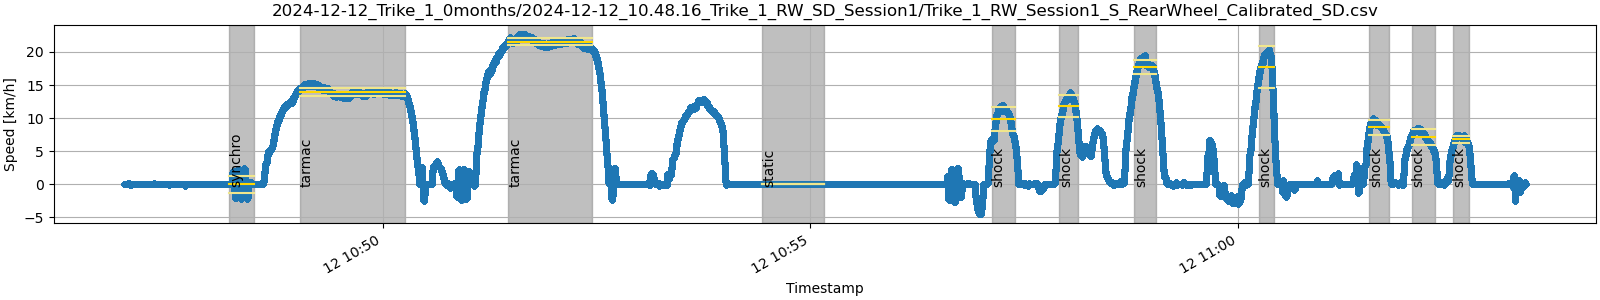
\includegraphics[width=160mm]{fig/session015.png}
  \caption{Vehicle speed versus time for an entire session (015) showing the
  trials in the shaded grey areas. Gold horizontal lines depict the mean speed
  during the trial bounded by the standard deviation of the speed.}
  \label{fig:session}
\end{figure}
%
% NOTE : This table is autogenerated from the data pipeline scripts and pasted in. I move the units to a second row manually for width conservation.
\begin{table}
  \centering
  \caption{Number of repetitions performed on each road surface, excluding
  shock, and speed along with the mean duration in seconds and its standard
  deviation.}
\begin{tabular}{llcccc}
\toprule
 &  &  & \multicolumn{2}{c}{Repetitions}\\
 &  & Target Speed & Count & Mean Duration & STD Duration \\
Vehicle Type & Road Surface & [\si{\kph}] & & [\si{\second}] & [\si{\second}] \\
\midrule
\multirow[t]{6}{*}{Cargo Bicycle} & \multirow[t]{3}{*}{Paver Bricks} & 12 & 13 & 25.1 & 7.0 \\
 &  & 20 & 8 & 28.8 & 7.6 \\
 &  & 25 & 3 & 33.4 & 4.3 \\
\cline{2-6}
 & \multirow[t]{3}{*}{Tarmac} & 12 & 14 & 25.0 & 7.0 \\
 &  & 20 & 6 & 25.2 & 7.2 \\
 &  & 25 & 6 & 22.0 & 2.5 \\
\cline{1-6} \cline{2-6}
\multirow[t]{5}{*}{Stroller} & Cobblestones & 5 & 26 & 22.8 & 5.6 \\
\cline{2-6}
 & Paver Bricks & 5 & 20 & 25.0 & 7.6 \\
\cline{2-6}
 & Sidewalk Pavers & 5 & 19 & 25.2 & 8.2 \\
\cline{2-6}
 & Sidewalk Slabs & 5 & 23 & 22.8 & 3.4 \\
\cline{2-6}
 & Tarmac & 5 & 16 & 28.9 & 9.6 \\
\cline{1-6} \cline{2-6}
 & & \textbf{Count Sum} & \textbf{154} & & \\
\bottomrule
\end{tabular}
  \label{tab:num-trials}
\end{table}

\subsection{Trial Analyses}
%
Figure~\ref{fig:vert-acc-example} shows an example time history of the vertical
acceleration of the seat pan during a single repetition. To perform the
ISO~2631-1 recommended health and comfort analysis, we first downsampled the
time history from the hardware-set variable sampling frequency of approximately
910.22~\si{\hertz} to a constant sample rate of 400~\si{\hertz} using linear
interpolation, giving sufficient samples for the bandwidth of interest based on
the Nyquist frequency. We set any acceleration values outside of the sensor
manufacturer's reported operating range of \(\pm\)16~g to that maximum or
minimum, respectively, given that values outside the range may be unreliable.
Values that exceed the range are rare and only present in some of the cargo
bicycle paver brick trials, but are common in the shock tests. Following the
ISO~2631-1 recommendation, we low-pass filtered the signal at
\(1.5\times80~\si{\hertz}=120~\si{\hertz}\) using a zero-lag
2\textsuperscript{nd} order Butterworth filter, given that the standard only
applies to frequencies up to 80~\si{\hertz}.
%
\begin{figure}
  \centering
  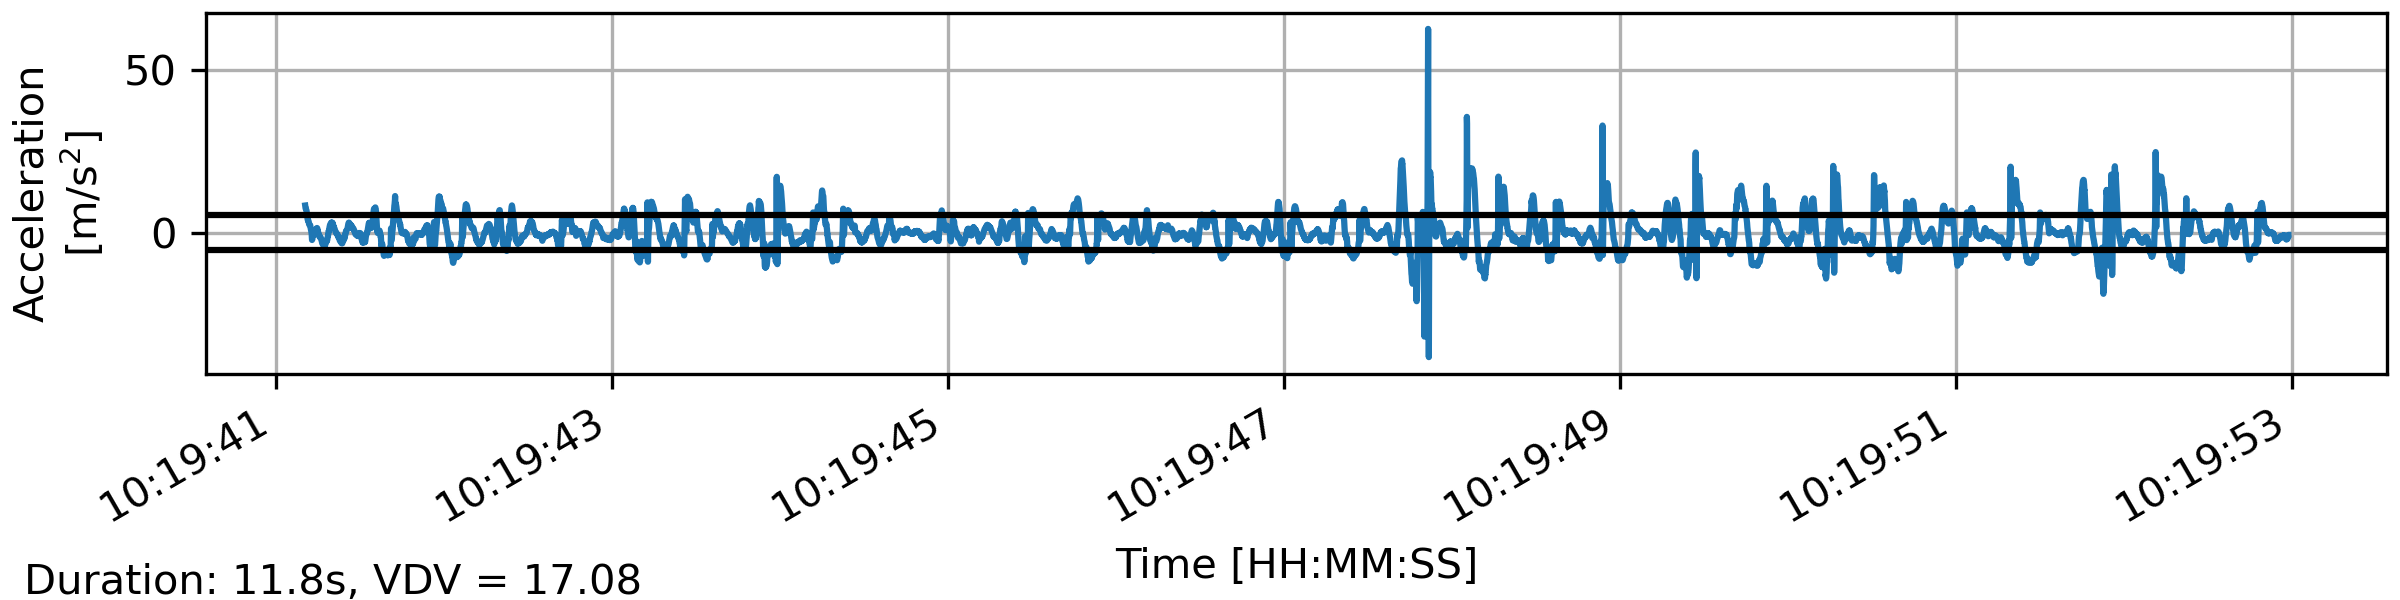
\includegraphics[width=160mm]{fig/session001-t2-aula-stroller-maxicosi-cot-0-SeatBotacc_ver-rep0.png}
  \caption{Raw seat pan vertical acceleration versus time from session 001:
  Maxi-Cosi Street Plus Stroller over the Sidewalk Slabs. Black horizontal lines
  indicate the \(\pm\)root mean square (RMS) about the mean and grey horizontal
  lines indicate the \(\pm\)vibration dose value (VDV) about the mean.}
  \label{fig:vert-acc-example}
\end{figure}

ISO~2631-1 provides weighting filters that highlight those frequencies adults
are most sensitive to. To apply them, we calculated the amplitude spectra of the
acceleration time histories of each trial using the Fast Fourier Transform
(FFT). Figure~\ref{fig:freq-spectrum} gives an example of a raw amplitude
spectrum along with smoothened versions of the raw and ISO 2631-1 weighted
signals. In almost all trials, there is a single dominant peak frequency in the
ISO weighted and smoothed spectra. For the few trials that had two or more peaks
at approximately the same amplitude, the second peak was sometimes selected.
After ISO weighting, the area under the spectrum curve was calculated and the
frequency below which 80\% of the amplitude content falls marked as an indicator
of bandwidth.
%
\begin{figure}
  \centering
  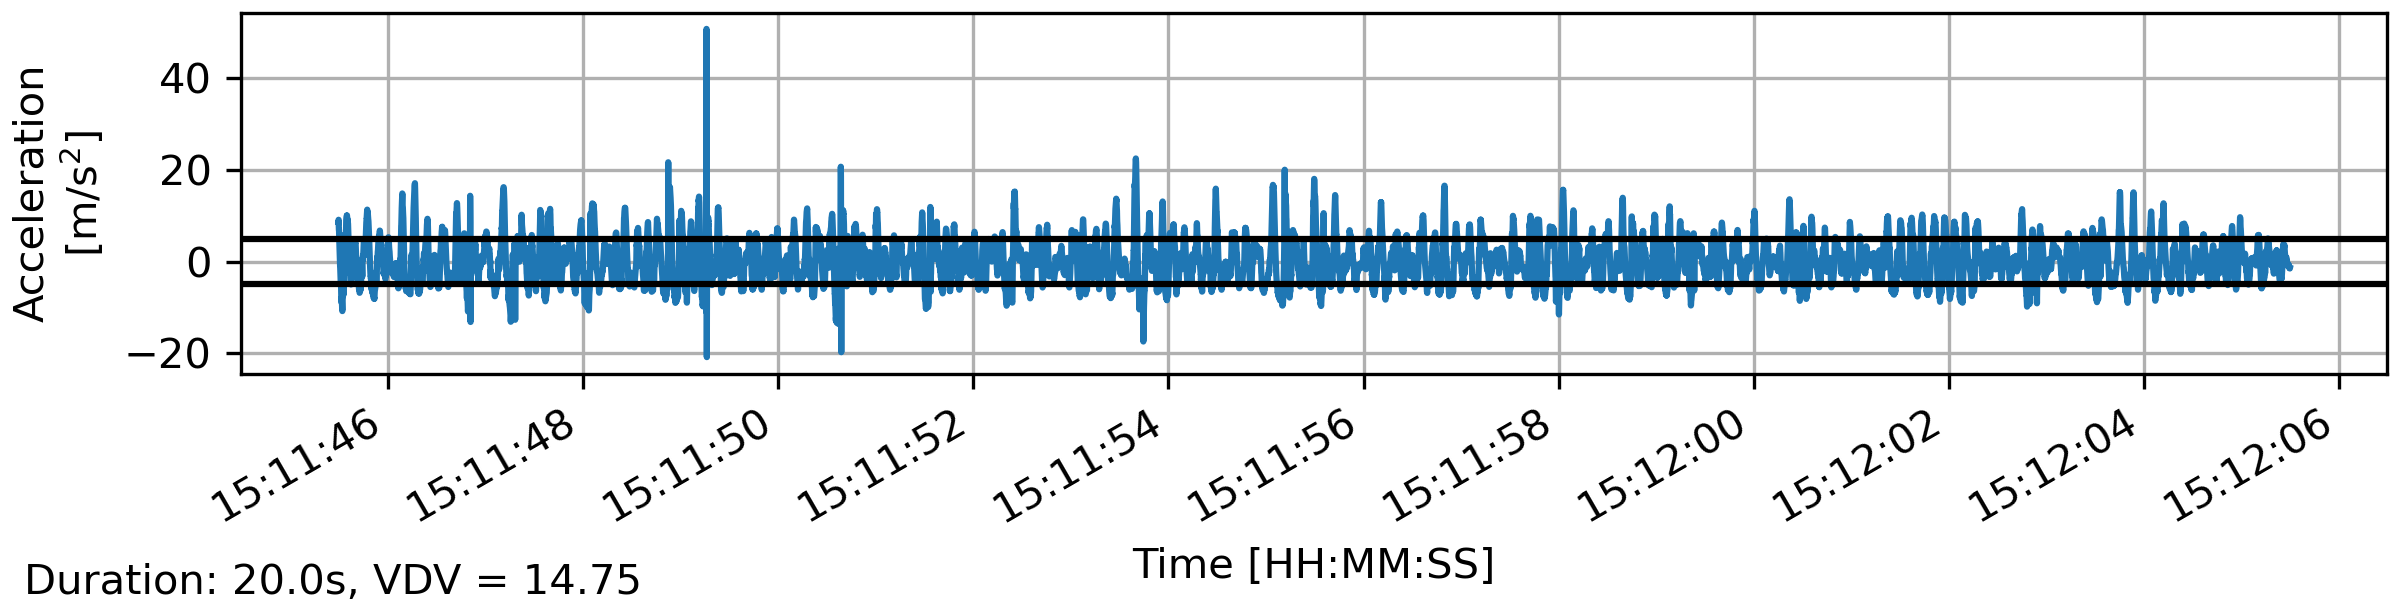
\includegraphics[width=160mm]{fig/session004-t0-pave-stroller-maxicosi-cot-0-SeatBotacc_ver-rep0.png}
  \caption{Seat pan vertical acceleration amplitude spectrum from session 004:
  Maxi-Cosi Street Plus over cobblestones. The gray curve shows the result of
  the FFT, the black line is a smoothed version of the FFT (zero-lag Butterworth
  low pass), and the blue line is the smoothed ISO weighted FFT. The blue dashed
  vertical line indicates the frequency at the maximum amplitude of the smoothed
  curve. The blue dashed-dotted vertical line indicates the bandwidth threshold
  for 80\% of the area under the blue curve.}
  \label{fig:freq-spectrum}
\end{figure}

We calculated the root mean square (RMS) over \(N\) samples of the downsampled,
low-pass filtered, and ISO 2631-1 weighted vertical component of acceleration
\(a_{w,z}\) at the seat pan for each trial using Equation~\ref{eq:rms-acc} to
use for the health assessment and the RMS of the magnitude of the acceleration
vector at the seat pan using Equation~\ref{eq:rms-acc-mag} for the comfort
assessment, as per ISO 2631-1 guidelines. We set the ISO~2631-1 adjustment
factors \(k_x,k_y,k_z\) equal to 1 for all acceleration components. RMS gives an
indication of the average vertical acceleration experienced at the infant's
buttocks-seat interface for the duration of the trial and can be seen in
Figure~\ref{fig:vert-acc-example}. It is the primary metric recommended by
ISO-2631-1 for evaluation of health and comfort in adult whole-body vibration.
We also calculated the vibration dose value (VDV) of the \(M\) raw data vertical
acceleration \(a_{z}\) samples with Equation~\ref{eq:vdv-acc}, seen in
Figure~\ref{fig:vert-acc-example}. Lastly, we compute the crest factor and
absolute maximum of the downsampled and low pass filtered vertical
acceleration\footnote{Some scenarios have crest factors larger than 9, but we
do not report metrics other than RMS as ISO~2631-1 recommends for this study.}
with Equations~\ref{eq:crest-factor} and \ref{eq:max-acc}, respectively. All of
these per-repetition metrics are reported as mean values over the repetitions
corresponding to a scenario in Table~\ref{tab:results} in
Appendix~\ref{app:results}. Regarding the shock test, the analysis was conducted
on unfiltered data (not downsampled). We selected the maximum (absolute) peak
from the time history of the vertical acceleration of the seat pan starting from
the events' time histories (Figure \ref{fig:shock_time-history}), limiting it to
16~g when the peak exceeded that maximum. The following equations give the
details of the metrics calculations:
%
\begin{align}
  \textrm{RMS}_{a_{w,z}} = \sqrt{\frac{1}{N}\sum_{n=1}^{N} k_z^2 a_{w,z}^2(t_n)}
  \label{eq:rms-acc}
\end{align}

\begin{align}
  \textrm{RMS}_{a_{w,xyz}} = \sqrt{\frac{1}{N}\sum_{n=1}^{N} k_x^2 a_{w,x}^2(t_n) + k_y^2 a_{w,y}^2(t_n) + k_z^2 a_{w,z}^2(t_n)}
  \label{eq:rms-acc-mag}
\end{align}

\begin{align}
  \textrm{VDV}_{a_{z}} = \left(\frac{1}{M}\sum_{m=1}^{M} a_{z}^4(t_m)\right)^{1/4}
  \label{eq:vdv-acc}
\end{align}

\begin{align}
  \textrm{Crest Factor}_{a_{z}} =\frac{\max|a_{z}(t_m)|}{\sqrt{\frac{1}{M}\sum_{m=1}^{M} a_{z}^2(t_m)}}
  \label{eq:crest-factor}
\end{align}

\begin{align}
  \textrm{MAX}_{a_{z}} =\max|a_{z}(t_n)|
  \label{eq:max-acc}
\end{align}

\begin{figure}
  \centering
  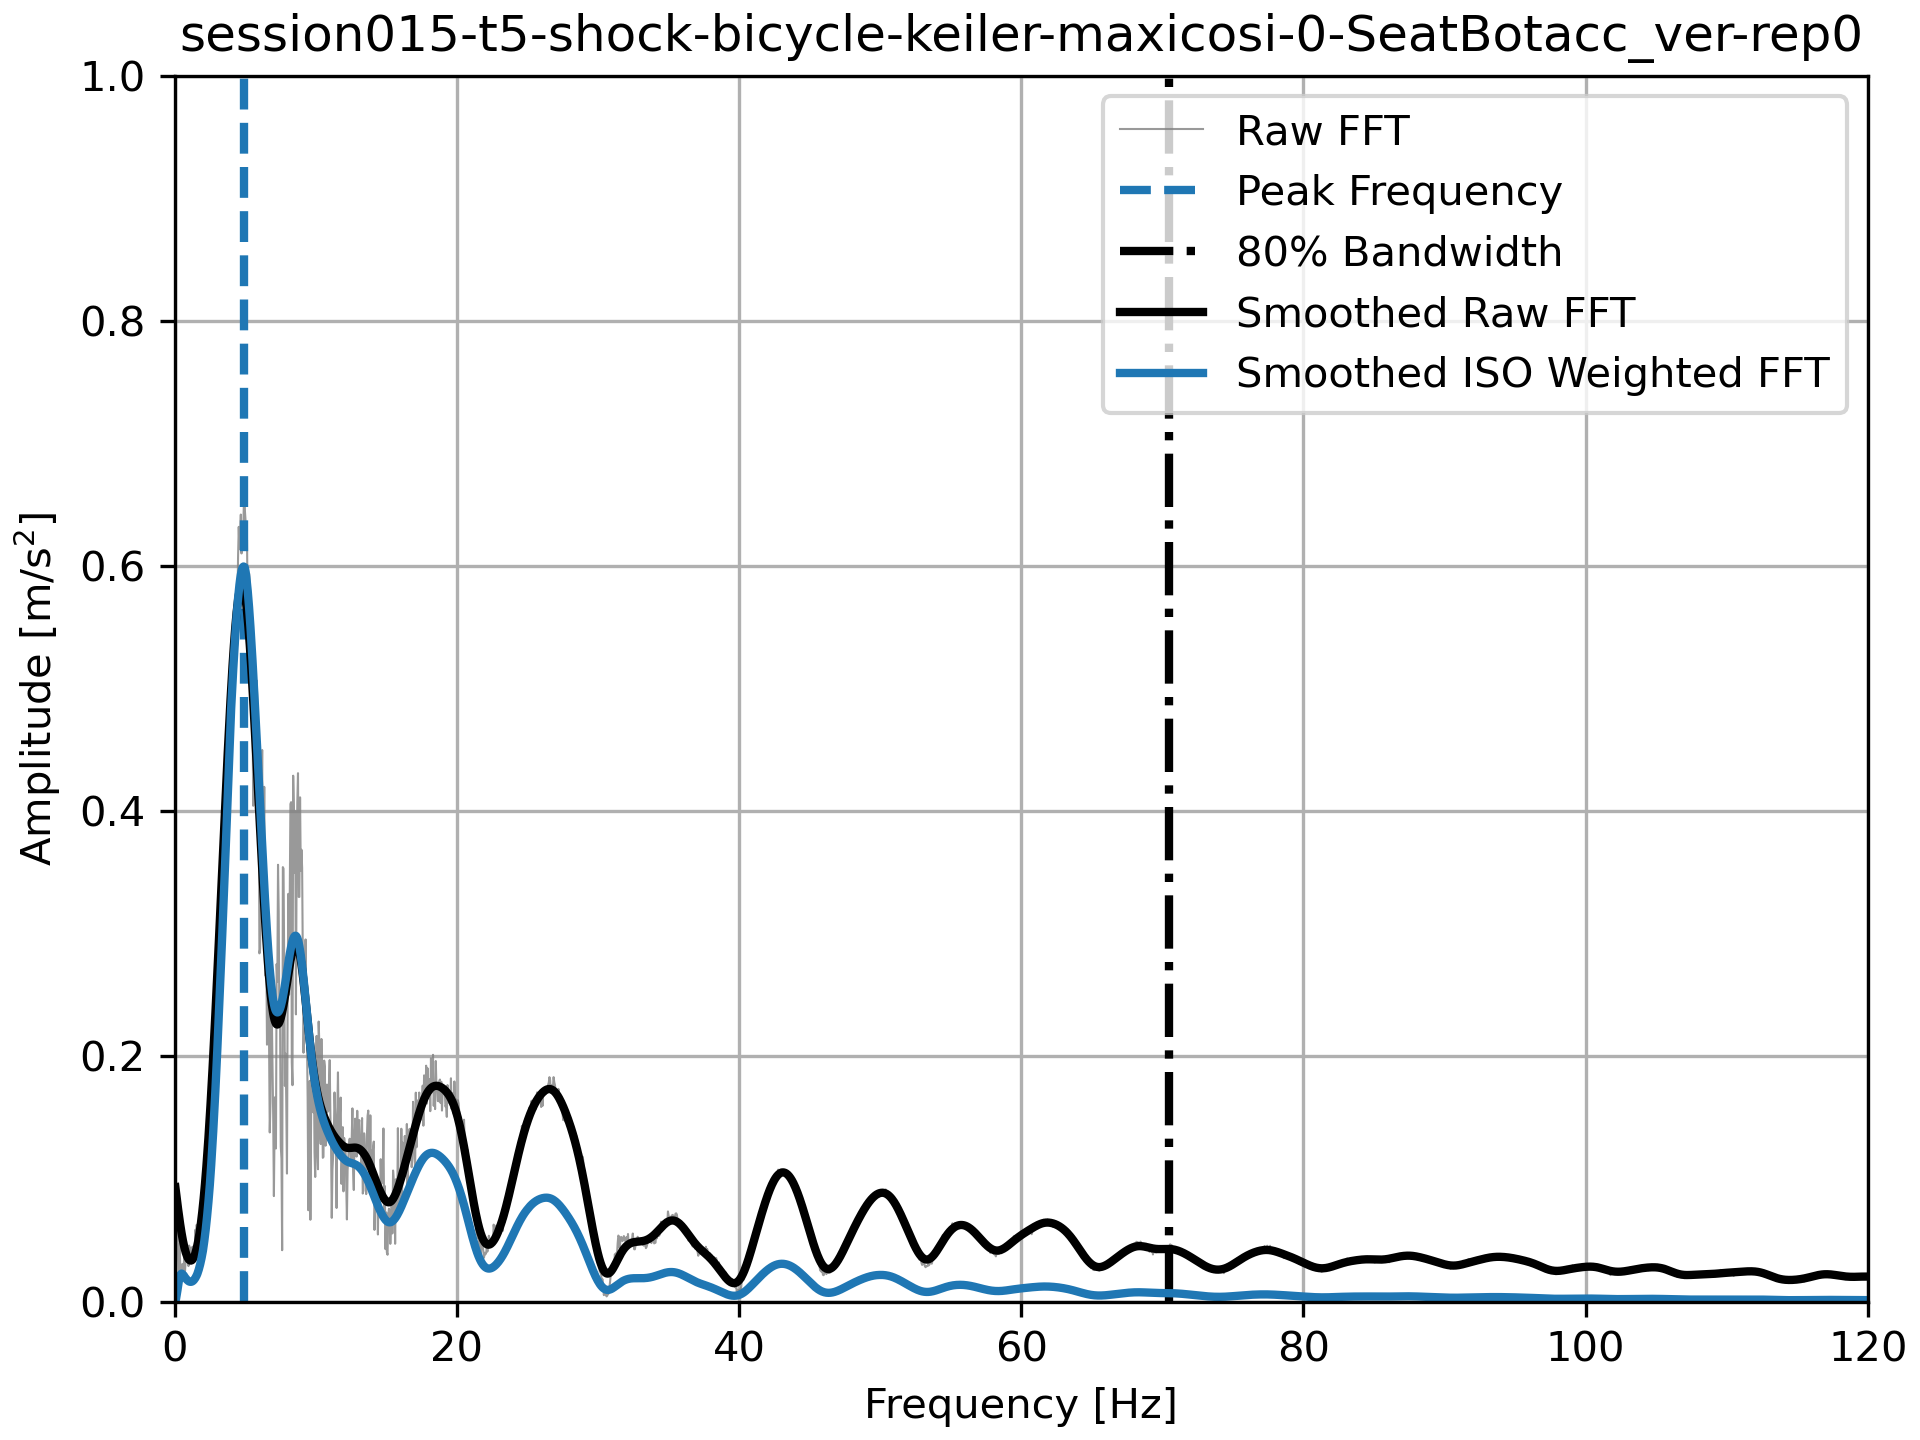
\includegraphics[width=160mm]{fig/session015-t5-shock-bicycle-keiler-maxicosi-0-SeatBotacc_ver-rep0.png}
  \caption{Raw seat pan vertical acceleration versus time from session 015:
  Keiler tricycle during the shock test.}
  \label{fig:shock_time-history}
\end{figure}

\subsection{Statistical Modelling}
%
To determine how road surface and stroller setup predict ISO~2631-1 weighted
vertical RMS acceleration, we fit an ordinary linear least squares model to the
data using:
%
\begin{align}
  \textrm{RMS}_{a_{w,z}} = 
  \beta_0 +
  \beta_1 x_\textrm{Road Surface} +
  \beta_2 x_\textrm{Stroller} +
  \epsilon
\end{align}
%
Both \(x_\textrm{Road Surface}\) and \(x_\textrm{Stroller}\) are categorical
variables and we select tarmac and the Green Machine as the reference values
when coding the categorical variables, respectively. We do not consider the
interaction of road surface and stroller.

To determine how speed, road surface, and cargo bicycle setup predict ISO~2631-1
weighted vertical RMS acceleration, we fit an ordinary linear least squares
model to the data using:
%
\begin{align}
  \textrm{RMS}_{a_{w,z}} = 
  \kappa_0 +
  \kappa_1 x_\textrm{Road Surface} +
  \kappa_2 x_\textrm{Cargo Bicycle} + 
  \kappa_3 x_\textrm{Speed} +
  \kappa_4 x_\textrm{Road Surface} \times x_\textrm{Speed} +
  \epsilon
\end{align}
%
Both \(x_\textrm{Road Surface}\) and \(x_\textrm{Cargo Bicycle}\) are
categorical variables and \(x_\textrm{Speed}\) is a continuous variable. We
select tarmac and the `Keiler, Maxi-Cosi seat, 0 mo' setup as the reference
values when coding the categorical variables, respectively. We do not consider
the interaction of road surface and cargo bicycle setup, but we do consider the
interaction of speed with road surface. We use \(p<0.05\) to indicate
significant differences for both models. Following fitting the two statistical
models, we apply Tukey's Range Test to compare vehicle setups among each other
for the different road surfaces and speed ranges with \(p=0.05\) for the
adjusted limit for significance.

\section{Results}
%
\subsection{Effect of Speed with Cargo Bicycles}
%
Figure~\ref{fig:compare-bicycle-speed} shows the variation in ISO~2631-1
weighted vertical RMS acceleration across the tested speeds. Accelerations
experienced when riding over the paver bricks were always larger than for tarmac
at the same speed, with the paver bricks showing about a 4-5\(\times\) higher
acceleration magnitude than tarmac. Over paver bricks, the RMS acceleration
increased by about 1.6\(\times\) when increasing the speed from
\SIrange{12}{25}{\kilo\meter\per\hour}. The effect of speed while cycling over
tarmac was less drastic but also may show a slight increase of accelerations
over the speed range.
%
\begin{figure}
  \centering
  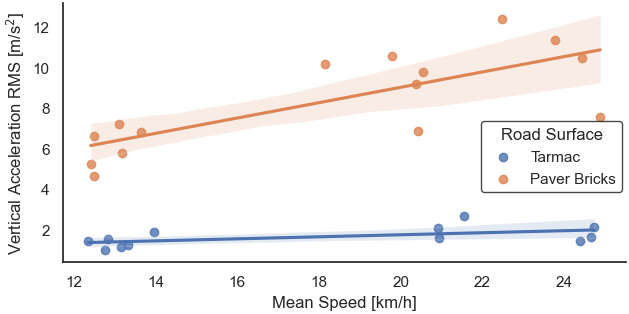
\includegraphics[width=160mm]{fig/SeatBotacc_ver-bicycle-speed-compare.png}
  \caption{Seat pan ISO 2631-1 weighted vertical acceleration RMS versus speed
  for all cargo bicycle repetitions. Shaded regions represent the 95\%
  confidence intervals from a simple linear regression that ignores
  \(x_\textrm{Cargo Bicycle}\).}
  \label{fig:compare-bicycle-speed}
\end{figure}

\subsection{Effect of Dummy Size}
%
Figure~\ref{fig:compare-baby-mass} shows the ISO~2631-1 weighted vertical RMS
acceleration for each repetition for all vehicles, comparing among dummy sizes.
There were larger accelerations in the bicycle (high speeds) versus the stroller
(low speeds), likely mostly attributed to the different testing speeds. When
comparing the vertical RMS acceleration values between cargo bicycles and
strollers there are no obvious differences due to baby size, i.e. each dummy
size experienced a similar range of acceleration magnitudes when vehicle type
and road surface are ignored. For the bicycles, the lightest dummy sometimes
experienced higher acceleration than the heavier dummy, but high and low
accelerations are seen across the speed range tested.
%
\begin{figure}
  \centering
  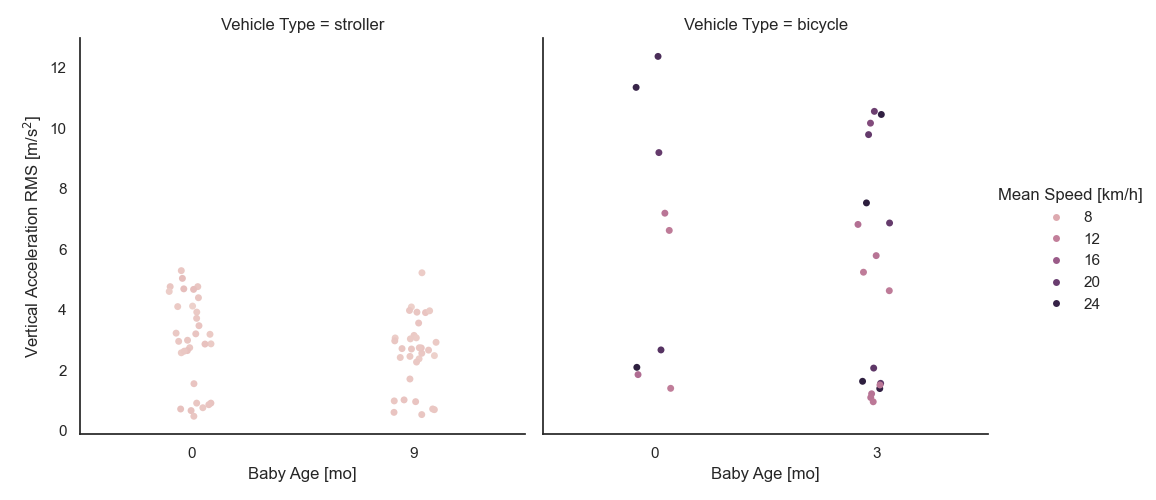
\includegraphics[width=160mm]{fig/SeatBotacc_ver-baby-mass-compare.png}
  \caption{Seat pan ISO~2631-1 weighted vertical RMS acceleration grouped by
  baby age (and thus size \& mass) for all repetitions with colour indicating
  the mean speed of the trial. The lightest colour dots are strollers and the
  remaining are cargo bicycles.}
  \label{fig:compare-baby-mass}
\end{figure}

\subsection{Effect of Road Surface}
%
Figure~\ref{fig:compare-road-surface} shows ISO~2631-1 weighted vertical RMS
acceleration from repetitions grouped into the various road surfaces tested. All
vehicles were tested on paver bricks and tarmac but only strollers were tested
on cobblestones and sidewalk pavers and sidewalk slabs, i.e. light colour dots
(strollers are present in each column).
It is notable that tarmac almost always induced lower RMS acceleration than
other road types regardless of speed and vehicle type.
The sidewalk slabs and cobblestones have very similar acceleration ranges for
all strollers.
Paver bricks and sidewalk pavers seem to have a similar range of RMS
acceleration for the same 5~\si{\kilo\meter\per\hour} walking speeds.
Paver bricks cause relatively large accelerations at high travel speeds in the
cargo bicycles.
%
\begin{figure}
  \centering
  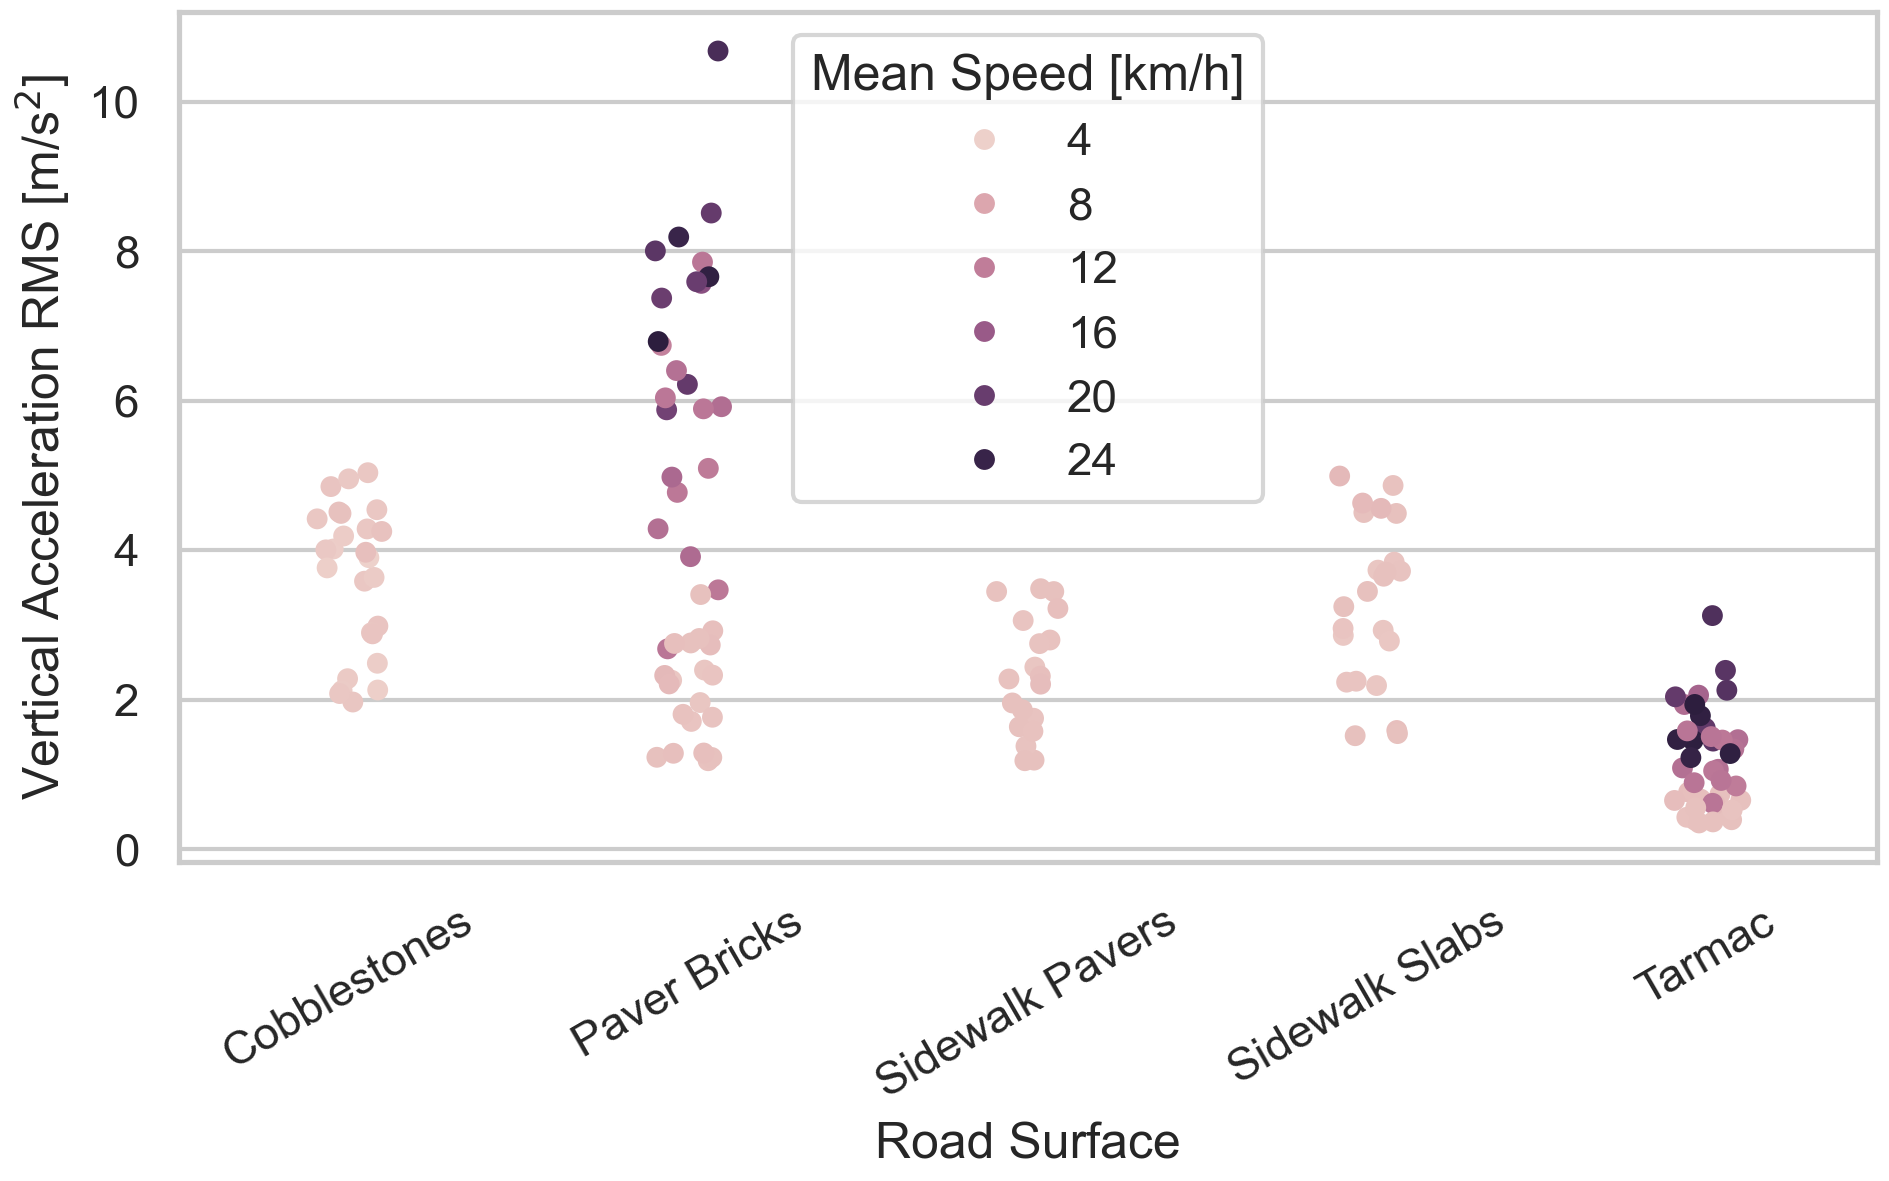
\includegraphics[width=160mm]{fig/SeatBotacc_ver-road-surface-compare.png}
  \caption{Seat pan ISO 2631-1 weighted vertical RMS acceleration grouped by
  road surface with colour indicating the mean speed of the repetition. The
  lightest colour dots are strollers and the rest are cargo bicycles.}
  \label{fig:compare-road-surface}
\end{figure}

\subsection{Effect of Vehicle Model}
%
Figure~\ref{fig:stroller-type-compare} shows the vertical RMS accelerations for
each road surface for each of the five strollers, lumping seat configurations
and dummy sizes. The Maxi-Cosi Street Plus and Stokke BABYZEN YOYO 0+ strollers
have similar mean values across repetitions. The Bugaboo Fox 5 has a slightly
lower mean for cobblestones, paver bricks, and sidewalk pavers. The Green
Machine performs better than the modern strollers on paver bricks, but similarly
otherwise. The Old Rusty performs better than the modern strollers on all
surfaces except tarmac. All strollers seem to experience the same acceleration
on tarmac. There may be no significant difference in the acceleration
experienced in each modern stroller model. All road surfaces compared to tarmac
cause at least double the RMS acceleration.
%
\begin{figure}
  \centering
  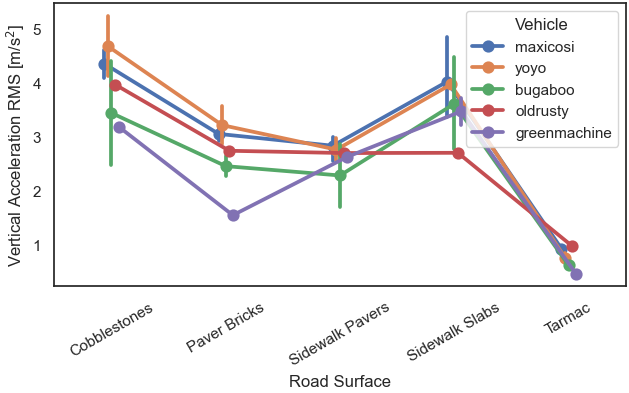
\includegraphics[width=160mm]{fig/SeatBotacc_ver-stroller-type-compare.png}
  \caption{Mean seat pan ISO 2631-1 weighted vertical RMS acceleration per road
  surface for each stroller. Vertical lines indicate the standard deviation for
  categories that have more than one repetition.} 
  \label{fig:stroller-type-compare}
\end{figure}

Figure~\ref{fig:bicycle-type-compare} compares the two cargo bicycle models we
tested. Each cargo bicycle was fitted with the same set of two baby seats (Melia
baby shell and Maxi-Cosi Pebble Pro baby seat). On tarmac the two-wheel cargo
bicycle delivers lower accelerations to the seat pan, but on paver bricks the
two vehicles show little difference in RMS accelerations. Both vehicles show
increasing vertical RMS acceleration with speed.
%
\begin{figure}
  \centering
  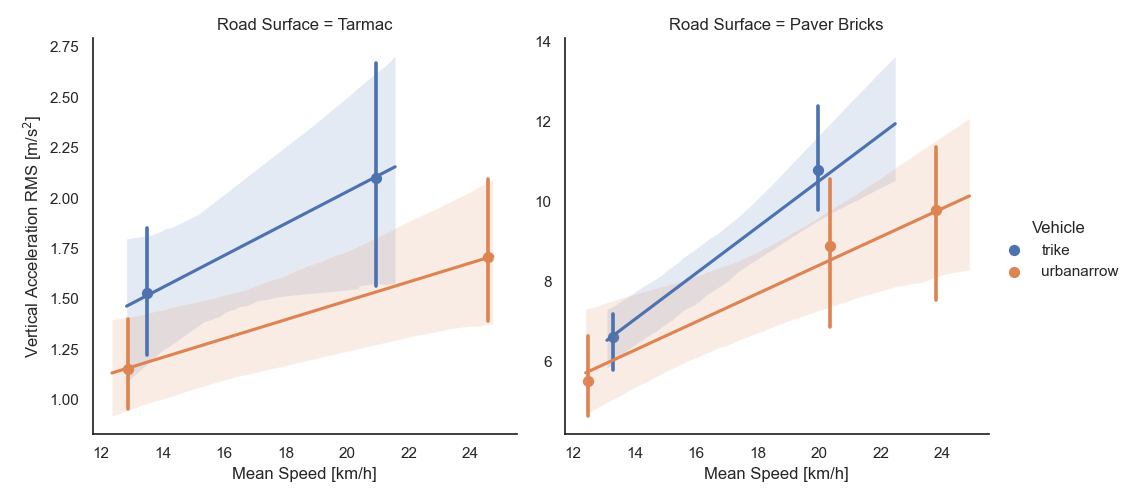
\includegraphics[width=160mm]{fig/SeatBotacc_ver-bicycle-type-compare.png}
  \caption{Seat pan ISO 2631-1 weighted vertical RMS acceleration versus speed
  grouped by road surface and cargo bicycle model. Slanted lines indicate a
  linear regression, vertical lines are the standard deviation at those speeds,
  and shaded regions show the 95\% confidence intervals for the regression.}
  \label{fig:bicycle-type-compare}
\end{figure}

\subsection{Dominant Frequency and Bandwidth}
%
Figure~\ref{fig:peak-freq-dist} shows the distributions of dominant (peak)
frequency compared among road surface types for each of the target speeds. Peak
frequencies range from about \SIrange{4}{11}{\hertz} across all trials. For
strollers (5~\si{\kilo\meter\per\hour}), the median frequency increases from
sidewalk slabs to cobblestones and sidewalk pavers and then to tarmac and paver
bricks. The peak frequency median does not correlate sequentially with the
geometric width of the dimension of the road surface feature. For the cargo
bicycles, difference in peak frequency between the two road surfaces is not so
apparent or consistent.
%
\begin{figure}
  \centering
  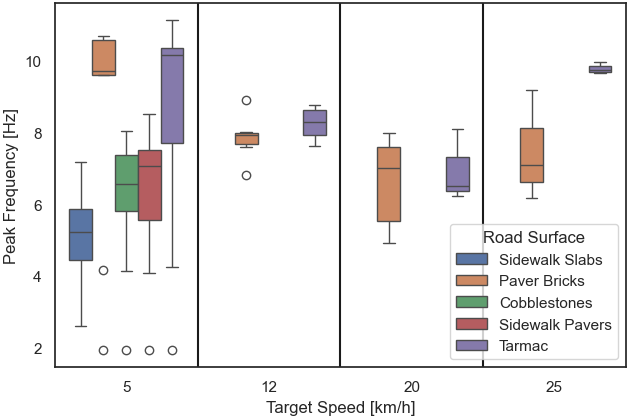
\includegraphics[width=160mm]{fig/SeatBotacc_ver-peak-freq-dist.png}
  \caption{Peak frequency distributions comparisons among road surfaces for each
  target speed group for non-shock repetitions. The boxes bound the quartiles
  and indicate the median. The whiskers indicate the 95\textsuperscript{th}
  percentile and circles are any outliers.}
  \label{fig:peak-freq-dist}
\end{figure}

Figure~\ref{fig:bandwidth-dist} gives a general indication of bandwidth (80\% of
the amplitude spectrum content) distributions for each of the target speed
groups. Most frequency content is below 45~\si{\hertz} for all trials. The
median bandwidth across all trials is 20~\si{\hertz}. For the cargo bicycles,
the frequency content is spread wider for paver bricks than for tarmac, but for
strollers there is likely no significant difference in these surfaces. For
strollers, sidewalk pavers, sidewalk slabs, and cobblestones have similar
bandwidths. However this is based on the ISO filtering which attenuated the
higher frequencies. For the tested lying postures this weighting may have to be
reconsidered, as will be addressed further in the discussion. 
%
\begin{figure}
  \centering
  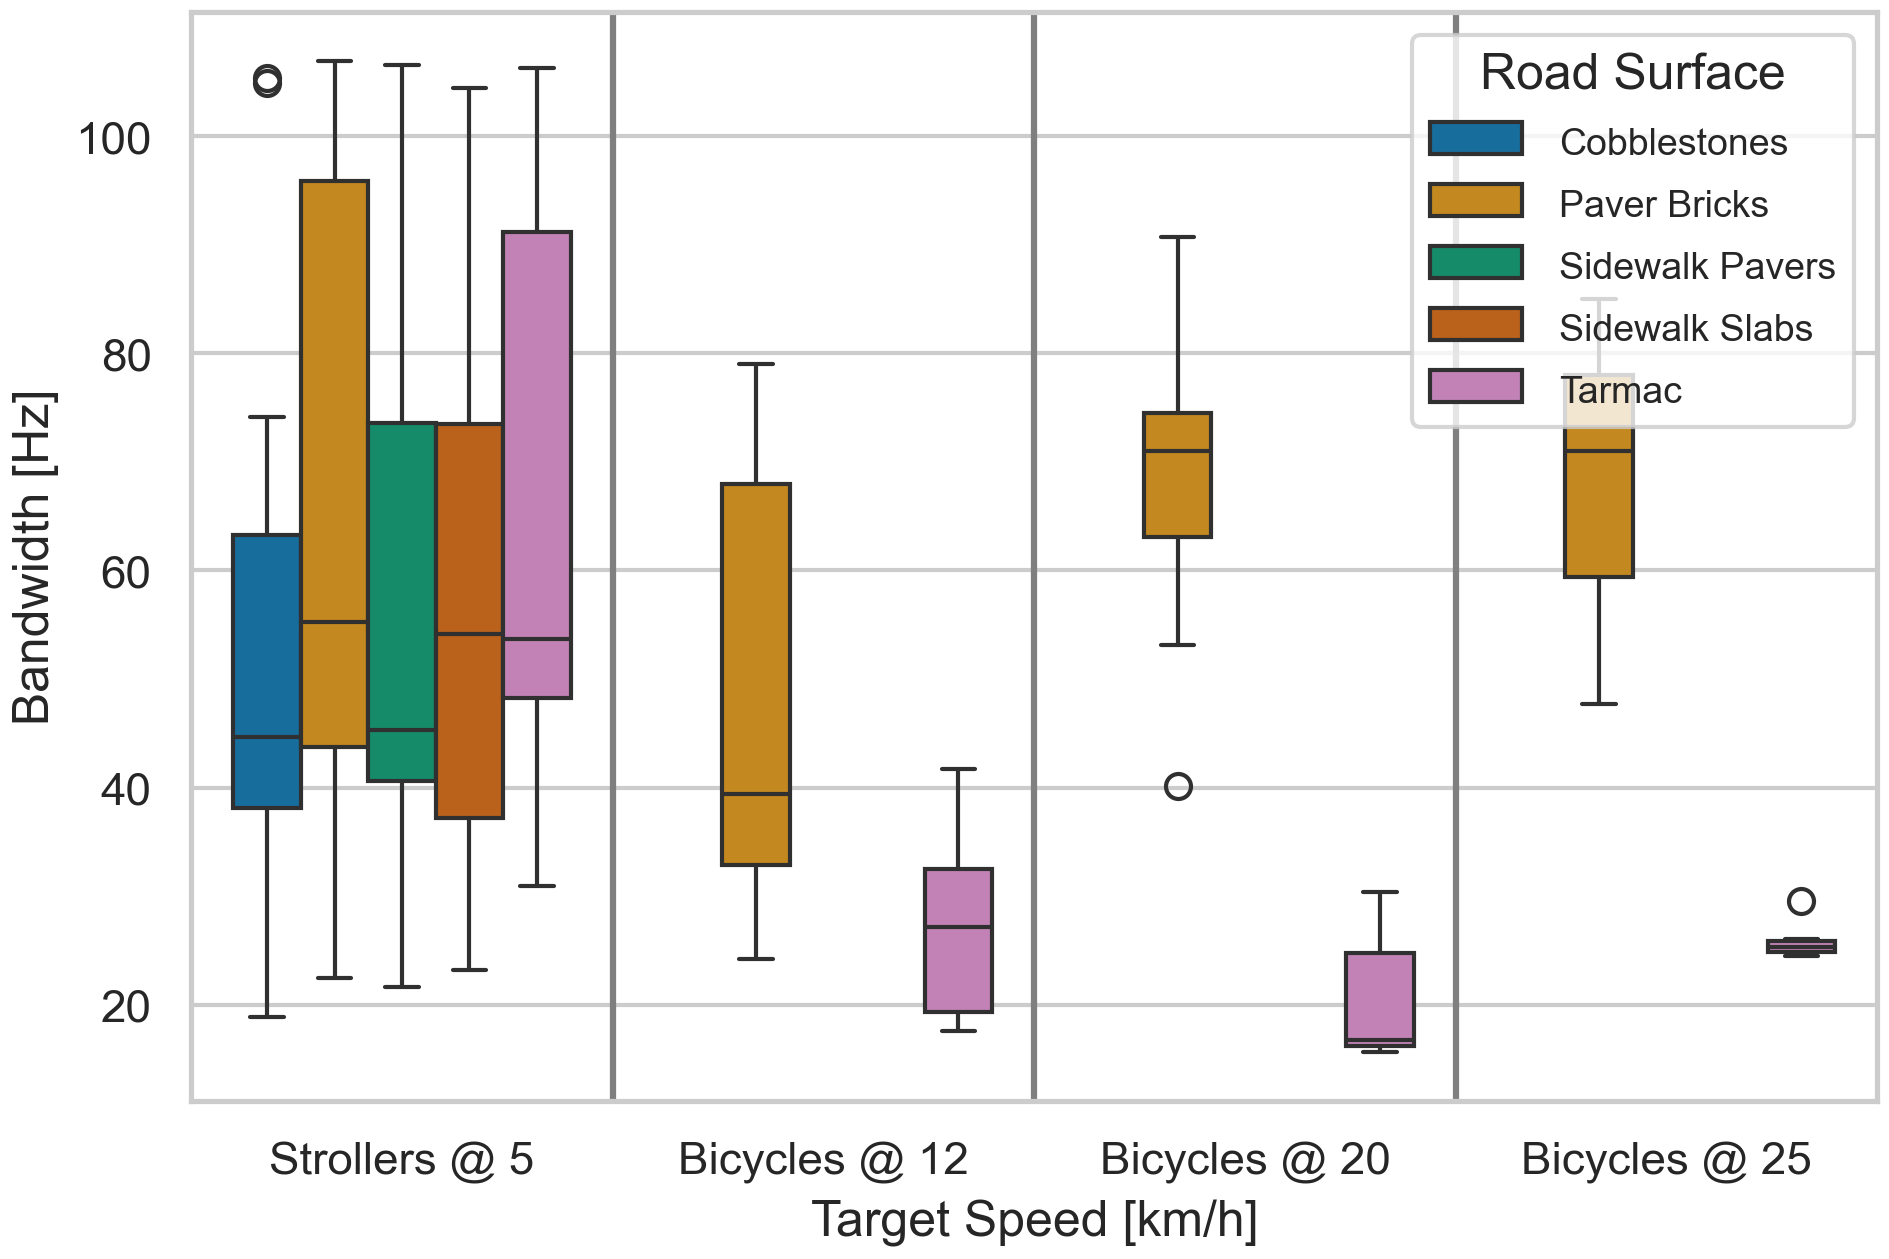
\includegraphics[width=160mm]{fig/SeatBotacc_ver-bandwidth-dist.png}
  \caption{Bandwidth (based on 80\% of the area under the ISO~2631-1 filtered
  amplitude spectrum) for each target speed group for non-shock repetitions. The
  boxes bound the quartiles and indicate the median. The whiskers indicate the
  95\textsuperscript{th} percentile and circles are any outliers.}
  \label{fig:bandwidth-dist}
\end{figure}

\subsection{Health Assessment}
\label{sec:health-assesment}
%
Figures \ref{fig:health-stroller} and \ref{fig:health-bicycle} show the
ISO~2631-1 weighted vertical acceleration at the seat pan for all repetitions of
the stroller and cargo bicycles, respectively. The horizontal lines in the
figure correspond to the boundary of the ``health caution'' and  ``health risk''
zones in the standard, which has a dependence on exposure duration. If
acceleration values are above the health caution zone, ISO~2631-1 states that
``health risks are likely'' for adults in erect seating postures for a
continuous daily dose. It must be emphasised that the ISO~2631-1 is based on
adults and may not result in a representative risk for infants or older
children.

\begin{figure}
  \centering
  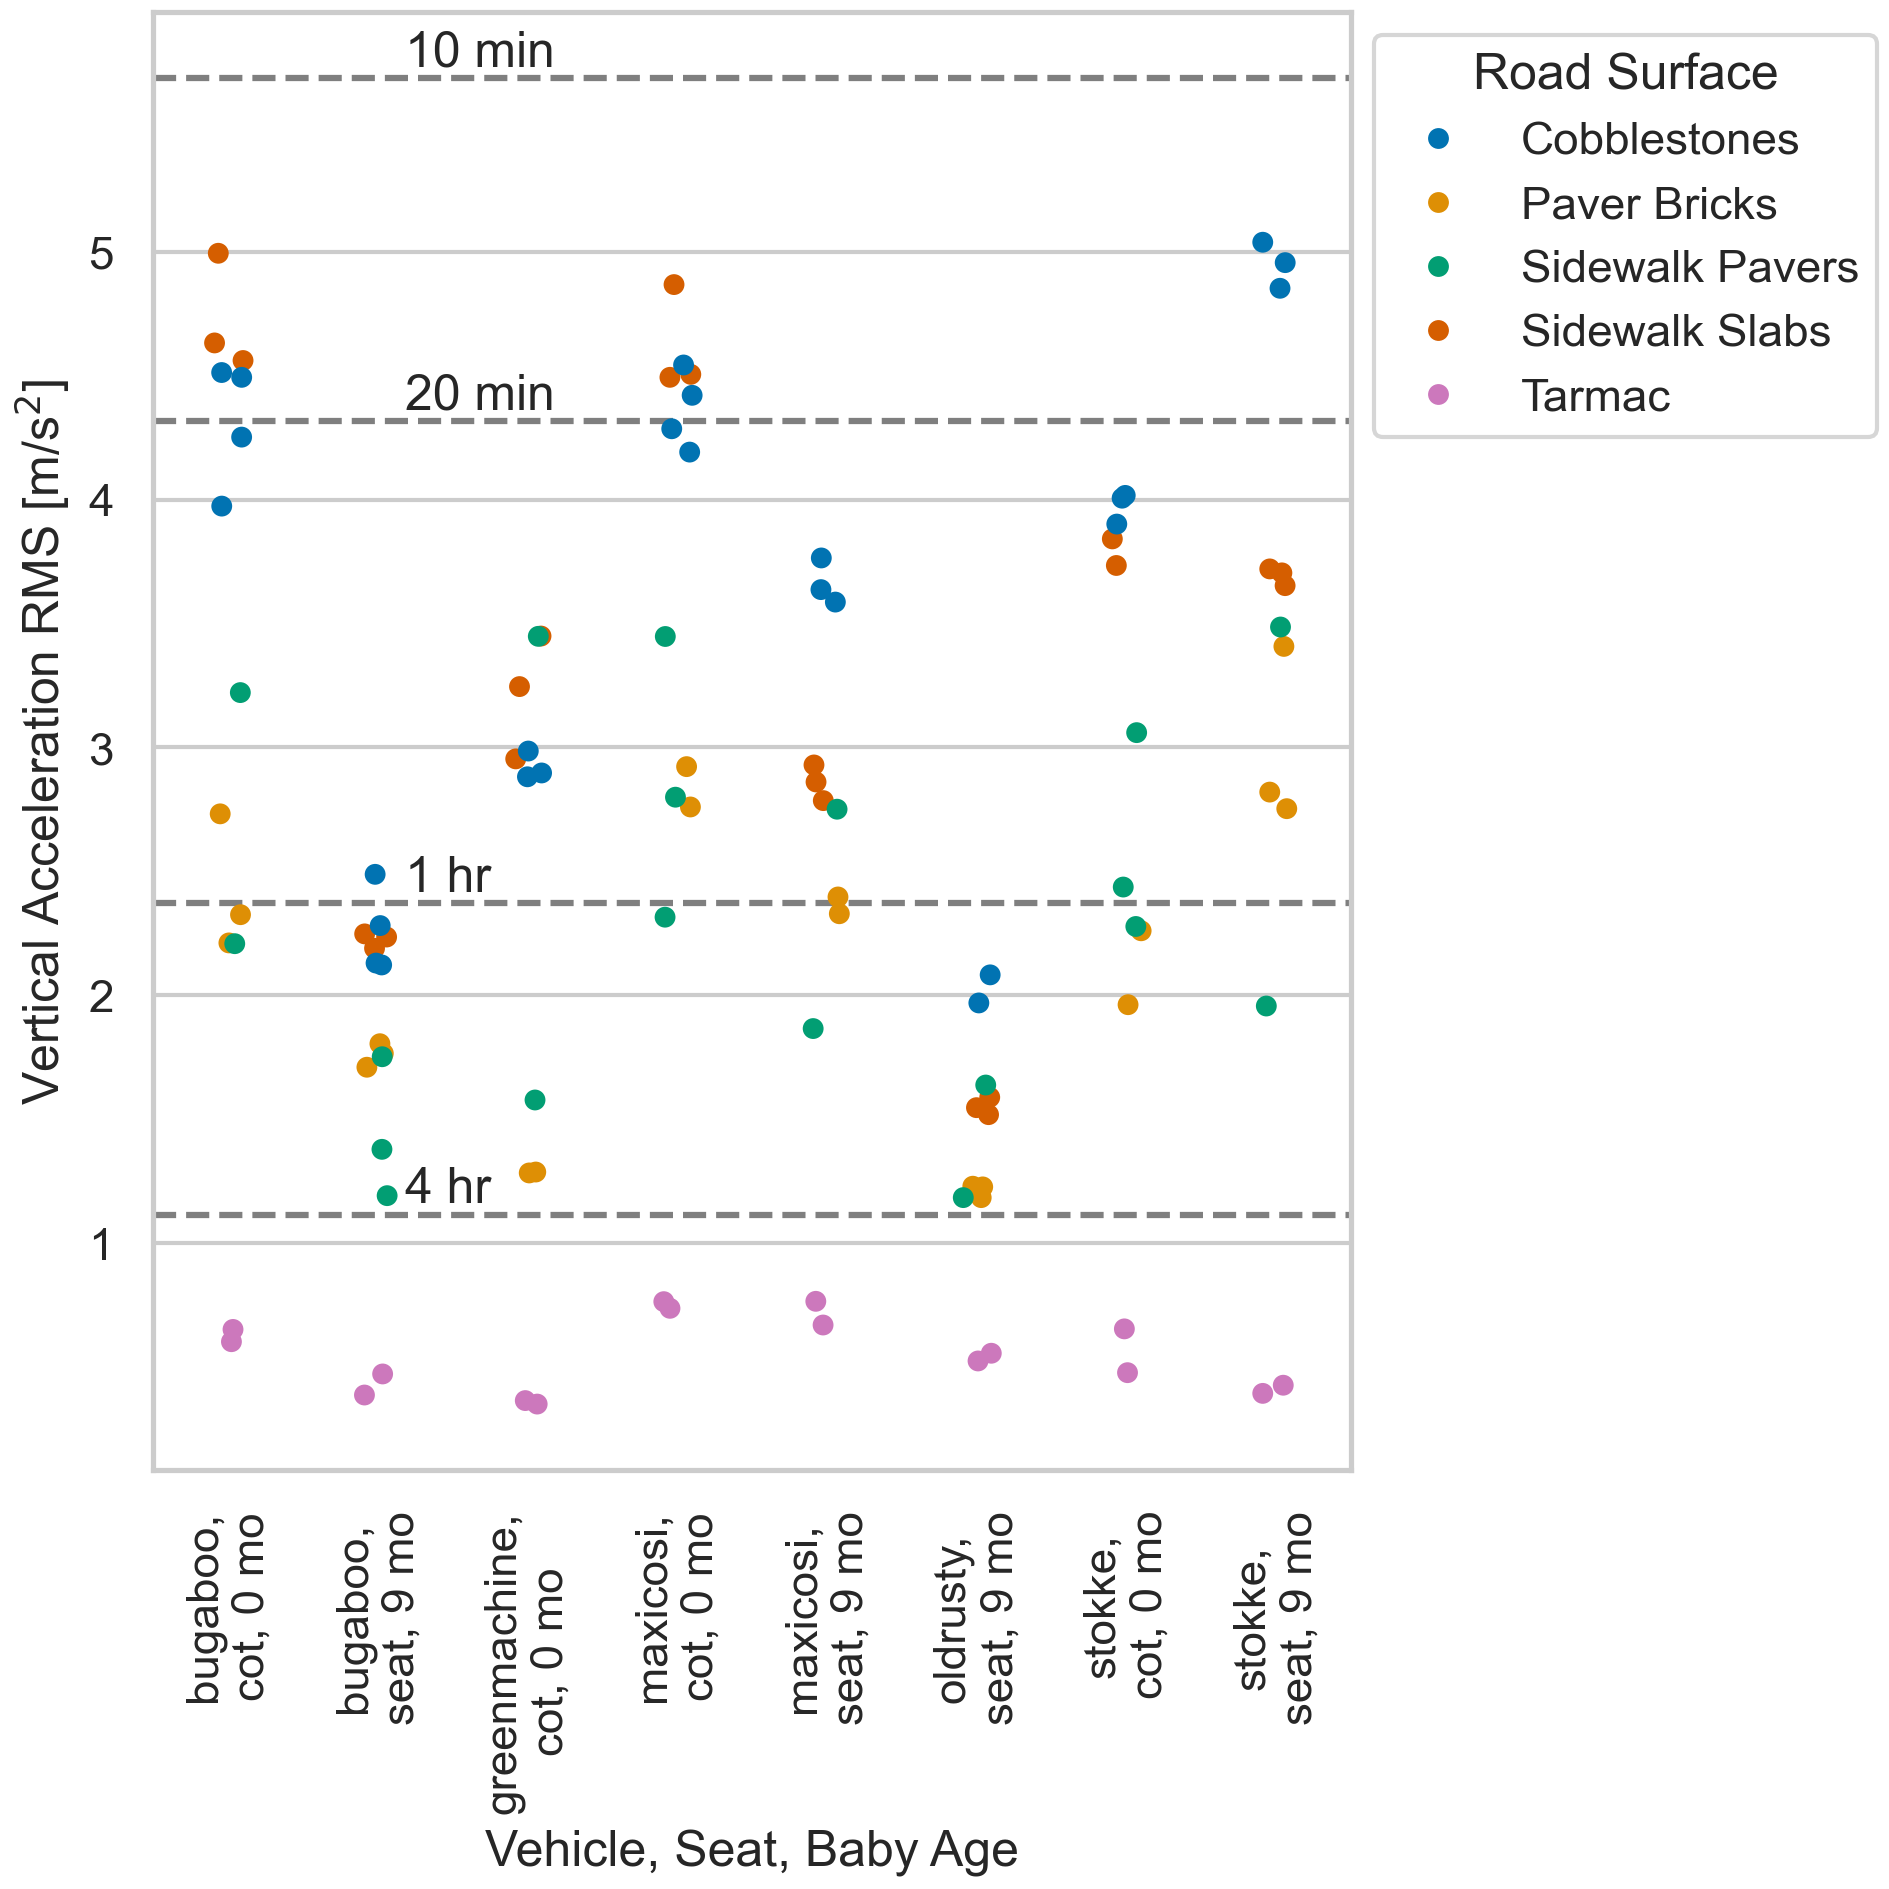
\includegraphics[width=160mm]{fig/SeatBotacc_ver-rms-stroller-compare-all.png}
  \caption{ISO~2631-1 weighted seat pan vertical RMS acceleration of all
  stroller repetitions with colour representing road surface. The horizontal
  dashed grey lines with time duration indicators are the upper bound of the
  ISO~2631-1 ``health caution zone'' at for adults seated erectly experiencing
  vibrations for continuous duration in a daily dose.}
  \label{fig:health-stroller}
\end{figure}
%
\begin{figure}
  \centering
  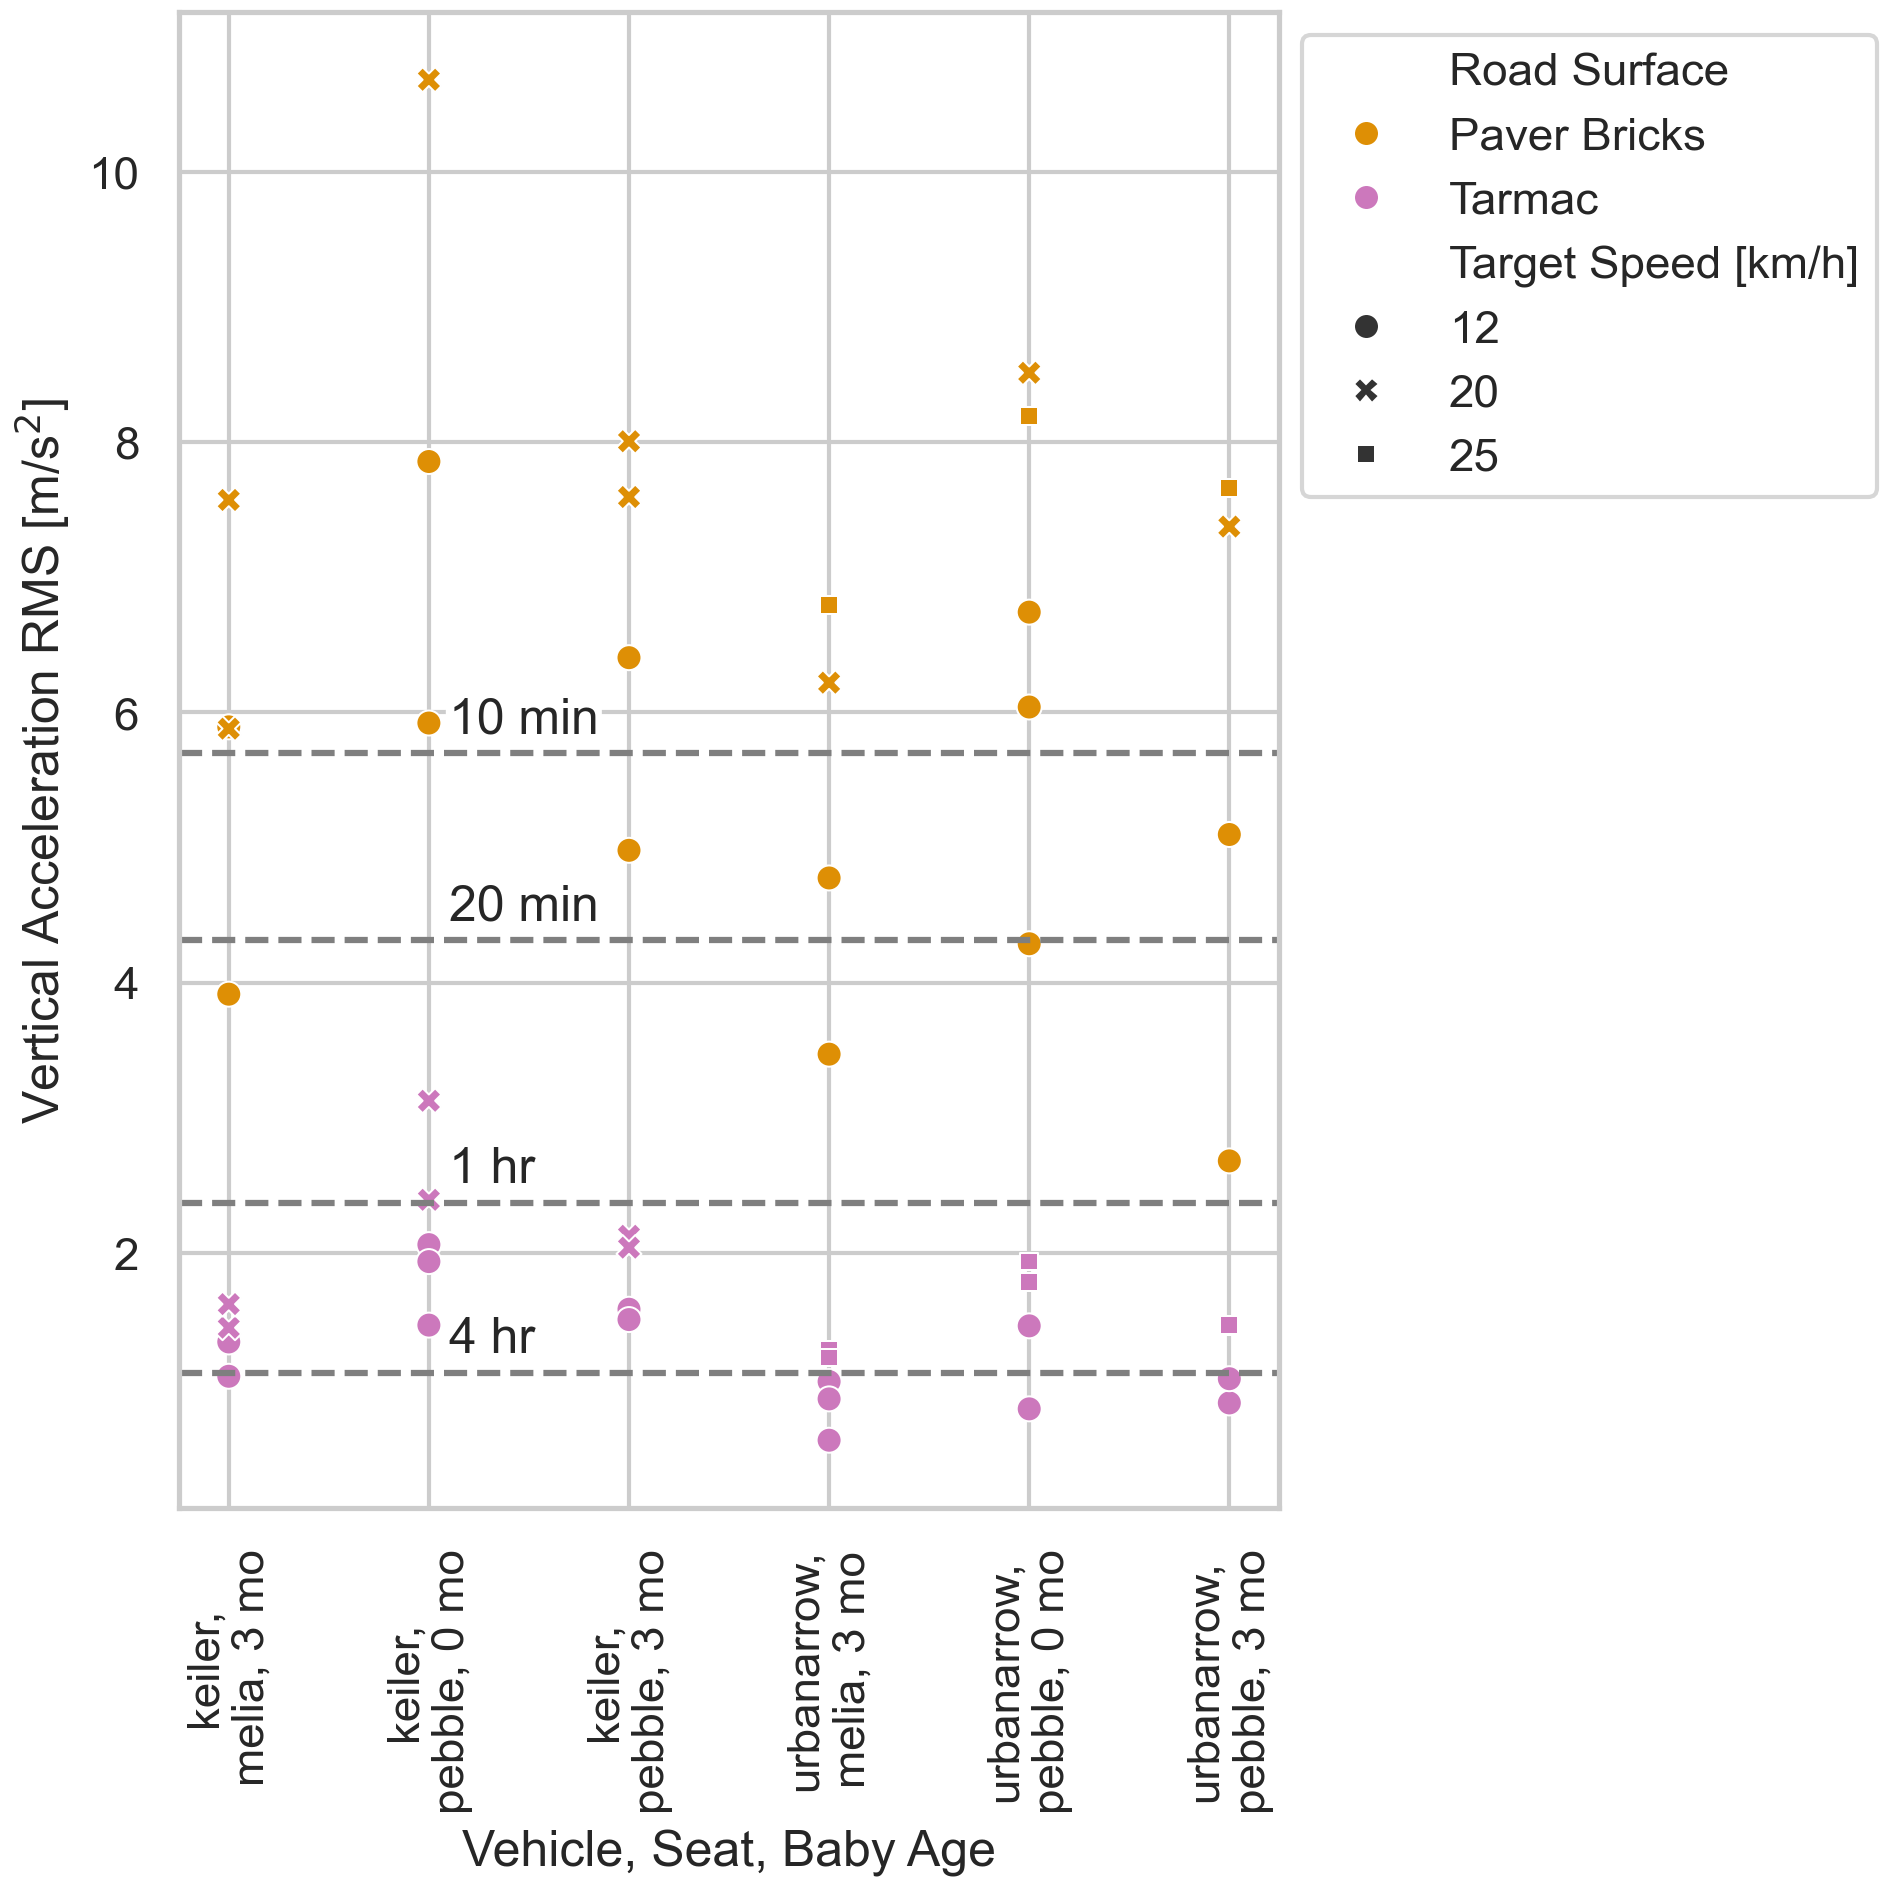
\includegraphics[width=160mm]{fig/SeatBotacc_ver-rms-bicycle-compare-all.png}
  \caption{ISO~2631-1 weighted seat pan vertical RMS acceleration of all cargo
  bicycle trials with colour representing road surface and marker style
  indicating the target speed. The horizontal dashed grey lines with time
  duration indicators are the upper bound of the ISO~2631-1 ``health caution
  zone'' for adults seated erectly experiencing vibrations for continuous
  duration in a daily dose.}
  \label{fig:health-bicycle}
\end{figure}

For the strollers, all vibration measurements were below the health caution zone
boundary if the daily continuous exposure is less than 10~\si{\minute}.
Additionally, all strollers pushed over tarmac were below the zone if the daily
continuous exposure is less than 4~\si{\hour}. Pushing the Bugaboo Fox 5 and
Maxi-Cosi Street Plus with a 0 month infant or the Stokke BABYZEN YOYO 0+ with a
9 month infant over cobblestones and sidewalk slabs may have health risks if the
duration exceeds 20~\si{\minute}. For almost all of the strollers pushing over
any surface except tarmac exceeded the 1~\si{\hour} risk boundary. Notably the
Bugaboo Fox 5 and Old Rusty with a 9 mo infant fell under the 1~\si{\hour}
threshold for all surfaces. The 0 month dummy experienced worse accelerations
than the 9 month dummy in the Bugaboo Fox 5 and Maxi-Cosi Street Plus, but that
was opposite for the Stokke YOYO 0+. Old rusty showed the least overall
acceleration magnitudes.

For both cargo bicycles, the accelerations exceeded the 10~\si{\minute} health
risk threshold when ridden above 20~\si{\kilo\meter\per\hour} on paver bricks
and exceeded the 1~\si{\hour} health risk threshold when ridden more than
1~\si{\hour} above 12~\si{\kilo\meter\per\hour} on paver bricks. All but the
Keiler with the Maxi-Cosi seat and the 0 mo dummy were under the 1~\si{\hour}
threshold for riding on tarmac at any target speed. Only the Urban Arrow with
the 3 month dummy is (mostly) under the 4~\si{\hour} threshold when ridden at
either speed over tarmac. The accelerations may be less when using the Meila
Baby Shell seat versus the Maxi-Cosi car seat, this is statistically considered
later in the results.

\subsection{Comfort Assessment}
%
ISO~2631-1 recommends using the magnitude of the weighted seat pan acceleration
vector for comfort assessment. Figures \ref{fig:comfort-stroller} and
\ref{fig:comfort-bicycle} plot RMS of the acceleration magnitude along with the
comfort indicators provided in the standard that are based on adults seated in
public transit for an unspecified duration. It must be emphasised that the
ISO~2631-1 comfort assessment is designed for adults and may not result in a
representative comfort assessment for infants or older children. We also include
a line representing cyclists' discomfort threshold reported by
Gao~et.~al~\cite{Gao2018}. It is important to recognize that cyclists perched on
a bicycle seat seem to tolerate more vibration discomfort than the public
transit riders who were surveyed for the ISO ratings. This points to possible
weakness in the ISO recommendations or to other factors affecting cycling
discomfort (e.g. the ability to stand on the pedals to lower vibration to the
body and the head).

When following the threshold definitions from the ISO~2631-1 guidelines for the
strollers, all are at least ``a little uncomfortable'' on all surfaces. All
strollers are ``fairly uncomfortable'' on tarmac. All other road surfaces are at
least ``very uncomfortable''. The `Bugaboo, seat, 9 mo' and `Green Machine, cot,
0 mo' over paver bricks and `Old Rusty, seat, 9 mo' over paver bricks, sidewalk
pavers, and sidewalk slabs are ``very uncomfortable'', but all other strollers
and surfaces are ``extremely uncomfortable''. The Old Rusty is the only stroller
that falls under the cyclist threshold discomfort line for all surfaces.
%
\begin{figure}
  \centering
  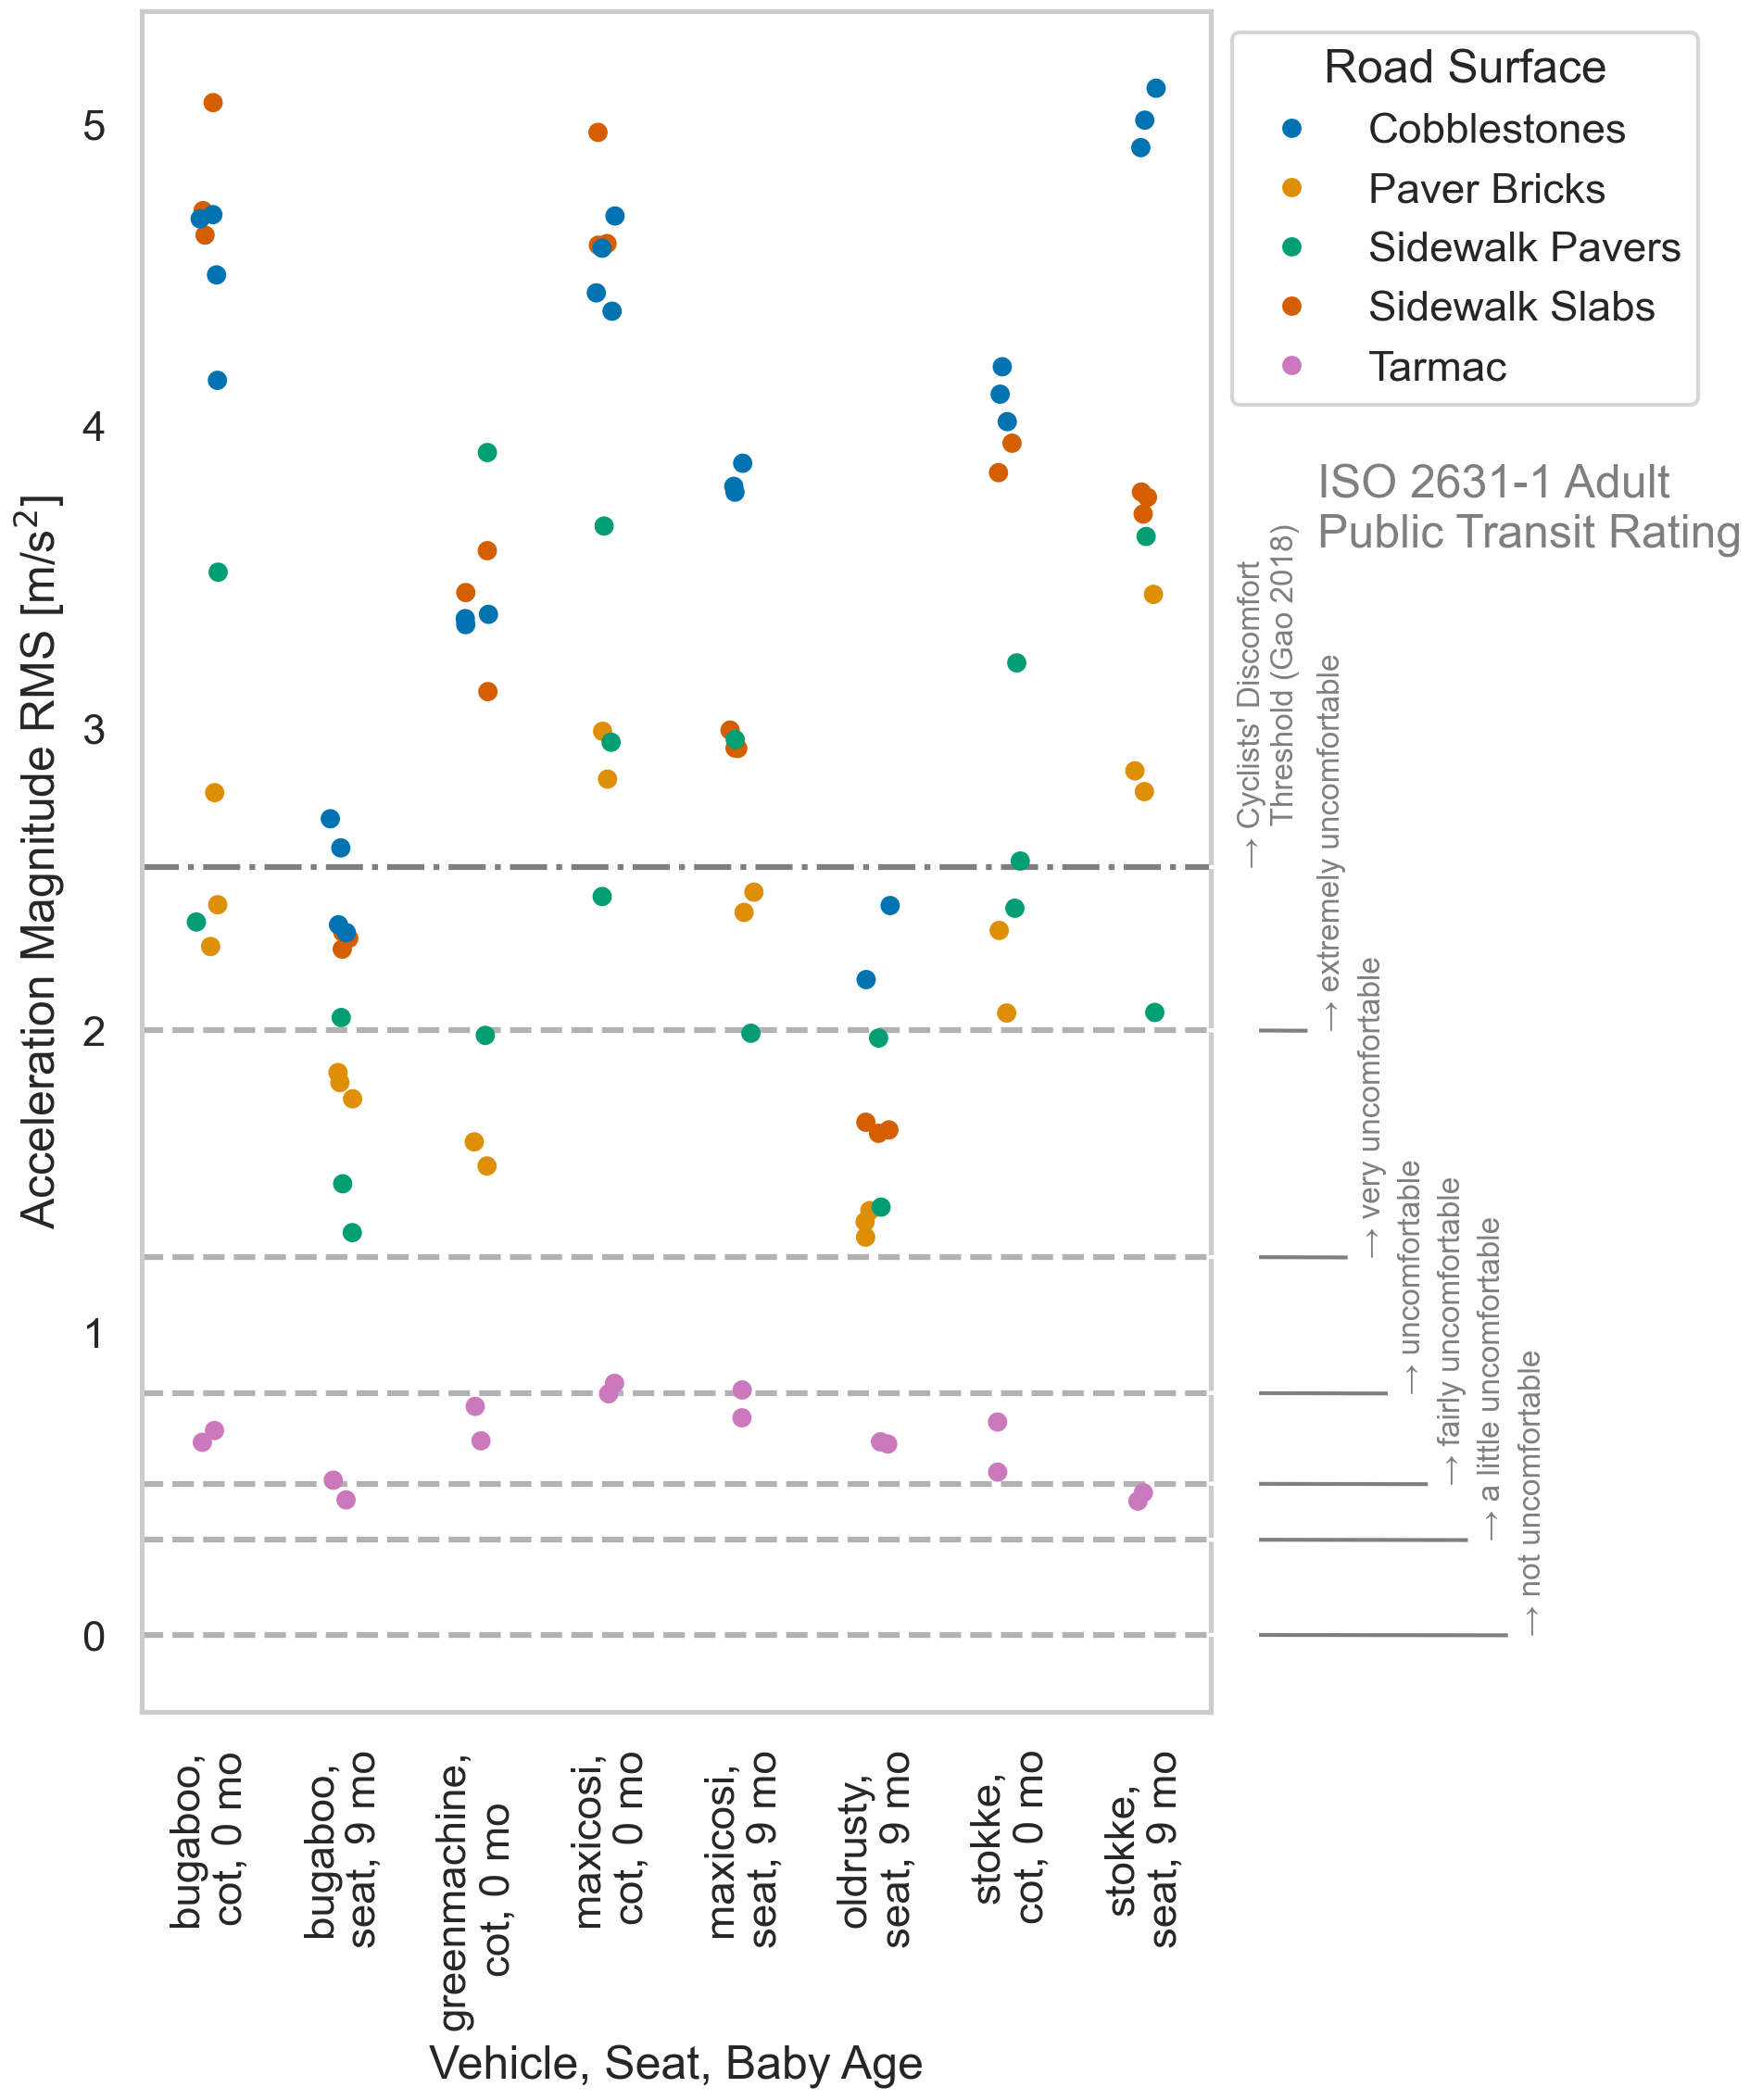
\includegraphics[width=160mm]{fig/SeatBotacc_ver-rms-comfort-stroller-compare-all.png}
  \caption{ISO~2631-1 weighted seat pan magnitude RMS acceleration of all
  stroller repetitions with colour representing road surface. The horizontal
  dashed lines are the lower bound of the ISO~2631-1 ``comfort zones'' for
  adults seated erectly experiencing vibrations in public transit. The
  horizontal dashed dotted line is the cyclists' vibration discomfort threshold
  as reported by Gao et. al~\cite{Gao2018}.}
  \label{fig:comfort-stroller}
\end{figure}

Both of the two cargo bicycles ridden at any tested speed over paver bricks, as
well as the Keiler with the Maxi-Cosi seat ridden over tarmac at high speed fall
into the category ``extremely uncomfortable''. Those are also above the the
cyclist discomfort threshold. The other vehicle setups fall between ``fairly
uncomfortable'' and ``very uncomfortable'' over tarmac for the range of speeds.
The Urban Arrow with the Melia Baby Shell performs, on average, the best on
paver bricks and tarmac at all speeds tested.
%
\begin{figure}
  \centering
  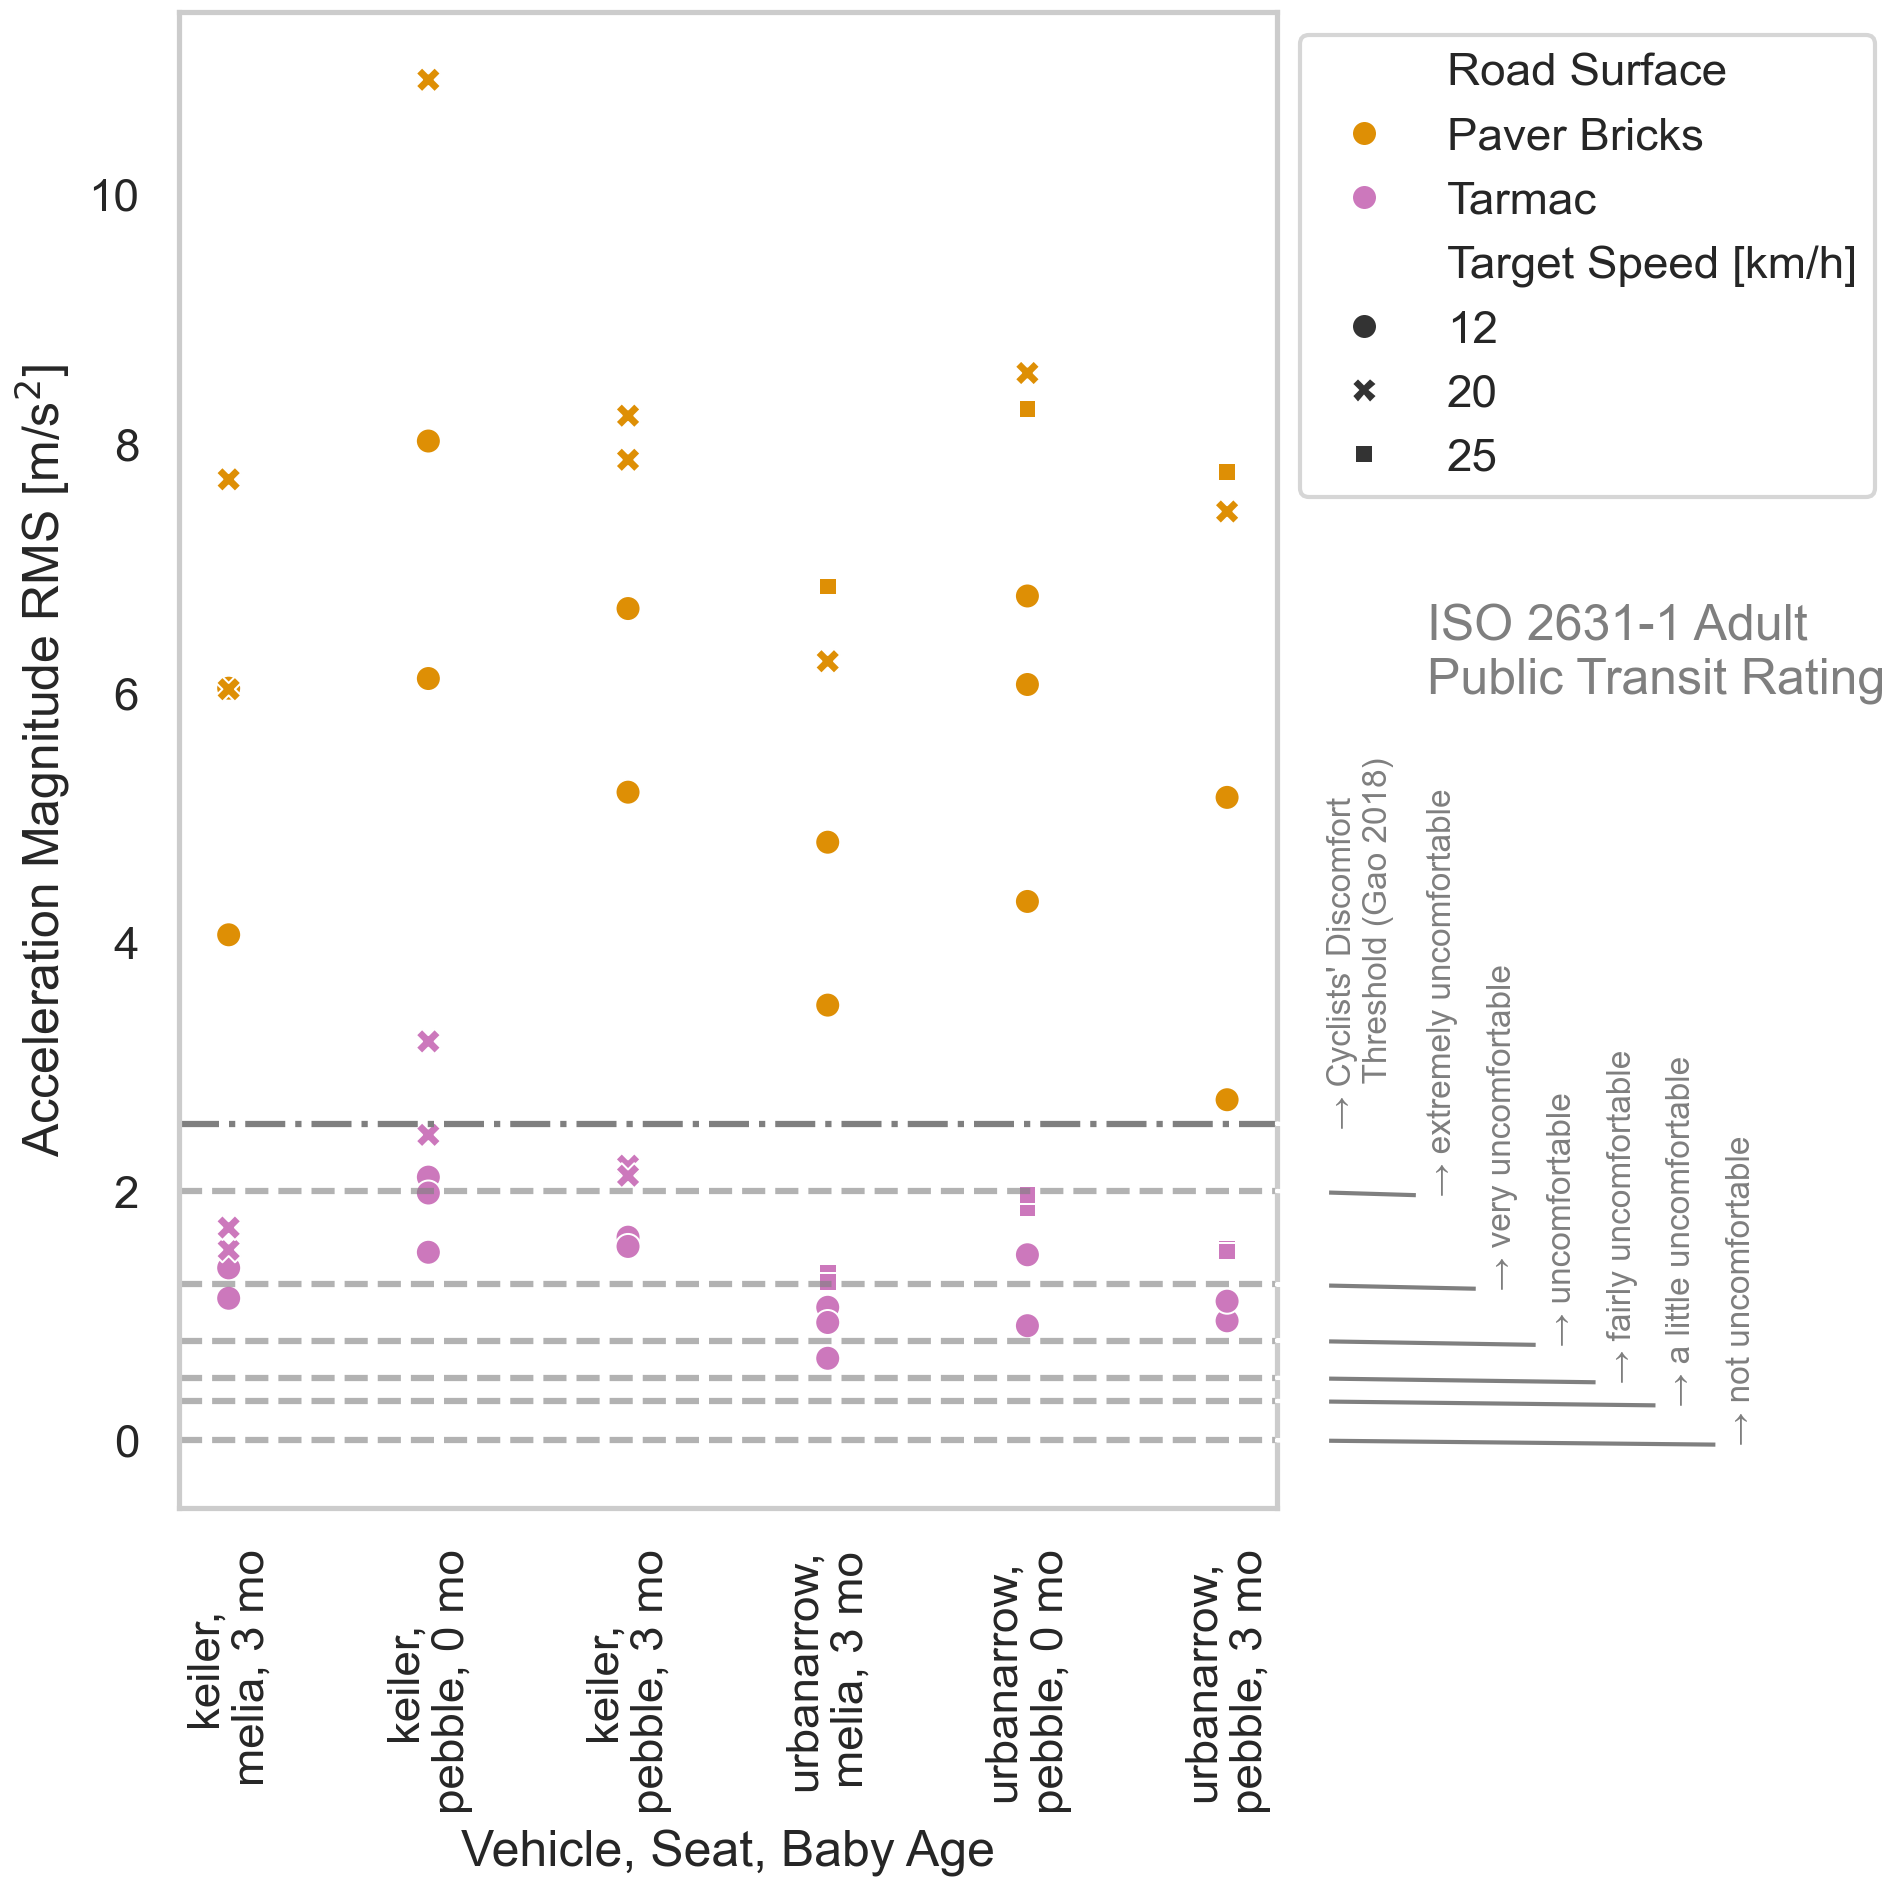
\includegraphics[width=160mm]{fig/SeatBotacc_ver-rms-comfort-bicycle-compare-all.png}
  \caption{ISO~2631-1 weighted seat pan magnitude RMS acceleration of all cargo
  bicycle repetitions with colour representing road surface and marker style
  representing target speed. The horizontal dashed lines with the upper bound of
  the ISO~2631-1 ``comfort zones'' for adults seated erectly experiencing
  vibrations in public transit. The horizontal dashed dotted line is the
  cyclists' vibration discomfort threshold as reported by
  Gao~et.~al~\cite{Gao2018}.}
  \label{fig:comfort-bicycle}
\end{figure}

\subsection{Shock}
%
We identified the maximum peak acceleration values for each trial
(Equation~\ref{eq:max-acc}), then averaged them across repetitions to obtain the
results listed in Table~\ref{tab:shock} for different vehicles and
configurations. There is a significant variation among tests, with the peaks for
the bicycles sometimes reaching the accelerometer's full scale (\(\pm\)16~g).
While the seat pan accelerations for the strollers are generally lower than
those experienced with the bicycles, the configuration (0 or 9 months) may play
a large role. Among bicycles, the use of Melia baby shell seems to transmit
lower accelerations compared to Maxi-Cosi, 3 months, for both the Keiler
tricycle and the Urban Arrow. Strollers with the baby seat configuration for 9
months show much lower acceleration compared to the baby cot for 0 months
(Bugaboo and Maxi-Cosi). Surprisingly, the oldest strollers (Old Rusty and Green
Machine) performed very well during the shock test, resulting in the lowest seat
pan acceleration among all the tested vehicles.
Figure~\ref{fig:shock_vehicle_comparison} shows the peaks of the vertical
acceleration recorded at the seat pan, grouped by different vehicles, for the
shock test. As noted in Table~\ref{tab:shock}, the old strollers Old Rusty and
Green Machine show lower acceleration values. We do not clearly distinguish any
trend with speed for the bicycles (Keiler and Urban Arrow). During the tests
involving Keiler tricycle and strollers, we cannot exclude that the front wheels
(left and right) hit the bump at slightly different time instants.   
%
\begin{figure}
  \centering
  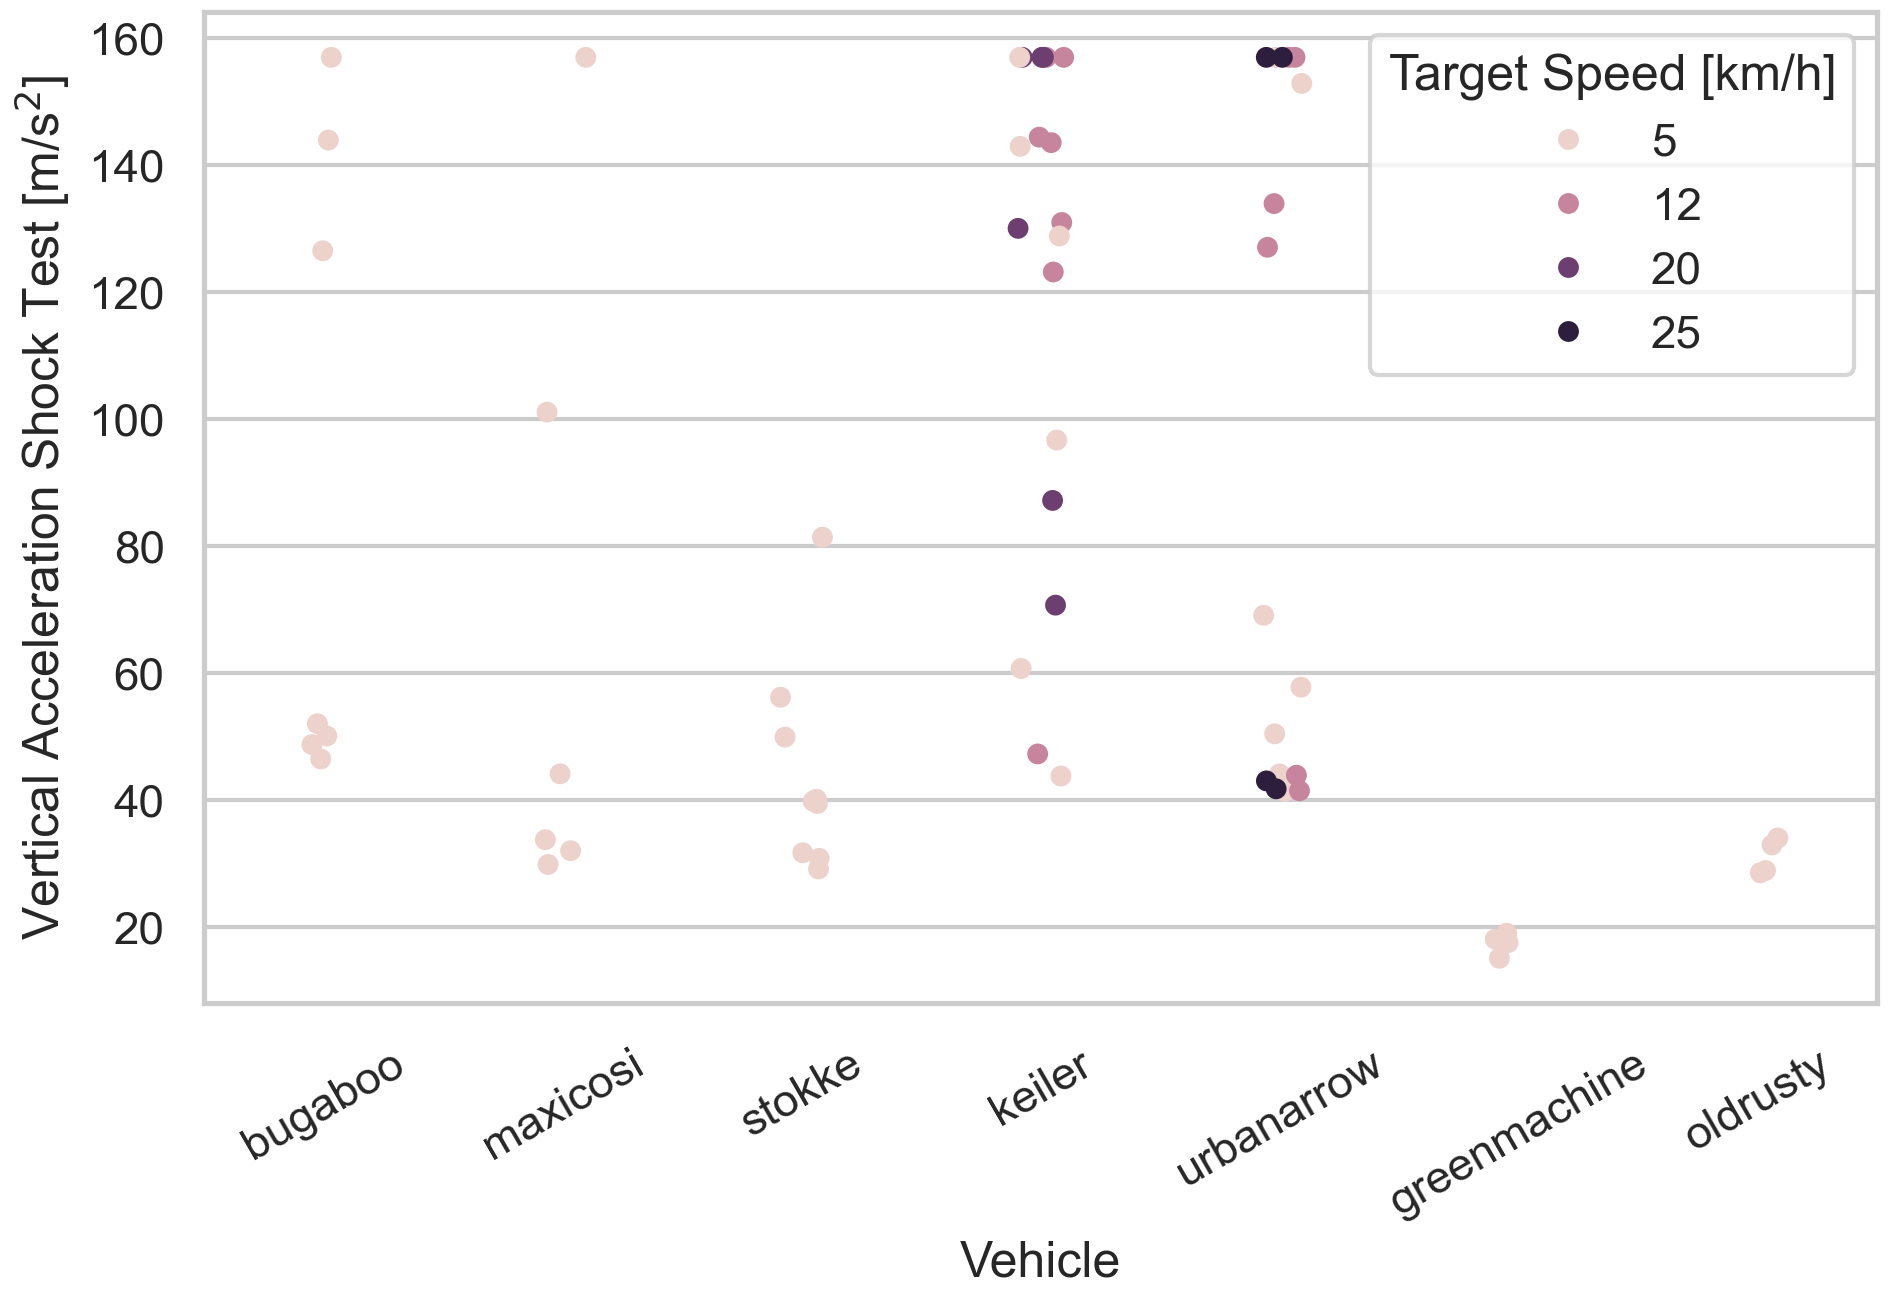
\includegraphics[width=160mm]{fig/SeatBotacc_ver-shock-test-compare.png}
  \caption{Vertical acceleration recorded at the seat pan during the shock test
  per each trial, grouped by vehicles. The colour indicates the mean speed of
  the trial. The lighter the colour the lower the speed.}
  \label{fig:shock_vehicle_comparison}
\end{figure}

\begin{table}
  \centering
  \caption{Mean of the maximum seat pan acceleration across trials in
  \si{\mps\squared} recorded for shock test, for different vehicles and baby
  masses.}
  \label{tab:shock}
  \footnotesize
  \begin{tabular}{lllrrrr}
    \toprule
     & &  & Target Speed & Trial Count & Max Acceleration \\
    Vehicle Type & Model & Seat, Baby & [km/h] & & [m/s²] \\
    \midrule
    Strollers & Bugaboo & Cot, 0 mo  & 5 & 3 & 146 \\
              &         & Seat, 9 mo & 5 & 4 & 49 \\
    \cline{2-6}
              & Maxi-Cosi & Cot, 0 mo  & 5 & 2 & 131 \\
              &           & Seat, 9 mo & 5 & 4 & 35 \\
    \cline{2-6}
              & Stokke BABYZEN YOYO & Cot, 0 mo  & 5 & 4 & 35 \\
              &                     & Seat, 9 mo & 5 & 4 & 51 \\
    \cline{2-6}
              & Green Machine & Cot, 0 mo & 5 & 4 & 17 \\
    \cline{2-6}
              & Old Rusty & Seat, 9 mo & 5 & 4 & 31 \\
    \cline{1-6}
    Bicycles & Keiler tricycle & Melia, 3 mo & 5 & 2 & 52 \\

             &               & Melia, 3 mo & 12 & 2 & 85 \\

             &               & Melia, 3 mo & 20 & 2 & 124 \\
    \cline{2-6}
             &               & Maxi-Cosi, 0 mo & 5 & 2 & 113 \\

             &               & Maxi-Cosi, 0 mo & 12 & 2 & 140 \\

             &               & Maxi-Cosi, 0 mo & 20 & 2 & 115 \\
    \cline{2-6}
             &               & Maxi-Cosi, 3 mo & 5 & 2 & 151 \\

             &               & Maxi-Cosi, 3 mo & 12 & 2 & 160 \\

             &               & Maxi-Cosi, 3 mo & 20 & 2 & 145 \\
    \cline{2-6}
             & Urban Arrow & Melia, 3 mo & 5 & 2 & 43 \\

             &               & Melia, 3 mo & 12 & 2 & 43 \\

             &               & Melia, 3 mo & 25 & 2 & 42 \\
    \cline{2-6}
             &               & Maxi-Cosi, 0 mo & 5 & 1 & 50 \\
    
             &               & Maxi-Cosi, 0 mo & 12 & 2 & 63 \\
    
             &               & Maxi-Cosi, 0 mo & 25 & 2 & 130 \\
    \cline{2-6}
             &               & Maxi-Cosi, 3 mo & 5 & 2 & 156 \\
    
             &               & Maxi-Cosi, 3 mo & 12 & 2 & 160 \\
    
             &               & Maxi-Cosi, 3 mo & 25 & 2 & 160 \\
    \bottomrule
  \end{tabular}
\end{table}

\subsection{Statistical Results}
%
Table~\ref{tab:stroller-ols} shows the results of the 11 degrees of freedom
stroller model for the 104 repetitions~(\(R^2=0.867,F=54.69\)). Both categorical
variables have significant effects. The intercept gives the mean acceleration of
the Green Machine stroller pushed over tarmac, which is not significant. All
road surfaces cause significantly more acceleration than tarmac with
cobblestones having the largest relative effect (3.0~\si{\mps\squared} larger),
followed by sidewalk slabs (2.7~\si{\mps\squared} larger), sidewalk pavers
(1.8~\si{\mps\squared} larger), and paver bricks (1.6~\si{\mps\squared} larger).
The `Bugaboo, Seat, 9 mo' and `Maxi-Cosi, Seat, 9 mo' are not significantly
different than the `Green Machine, Cot, 0 mo' but the other strollers are. The
`Old Rusty, Seat, 9 mo' and `Bugaboo, Cot, 0 mo' showed lower RMS acceleration
than `Green Machine, Cot, 0 mo' by 0.8 and 0.5~\si{\mps\squared}, respectively.
The remaining strollers have larger accelerations than the `Green Machine, Cot,
0 Mo' on tarmac: `Maxi-Cosi, Cot, 0 mo' (1.1~\si{\mps\squared}), `Bugaboo, Cot,
0 mo' (1.0~\si{\mps\squared}), `YOYO, Seat, 9 mo' (1.0~\si{\mps\squared}), and
`YOYO, Seat, 0 mo' (0.6~\si{\mps\squared}).
%
\begin{table}
  \centering
  \caption{Ordinary Linear Regression Results for Stroller. Tarmac and Green
  Machine Cot month are the references for the categorical Road Surface and
  Stroller variables, respectively. The columns give the effect \(\beta\), standard
  error, T-statistic, p-value, and the 95\% confidence interval lower and upper
  bounds.}
  \label{tab:stroller-ols}
  \footnotesize
\begin{tabular}{lcccccc}
\toprule
& \textbf{coef} & \textbf{std err} & \textbf{t} & \textbf{P$> |$t$|$} & \textbf{[0.025} & \textbf{0.975]}  \\
\midrule
\textbf{Intercept}                                                                                     &       0.2212  &        0.188     &     1.177  &         0.242        &       -0.152    &        0.595     \\
Cobblestones                                     &       3.0117  &        0.163     &    18.473  &         0.000        &        2.688    &        3.336     \\
Paver Bricks                                     &       1.6000  &        0.172     &     9.299  &         0.000        &        1.258    &        1.942     \\
Sidewalk Pavers                                  &       1.7566  &        0.174     &    10.092  &         0.000        &        1.411    &        2.102     \\
Sidewalk Slabs                                   &       2.7754  &        0.167     &    16.637  &         0.000        &        2.444    &        3.107     \\
bugaboo, cot, 0 mo   &       0.9706  &        0.202     &     4.813  &         0.000        &        0.570    &        1.371     \\
bugaboo, seat, 9 mo  &      -0.5065  &        0.199     &    -2.551  &         0.012        &       -0.901    &       -0.112     \\
maxicosi, cot, 0 mo  &       1.0795  &        0.202     &     5.353  &         0.000        &        0.679    &        1.480     \\
maxicosi, seat, 9 mo &       0.3012  &        0.209     &     1.441  &         0.153        &       -0.114    &        0.716     \\
oldrusty, seat, 9 mo &      -0.7551  &        0.209     &    -3.605  &         0.001        &       -1.171    &       -0.339     \\
yoyo, cot, 0 mo]     &       0.5766  &        0.209     &     2.753  &         0.007        &        0.161    &        0.993     \\
yoyo, seat, 9 mo     &       0.9706  &        0.205     &     4.731  &         0.000        &        0.563    &        1.378     \\
\bottomrule
\end{tabular}
\end{table}

Table~\ref{tab:bicycle-ols} shows the results of the 8 degree of freedom cargo
bicycle model for the 50 repetitions~(\(R^2=0.925,F=63.17\)). The vehicle setup
categorical variable has significant effects, the road surface categorical
variable alone does not, but the speed and interaction of speed with road
surface do have significant effects. The intercept should theoretically be zero,
because there is no vertical vibration when the speed is zero and the intercept
is not significantly different than zero. Speed is not a significant predictor
on tarmac, but the interaction variable shows that 0.8~\si{\mps\squared} is
gained in acceleration for each 1~\si{\kph} increase on paver bricks. Only the
Urban Arrow with the 3 mo infant in either seat has significant difference to
the `Keiler, Maxi-Cosi, 3 mo', both showing reduction in relative acceleration.
%
\begin{table}
  \centering
  \caption{Ordinary Linear Regression Results for Cargo Bicycle. Tarmac and
  `Keiler, Maxi-Cosi, 3 mo' are the references for the categorical Road Surface
  and Cargo Bicycle variables, respectively. The columns give the effect
  \(\kappa\), standard error, T-statistic, p-value, and the 95\% confidence
  interval lower and upper bounds.}
  \label{tab:bicycle-ols}
  \footnotesize
\begin{tabular}{lcccccc}
\toprule
& \textbf{coef} & \textbf{std err} & \textbf{t} & \textbf{P$> |$t$|$} & \textbf{[0.025} & \textbf{0.975]}  \\
\midrule
\textbf{Intercept}                                                                                          &       0.8067  &        0.643     &     1.255  &         0.216        &       -0.491    &        2.104     \\
Paver Bricks                                          &       1.2956  &        0.889     &     1.457  &         0.153        &       -0.500    &        3.091     \\
keiler, maxicosi, 0 mo     &       0.8664  &        0.415     &     2.085  &         0.043        &        0.027    &        1.705     \\
keiler, melia, 3 mo        &      -0.5060  &        0.415     &    -1.219  &         0.230        &       -1.344    &        0.332     \\
urbanarrow, maxicosi, 0 mo &      -0.0512  &        0.404     &    -0.127  &         0.900        &       -0.867    &        0.764     \\
urbanarrow, maxicosi, 3 mo &      -0.8895  &        0.415     &    -2.141  &         0.038        &       -1.728    &       -0.051     \\
urbanarrow, melia, 3 mo    &      -1.1357  &        0.403     &    -2.819  &         0.007        &       -1.949    &       -0.322     \\
Mean Speed [m/s]                                                                              &       0.2034  &        0.116     &     1.747  &         0.088        &       -0.032    &        0.439     \\
Mean Speed\(\times\)Road Surface                    &       0.7803  &        0.180     &     4.338  &         0.000        &        0.417    &        1.144     \\
\bottomrule
\end{tabular}
  \end{table}
  
\paragraph{Vehicle Comparisons}
%
Given that the vehicle setup (\(x_\textrm{Stroller}\) and \(x_\textrm{Cargo
Bicycle}\)) is a significant effect, we perform a post-hoc analysis to compare
vehicles on each road surface. Table~\ref{tab:sig-group-stroller}, derived from
Figure~\ref{fig:tukey-stroller} in Appendix~\ref{app:compare}, shows the
groupings of non-significant comparisons for a Tukey Range Test among the
strollers.
Old Rusty and `Bugaboo, Seat, 9 mo' and the Green Machine perform generally
better (significantly) than the other vehicles, shown by the ``overall''
ranking.
For cobblestones, this is also true as well as: 1) the `YOYO, Seat, 9 mo' is the
worst stroller tested and, interestingly, the the heavier dummy performs worse
than the lighter dummy, 2) the 9 mo dummy experiences less acceleration in the
Bugaboo and Maxi-Cosi.
For paver bricks: 1) Old Rusty, `Bugaboo, Seat, 9 mo', and Green Machine are
again the best and 2) `YOYO, Seat, 9 mo' sees more acceleration than the 0 mo
configuration.
For sidewalk pavers, there is no significant difference among the strollers.
For side walk slabs: 1) Old Rusty is the best and Bugaboo the second best,
2) the 0 month in the Bugaboo and Maxi-Cosi see more than the 9 month in the
same vehicle, respectively, and 3) no difference in the YOYO when comparing
dummy sizes.
For tarmac: the Green Machine, `Bugaboo, Seat, 9 mo', and `YOYO, Seat, 9 mo' are
better than Maxi-cosi with either dummy size and 2) the Green Machine is better
than the `Bugaboo, Cot, 0 mo'.
%
\begin{table}
\centering
\caption{Stroller Significance Ranking Groups (based on
Figure~\ref{fig:tukey-stroller}). The numbers indicate the group where there is
no significant difference with 1 being the best (lower acceleration) and 8 being
the worst (higher acceleration). The ``Overall'' column gives an overall ranking
based on the mean ranking of the other columns.}
\label{tab:sig-group-stroller}
\begin{tabular}{lcccccc}
  \toprule
                          &         &              & Paver  & Sidewalk & Sidewalk & \\
  Vehicle Setup           & Overall & Cobblestones & Bricks & Pavers   & Slabs    & Tarmac \\
  \midrule
  yoyo, seat, 9 mo        & 7 & 8   & 6-8 & 1-8 & 5-6 & 1-6 \\
  yoyo, cot, 0 mo         & 4 & 4-5 & 3-5 & 1-8 & 5-6 & 1-8 \\
  oldrusty, seat, 9 mo    & 1 & 1-2 & 1-3 & 1-8 & 1   & 1-8 \\
  maxicosi, seat, 9 mo    & 4 & 4-5 & 3-6 & 1-8 & 3-4 & 4-8 \\
  maxicosi, seat, 0 mo    & 8 & 6-7 & 6-8 & 1-8 & 7-8 & 4-8 \\
  greenmachine, cot, 0 mo & 3 & 3   & 1-3 & 1-8 & 3-4 & 1-4 \\
  bugaboo, seat, 9 mo     & 1 & 1-2 & 1-3 & 1-8 & 2   & 1-6 \\
  bugaboo, cot, 0 mo      & 6 & 6-7 & 3-6 & 1-8 & 7-8 & 2-8 \\
  \bottomrule
\end{tabular}
\end{table}

When comparing the cargo bicycles, Table~\ref{tab:sig-group-bicycle}, most
vehicle setups deliver similar acceleration to the seat pan when ridden over the
same surface at the same target speed. For low speed on tarmac, the Urban Arrow
with the Meila Baby Shell and a 3 mo dummy has significantly less acceleration
than the Keiler with the Maxicosi and 0 mo dummy. There is no significant
difference in any vehicle setups at low speed on paver bricks. At higher speeds,
the Urban Arrow and Keiler with the Meila seat and the 3 mo dummy is
significantly better than the Keiler with the Maxicosi and the 0 mo on paver
bricks and on tarmac. It is important to point out that there is no significant
difference when simply swapping the seat for the 3 mo dummy, which does not
support the hypothesis in Section~\ref{sec:health-assesment}.
%
\begin{table}
\centering
\caption{Cargo Bicycle Significance Ranking Groups (based on
Figure~\ref{fig:tukey-bicycle}). The numbers indicate the group where there is
no significant difference with 1 being the best (lower acceleration) and 6 being
the worst (higher acceleration). The ``Overall'' column gives an overall ranking
based on the mean ranking of the other columns. Note that the mean ranking is
very close for all cargo bicycles.}
\label{tab:sig-group-bicycle}
\begin{tabular}{lccccc}
     \toprule
                                &         & Paver Bricks & Tarmac    & Paver Bricks & Tarmac \\
     Vehicle Setup              & Overall & Low Speed    & Low Speed & High Speed   & High Speed \\
     \midrule
     urbanarrow, melia, 3 mo    & 1 & 1-6 & 1-5 & 1-5 & 1-5\\
     urbanarrow, maxicosi, 3 mo & 2 & 1-6 & 1-6 & 1-5 & 1-5\\
     urbanarrow, maxicosi, 0 mo & 4 & 1-6 & 1-6 & 1-6 & 1-5\\
     keiler, melia, 3 mo        & 2 & 1-6 & 1-6 & 1-5 & 1-5\\
     keiler, maxicosi, 3 mo     & 5 & 1-6 & 1-6 & 1-6 & 1-6\\
     keiler, maxicosi, 0 mo     & 6 & 1-6 & 2-6 & 3-6 & 4-6\\
     \bottomrule
\end{tabular}
\end{table}

\section{Discussion}
%
We have presented a comprehensive set of acceleration measurements from
experiments that simulate the vibrations experienced by dummy infants in the 0-9
month mass range during transportation in both strollers and cargo bicycles. We
compared the average magnitude of vertical and total acceleration at the seat
pan across a variety of road surfaces and seats while moving at typical vehicle
travel speeds. Excluding the shock tests, ISO~2631-1 weighted average
acceleration can range from \SIrange{0.4}{10.7}{\mps\squared} across all tested
scenarios. Strollers induced \SIrange{0.4}{5.0}{\mps\squared} average
acceleration for a mean walking speed of 5.3~\si{\kph}. Cargo bicycles induced
\SIrange{0.6}{10.7}{\mps\squared} over a speed range of \SIrange{12}{25}{\kph}.

\subsection{Surface and Speed}
%
Travelling over a tarmac surface offers the least vibration to all vehicle types
at any speed with a maximum average acceleration of
1.2~\si{\meter\per\second\squared}. For strollers, travelling over surfaces
rougher than tarmac at normal walking speed can cause, on average, 5\(\times\)
the acceleration experienced on tarmac with average accelerations reaching
5.0~\si{\meter\per\second\squared}. Cobblestones and the large gaps in the
sidewalk slabs caused the largest magnitude of vibrations at the seat pan in the
strollers. Cobblestones and sidewalk slabs approximately double the vibration
amplitude relative to sidewalk paver and paver bricks, with them all being
significant larger than tarmac vibrations.

For cargo bicycles, travelling over paver bricks at the same speeds can
quadruple the magnitude of the average acceleration the dummy experiences.
Travelling at the maximum allowed speed of an electric cargo bicycle (25
\si{\kph}) over paver bricks caused the dummy to experience average
accelerations exceeding 8~\si{\mps\squared}. The effect of speed on vibration is
significant for paver bricks but not for tarmac. 

Whereas speed strongly affected the acceleration amplitude it does not strongly
affect the peak frequency and the bandwidth below which 80\% of power is
contained. This suggests that peak frequencies represent oscillations induced by
the systems tested rather than dominant frequencies resulting from the road
surface.

\subsection{Baby Mass}
%
The size of the dummy (mass and build) had no obvious and systematic effect on
the average acceleration at the seat pan body-seat interface. These vibrations
are transmitted to an infant's body and the physical properties (mass,
stiffness, damping) of the infant's body determine whether this excitation is
amplified or not and which body segment is more affected. Tests with more
realistic dummies or real infants are necessary to investigate how the infant
itself moves when excited by this level of vibration. This information is not
readily available in the literature and may be hard to acquire due to ethical
limitations and the absence of validated infant dummies. The only effect that
stood out for mass was that, counter-intuitively, the lighter dummy has less
acceleration than the heavier dummy for the Stokke BABYZEN YOYO 0+ stroller.

\subsection{Health}
%
The vibrations measured in the different scenarios showed that RMS acceleration
can be relatively large when compared to the smoothest experience on tarmac.
There is a large gap in the literature connecting acceleration magnitude to
discomfort and/or health consequences, which is particularly absent for infants.
The most used health and comfort assessment tool for whole-body vibration is the
ISO~2631-1 standard. When we investigated health risks using the standard we
found that:
%
\begin{itemize}
    \item only strollers pushed over tarmac at 5~\si{\kph} had average
    acceleration below the ``health risk zone" for 4~\si{\hour} daily duration,
    \item strollers pushed over cobblestones and sidewalk slabs can deliver
    accelerations in the ``health risk zone'' with durations less than
    20~\si{\min},
    \item cargo bicycles ridden at \SIrange{12}{25}{\kph} over tarmac
    overwhelmingly delivered accelerations below the 1~\si{\hour} ``health risk
    zone'', and
    \item cargo bicycles ridden at \SIrange{12}{25}{\kph} over paver bricks
    delivered accelerations well into the 10~\si{\min} ``health risk zone''.
\end{itemize}
%
When we compare the vibration we measured for infants in strollers and cargo
bicycles with the vibration ``health risk zone'' as defined for adults in the
ISO~2631-1 standard, we see that:
%
\begin{itemize}
    \item cycling with an infant in a cargo bicycle on paver bricks with
    20~\si{\kph} for 10~\si{\min} gives the infant a vibration load that equals
    or exceeds the ``health risk zone'' for adults seated erectly experiencing
    vibrations,
    \item cycling with an infant in a cargo bicycle on tarmac at 12~\si{\kph} can
    be maintained for approximately two hours before exceeding the ``health risk
    zone'' for adults seated erectly experiencing vibrations,
    \item walking with an infant in a stroller on cobblestones can exceed the
    ``health risk zone'' for adults seated erectly experiencing vibrations
    within 15~\si{\min} to 1~\si{\hour}, depending on the stroller model and the
    age of the child, and
    \item walking with an infant in a stroller on tarmac can be continued for
    four hours without exceeding the ``health risk zone'' for adults seated
    erectly experiencing vibrations.
\end{itemize}
    
We can conclude that strollers can be pushed over paver bricks and sidewalk
pavers continuously for maximal about half an hour. On extreme surfaces like
cobblestones and sidewalk slabs, strollers should be pushed slower than
5~\si{\kph} with a duration of maximal 10~\si{\min}. Only on tarmac a stroller
can be walked continuously for four hours (but only if the infant is in the cot,
for if it is sitting it needs appropriate breaks to enable movement). Cargo
bicycles carrying infants over paver bricks should slow down to 12~\si{\kph} or
preferably less and the duration should be kept under 10~\si{\min}. When riding
a cargo bicycle over tarmac at 20\si{\kph}, the duration should be kept under
1~\si{\hour}. At 12~\si{\kph} cargo bicycles can ride over tarmac for maximal
2~\si{\hour}.

\subsection{Comfort}
%
When considering comfort, the ISO~2631-1 guidelines indicate that adults would
report the vibrations experienced in strollers and bicycles as uncomfortable.
For strollers, the vibrations over tarmac would be rated ``fairly
uncomfortable'' and all other road surfaces would be ``very'' or ``extremely
uncomfortable''. When riding a cargo bicycle over paver bricks, the vibrations
would be rated as ``extremely uncomfortable'' and over tarmac spans ``fairly``
to ``extremely''. The ISO~2631-1 comfort rating scale is derived from adult
subjective ratings of vibrations felt when riding public transit for an
unspecified duration, so this scale is unlikely appropriate to apply for our
situation. Gao~et~al.~\cite{Gao2018} reports that cyclists do not rate
vibrations as extremely uncomfortable on normal road surfaces, indicating some
contradiction.

\subsection{Vehicle and Seat Design}
%
Different vehicle, seat, and baby mass combinations cause different average
vertical accelerations at the seat pan. We are only able to compare vehicle
setup to vehicle setup, other than comparing the same two different baby seats
in both cargo bikes. A striking discovery is that the two 1970's strollers we
tested were significantly better than many of the modern stroller setups on most
road surfaces. The vintage strollers actually had more sophisticated suspension
systems that used springs, straps, and mechanisms, and they also had larger
wheels. Stroller manufacturers may have reduced suspension as a side effect to
decreasing the size and weight of strollers and introducing swivelling front
wheels (which makes steering lighter but can technically not be combined with
the design of old suspension types). As an example, the ``Old Rusty'' stroller
was the only one that did not exceed the 1~\si{\hour} health risk line for all
road surfaces.

Both the Bugaboo Fox 5 and Maxi-Cosi Street Plus stroller showed lower
acceleration for the heavier baby, as expected, but the Stokke BABYZEN YOYO 0+
showed the opposite trend for cobblestones and paver bricks. This points to
design choices that may cause resonance on certain surface profiles. The
`Bugaboo, Seat, 9 mo' configuration performed better than the other modern
strollers for all non-tarmac road surfaces. Urban Arrow performed better than
Keiler on tarmac but there is no difference on paver bricks. Additionally, there
was no difference in the different seats for the 3 month infant. Performance of
a vehicle setup is not necessarily constant with respect to cot or seat
configuration, contrarily, performance is often significantly different when
converting for different baby ages. This points towards designs that are only
optimized for one configuration.

\subsection{ISO Filters and Bandwidth}
%
We report RMS accelerations up to 120~\si{\hertz} Hz as well as accelerations
weighted according to the ISO standards for vibration (VDV). Vibrations at
frequencies between \SIrange{4.9}{10.7}{\hertz} showed to have the largest
magnitude contribution to the vibrations, but there is a frequency content of
magnitudes of interest in a bandwidth of up to 45~\si{\hertz}. Our results show
substantial differences between RMS and VDV highlighting the importance of
reviewing their meaning. These differences emerge from the high bandwidth of the
accelerations now measured, which greatly exceed the bandwidth of accelerations
measured with adults seated in cars (see e.g Figure 2 in
\cite{griffin2004experimental}). Adult experiments show that significant
discomfort can be measured across all tested frequencies being 80 Hz
\cite{morioka2010frequency} or even 315~\si{\hertz}~\cite{morioka2006magnitude}
albeit with reduced sensitivity.

The ISO frequency weightings are defined for adults in more or less erect
postures with the head being unsupported, whereas we now studied dummies
representing infants from 0-9 months lying with the head directly supported. The
ISO~2631-1 weightings represent a reduced sensitivity above 8~\si{\hertz}, which
is associated with the vertical dynamics of erect seated subjects which filter
out such high frequencies \cite{toward2011transmission,mirakhorlo2022effects}.
However, adult experiments show higher discomfort for frequencies above
8~\si{\hertz} when lying with head supported with \SIrange{30}{90}{\degree} back
inclination as compared to erect without head support. Higher frequencies have
also been associated with effects on the central nervous system. For instance,
experiments on rats showed brain injury visible in behaviour through functional
impairment and in visual changes of brain structures in postmortem dissection
after exposure to prolonged whole-body vibration at 30~\si{\hertz} and
5~\si{\mps\squared}~\cite{Yan2015_cumulative_brain_injury/j.jstrokecerebrovasdis.2015.08.007}.
In some conditions, the RMS exceeds the ISO Weighted RMS substantially,
warranting further research on the effects of higher frequencies in particular
for head supported conditions and for children. The VDV showed even higher
values warranting further research on the relevance of peaks and transients.

\section{Conclusion}
%
\subsection{Summary}
%
The results herein raise concerns about transporting infants in strollers and
cargo bicycles. If the user's behaviour is not adjusted to avoid rough surfaces
or to go very slow over them when the cargo is an infant, there are potential
health risks if the large vibrations are experienced daily and repeatedly over a
longer time. In most likelihood, users do adjust their travel behaviour, but
maybe not enough or possibly they are neglectful, but this has yet to be
studied. There is no direct evidence that connects whole-body vibration as
measured in this study to infant harm or negative health effects, so we can only
extrapolate from the limited guidelines on adults in occupational settings. But
we did measure vibrations that would not be permitted for adults to maintain
long term occupational health and it is reasonable to believe we should not
subject our infants to the same.

It is well known that whole-body vibration can be controlled with good
suspension design. We see this in the drastic historical evolution of suspension
in automobiles. We do not see this same kind of attention to suspension in
strollers, cargo bicycles, and baby seats for these vehicles. Walking and
cycling is well known to offer great societal and personal benefits over
travelling by car, so it behoves us all to make transport for infants most
optimal in these two transport modes. 

\subsection{Recommendations}
%
Our conclusions result primarily from the recommended application of ISO~2631-1.
It is of utmost importance to recognize that this standard cautions extending
the use of the standard to situations of which its supporting data was not
derived. The standard is based primarily on pre-1997 studies of adult whole-body
vibration in occupational durations (\SIrange{4}{8}{\hour} daily dose) or during
public transportation.
%
\begin{quote}
  \textbf{The recommendations in standard ISO~2631-1 have not been based on or validated for: 1)
  short durations that dominate stroller and cargo bicycle travel, 2) infants,
  children, or young adults, 3) nor to recumbent or reclined seating postures with the head supported.
  So our recommendations must be taken with utmost caution, at least until more
  research is done to improve the standard guidance.}
\end{quote}
%
Nevertheless, the following list provides recommendations for users,
researchers, designers, and manufacturers based on the findings of this paper
that we believe stand in spite of the standard's limitations:
%
\begin{enumerate}
    \item Stroller, cargo bicycle, and seat manufacturers should test for
    vibration for all expected surface types and ranges of relevant body sizes
    and posture to ensure their designs isolate vibrations well for all use
    conditions. Testing across relevant body sizes is especially important for
    strollers, due to the high mass of the infant relative to the stroller mass.
    \item Manufacturers should collaborate in testing and report their results
    publicly, similar to the automobile industry safety ratings. For the
    combined use of cargo bicycles and baby seats, manufacturers should
    collaborate in this effort.
    \item Manufacturers and scientists should collaborate to develop metrics and
    testing procedures for the long-term goal of a new standard.
    \item Designers should ensure that adequate vibration isolation occurs for
    vehicles that have multiple configurations (e.g. recumbent vs. erect
    seating).
    \item Designers and manufacturers should incorporate better suspension
    systems, as currently occurring vibrations can be drastically reduced.
    Useful information may be derived from past designs with better suspension.
    \item Cycling roads should have a tarmac-like smoothness. Cobblestones
    should be avoided.
    \item Sidewalks should have a tarmac-like smoothness. Cobblestones should be
    avoided for strollers.
    \item Users should limit their speed when walking with strollers or riding
    over surfaces rougher than tarmac, as bumpier surfaces can quickly multiply
    the experienced accelerations.
    \item Users are suggested to limit the duration of transport over surfaces
    rougher than tarmac to periods that do not exceed 10-30 continuous minutes
    depending on the system (existence of suspension, larger tyres or wheels)
    and other countermeasures like adequate non-vibration breaks in between.
    When transporting over tarmac, continuous durations should not exceed
    4~hours and need to include regular breaks, if only to give the infant
    opportunity to move.
    \item Preferably ride any cargo bicycle at a speed of maximal 12~\si{\kph}
    over surfaces rougher than tarmac. E-cargo bicycles can easily reach the
    maximum speed of 25~\si{\kph}. Infants should only be transported for short
    durations when riding over non-tarmac surfaces at these speeds.
    \item Standard ISO~2631-1 is not based on or validated to characterize
    health and comfort effects of vibration for infants or children or for short
    durations or non-erect seating. However, this is the only available standard
    in the literature assessing health and comfort levels on vibrations, and
    could be used as benchmark.
\end{enumerate}

\subsection{Future Work}
% 
There are four possible directions for future work: more in-depth analysis of
the present measurements, more research on vibrations generated by infant
transport systems, more research on the effects of vibration on infants, and
development of a benchmark.

\paragraph{Concerning further analysis of the present measurements:}
%
We acquired data from four other sensors on the vehicles, each with three
accelerometer and three gyroscope time histories, for a total of 30 time
histories of possible interest. This paper provides a look into the experiments
via four metrics: ISO weighted vertical RMS acceleration, maximum acceleration,
peak frequency, and bandwidth of the seat pan sensor. The collected data can
also be used to investigate the transmissibility from sensor to sensor, as well
as rotational vibration effects. Investigating these further can give a more
complete picture of the connections to health and comfort. This work also gives
a benchmark against which new designs can be tested to show reduction in
vibration.

\paragraph{Concerning more research on vibrations generated by infant transport
systems:}
%
There are products and variables that have not yet been investigated for their
effect on vibration. For example, running with an infant in a sports stroller is
not tested. Investigating this is important because we expect that vibrations
when running may quickly exceed health limits. In addition, recumbent posture in
sports strollers is estimated to increase the vibration load on the head of the
infant. It is important to establish the actual vibration load on the head in
practice.

\paragraph{Concerning more research on the effects of vibration on infants:}
%
The frequency weighting of the ISO~2631-1 standard is not designed or validated
to characterise health and comfort for infants or children, for short durations,
and for non-erect seating. Research is urgently needed to develop a new standard
with a more appropriate frequency weighting to improve assessment of the comfort
and health effects of whole-body vibration of infants and children, also for
short durations and for non-erect seating. Furthermore, tests with more
realistic dummies and/or real infants are necessary to investigate how the
infant itself moves when excited by various vibrations in different postures.
The results will contribute to the assessment of the transmissibility of
vibration in children, which is needed to deduce the vibrations transmitted to
the head. 

\paragraph{Concerning the development of a benchmark:}
%
At this moment, no requirements are made for the vibrational properties of child
transport systems in the standards for strollers, cargo bicycles, bicycle seats,
and car seats. Due to the magnitude of vibrations that can occur during child
transport, it is imperative to include a requirement to the vibrational
properties in the standards for these products. At this moment, no new
requirements can be defined because there is not enough information. With the
information resulting from more research on infant vibration, a benchmark for
the vibration properties of infant transportation products needs to be
developed. This will enable the inclusion of minimal requirements for vibration
properties in the standards, which would greatly increase the health and comfort
of the infants who must use these products. 

\subsection{Acknowledgement}
%
We acknowledge the advice and financial support of VeiligheidNL.

\bibliographystyle{plain}
\bibliography{reference}

\newpage
\appendix

% Ensure subsections retain "A.1", "A.2", etc.
%\addcontentsline{toc}{section}{Appendix} % Optional: Add to TOC
%\renewcommand{\thesection}{A}
%\renewcommand{\thesubsection}{\thesection.\arabic{subsection}}

\section{Experimental Equipment}
\label{app:equipment}
%
In this section, we report the pictures of the strollers and bicycles used for
the experiments. The reader can find the measurements, wheelbase, wheel
diameter, sensor location and orientation for all the tested vehicles.

\begin{figure}[htbp]    % use [htbp] to place the figures where I prefer
  \centering
  \subcaptionbox{Lateral view}{\includegraphics[width=75mm]{fig/TechDraw_UA-Joolz_lat.pdf}}
  \subcaptionbox{Front view}{\includegraphics[width=80mm]{fig/TechDraw_UA-Joolz_front.pdf}}
  \caption{IMU locations on the Urban Arrow cargo bicycle, equipped with the
  Maxicosi-Joolz baby Pebble.}
  \label{fig:tech_drawing_UA_Joolz}
\end{figure}

\begin{figure}[htbp]    % use [htbp] to place the figures where I prefer
  \centering
  \subcaptionbox{Lateral view}{\includegraphics[width=75mm]{fig/TechDraw_UA-Melia_lat.pdf}}
  \subcaptionbox{Front view}{\includegraphics[width=80mm]{fig/TechDraw_UA-Melia_front.pdf}}
  \caption{IMU locations on the Urban Arrow cargo bicycle, equipped with the
  Melia baby shell.}
  \label{fig:tech_drawing_UA_Melia}
\end{figure}

\clearpage
\begin{figure}[htbp]
  \centering
  \subcaptionbox{Lateral view}{\includegraphics[width=75mm]{fig/TechDraw_Trike-Joolz_lat.pdf}}
  \subcaptionbox{Front view}{\includegraphics[width=80mm]{fig/TechDraw_Trike-Joolz_front.pdf}}
  \caption{IMU locations on the Keiler Tricycle, equipped with the
  Maxicosi-Joolz baby pebble.}
  \label{fig:tech_drawing_Trike_Joolz}
\end{figure}


\begin{figure}[htbp]
  \centering
  \subcaptionbox{Lateral view}{\includegraphics[width=75mm]{fig/TechDraw_Trike-Melia_lat.pdf}}
  \subcaptionbox{Front view}{\includegraphics[width=75mm]{fig/TechDraw_Trike-Melia_front.pdf}}
  \caption{IMU locations on the Keiler Tricycle, equipped with the
  Melia baby shell.}
  \label{fig:tech_drawing_Trike_Melia}
\end{figure}

\clearpage
\begin{figure}[htbp]
  \centering
  \subcaptionbox{Lateral view}{\includegraphics[width=70mm]{fig/TechDraw_Bugaboo0_lat.pdf}}
  \subcaptionbox{Front view}{\includegraphics[width=70mm]{fig/TechDraw_Bugaboo0_front.pdf}}
  \caption{IMU locations on the stroller Bugaboo Fox 5, configured for 0-months baby.}
  \label{fig:tech_drawing_Bugaboo0}
\end{figure}

\begin{figure}[htbp]
  \centering
  \subcaptionbox{Lateral view}{\includegraphics[width=70mm, angle=-90]{fig/TechDraw_Bugaboo9_lat.pdf}}
  \subcaptionbox{Front view}{\includegraphics[width=70mm]{fig/TechDraw_Bugaboo9_front.pdf}}
  \caption{IMU locations on the stroller Bugaboo Fox 5, configured for 9-months baby.}
  \label{fig:tech_drawing_Bugaboo9}
\end{figure}

\clearpage
\begin{figure}[htbp]
  \centering
  \subcaptionbox{Lateral view}{\includegraphics[width=70mm, angle=-90]{fig/TechDraw_Maxicosi0_lat.pdf}}
  \subcaptionbox{Front view}{\includegraphics[width=70mm]{fig/TechDraw_Maxicosi0_front.pdf}}
  \caption{IMU locations on the stroller Maxi-Cosi Street Plus, configured for 0-months baby.}
  \label{fig:tech_drawing_Maxicosi0}
\end{figure}

\begin{figure}[htbp]
  \centering
  \subcaptionbox{Lateral view}{\includegraphics[width=70mm, angle=-90]{fig/TechDraw_Maxicosi9_lat.pdf}}
  \subcaptionbox{Front view}{\includegraphics[width=70mm,angle=-90]{fig/TechDraw_Maxicosi9_front.pdf}}
  \caption{IMU locations on the stroller Maxi-Cosi Street Plus, configured for 9-months baby.}
  \label{fig:tech_drawing_Maxicosi9}
\end{figure}

\clearpage
\begin{figure}[htbp]
  \centering
  \subcaptionbox{Lateral view}{\includegraphics[width=70mm, angle=-90]{fig/TechDraw_YOYO0_lat.pdf}}
  \subcaptionbox{Front view}{\includegraphics[width=70mm]{fig/TechDraw_YOYO0_front.pdf}}
  \caption{IMU locations on the stroller Stokke BABYZEN YOYO 0+, configured for 0-months baby.}
  \label{fig:tech_drawing_YOYO0}
\end{figure}

\begin{figure}[htbp]
  \centering
  \subcaptionbox{Lateral view}{\includegraphics[width=70mm, angle=-90]{fig/TechDraw_YOYO9_lat.pdf}}
  \subcaptionbox{Front view}{\includegraphics[width=70mm]{fig/TechDraw_YOYO9_front.pdf}}
  \caption{IMU locations on the stroller Stokke BABYZEN YOYO 0+, configured for 9-months baby.}
  \label{fig:tech_drawing_YOYO9}
\end{figure}

\clearpage
\begin{figure}[htbp]
  \centering
  \subcaptionbox{Lateral view}{\includegraphics[width=70mm, angle=-90]{fig/TechDraw_GreenM0_lat.pdf}}
  \subcaptionbox{Front view}{\includegraphics[width=70mm]{fig/TechDraw_GreenM0_front.pdf}}
  \caption{IMU locations on the old stroller Green Machine, configured for 0-months baby.}
  \label{fig:tech_drawing_GreenM0}
\end{figure}

\begin{figure}[htbp]
  \centering
  \subcaptionbox{Lateral view}{\includegraphics[width=70mm, angle=-90]{fig/TechDraw_OldR9_lat.pdf}}
  \subcaptionbox{Front view}{\includegraphics[width=70mm]{fig/TechDraw_OldR9_front.pdf}}
  \caption{IMU locations on the old stroller Old Rusty, configured for 9-months baby.}
  \label{fig:tech_drawing_OldR9}
\end{figure}

\clearpage
\newpage

\subsection{Location and pictures of the experiment areas}
\label{app:location}

\subsubsection{For Bicycles}

\begin{itemize}
    \item Tarmac
\begin{figure}[htbp]
  \centering
  {\includegraphics[width=70mm, angle=-90]{fig/Tarmac_bicycle.pdf}}
  \caption{Tarmac surface where we tested bicycles.}
  \label{fig:tarmac_bicycle}
\end{figure}

The bicycle experiment on the tarmac was conducted along Leeghwaterstraat, 2628 CA Delft, The Netherlands (GPS coordinates: 52.001053, 4.369071).

    \item Paver bricks
\begin{figure}[htbp]
  \centering
 {\includegraphics[width=70mm, angle=-90]{fig/Paver_bricks_bicycle.pdf}}
  \caption{Paver bricks surface where we tested bicycles.}
  \label{fig:paver_bricks_bicycle}
\end{figure}

The bicycle experiment on the paver bricks was conducted along Kanaalweg, 2611 DD Delft, The Netherlands (GPS coordinates: 52.006264, 4.363013).\\
Details of paver brick: rectangular shape, dimensions 195 x 95 mm (gap in between: 7±2 mm).

\clearpage

    \item Shock
\begin{figure}[htbp]
  \centering
  \includegraphics[width=70mm, angle=0]{fig/Shock_bicycle.pdf}
  \caption{We performed a shock test with bicycles riding over a 30x30 mm square section bar.}
  \label{fig:shock_bicycle}
\end{figure}

The bicycle shock experiment was conducted along Leeghwaterstraat, 2628 CA Delft, The Netherlands (same location of the experiment on the tarmac, GPS coordinates: 52.001053, 4.369071).\\
Details of the shock experiment: we rode over a squared section aluminium bar 30 x 30 mm.

\end{itemize}

\subsubsection{For Strollers}

\begin{itemize}
    \item Tarmac

\begin{figure}[htbp]
  \centering
    \includegraphics[width=70mm, angle=-90]{fig/Tarmac_stroller.pdf}
  \caption{Tarmac test area.}
  \label{fig:tarmac_stroller}
\end{figure}

The bicycle experiment on the tarmac was conducted along Julianalaan Straat, 2628 BG Delft, The Netherlands (GPS coordinates: 52.002727, 4.366845).

\clearpage

    \item Cobblestone

\begin{figure}[htbp]
  \centering
  \includegraphics[width=60mm, angle=-90]{fig/Cobblestone_stroller.pdf}
  \caption{Cobblestone surface where we tested strollers.}
  \label{fig:cobblestone_area_stroller}
\end{figure}

The bicycle experiment on the cobblestone was conducted along Julianalaan Straat, 2628 BG Delft, The Netherlands (GPS coordinates: 52.002727, 4.366845).
Details of cobblestone: rectangular shape, dimensions 180 x 125 mm (gap in between: 20±4 mm).

    \item Sidewalk pavers

\begin{figure}[htbp]
  \centering
    \includegraphics[width=60mm, angle=-90]{fig/Sidewalk_pavers_stroller.pdf}
  \caption{Sidewalk pavers test area for strollers.}
  \label{fig:sidewalkpavers_area_stroller}
\end{figure}

The experiment was conducted along Prins Bernhardlaan, 2628 CN Delft, The Netherlands (same location as Paver bricks test, GPS coordinates: 52.003147, 4.369530).\\
Details of sidewalk bricks: rectangular shape, dimensions 290 x 290 mm (gap in between: 12±2 mm).

\clearpage

    \item Sidewalk slabs

\begin{figure}[htbp]
  \centering
    \includegraphics[width=70mm, angle=-90]{fig/Sidewalk_slabs_stroller.pdf}
  \caption{Sidewalk slab test area where we conducted test with strollers.}
  \label{fig:sidewalkslabs_area_stroller}
\end{figure}

The experiment was conducted in front of TU Delft Aula Conference Centre (Building 20), Mekelweg 5, 2628 CC Delft, The Netherlands (GPS coordinates: 52.002250, 4.372665).\\
Details of sidewalk slab: made of concrete, rectangular shape, dimensions 2000 x 990 mm (gap in between: 160±3 mm).

    \item Paver bricks
\begin{figure}[htbp]
  \centering
  \includegraphics[width=50mm, angle=-90]{fig/Paver_bricks_stroller.pdf}
  \caption{Details of the paver bricks test area.}
  \label{fig:paverbrick_area_stroller}
\end{figure}

The experiment was conducted along Prins Bernhardlaan, 2628 CN Delft, The Netherlands (same location as Sidewalk paver test, GPS coordinates: 52.003147, 4.369530).\\
Details of paver brick: rectangular shape, dimensions 195 x 95 mm (gap in between: 7±2 mm).

\clearpage

    \item Shock
\begin{figure}[htbp]
  \centering
  \includegraphics[width=60mm, angle=-90]{fig/Shock_stroller.pdf}
  \caption{Area where we tested strollers during the shock experiment.}
  \label{fig:shock_area_stroller}
\end{figure}

The experiment was conducted inside TU Delft Mechanical Engineering faculty (Building 34 - Ground floor, aisle in front of Gezelschap Leeghwater office), Mekelweg 2, 2628 CD Delft, The Netherlands (GPS coordinates: 52.000587, 4.372224).\\
Details of the shock experiment: we pushed the stroller over a squared section aluminium bar 30 x 30 mm.

\end{itemize}

\newpage
\section{Table of Repetition Metrics}
\label{app:results}
%
Table~\ref{tab:results} shows the mean over the scenario repetitions unweighted
and ISO~2631-1 weighted seat pan vertical RMS acceleration, unweighted seat pan
vertical VDV, crest factor, peak frequency, bandwidth, and duration for all 52
combinations of vehicle setup, road surface, and target speed.
% NOTE : This table is generated automatically from the Python scripts. I manually edit the header rows to fit on the page width. Save the edits between toprule and midrule!
\bgroup
\setlength\tabcolsep{0.4mm}  % reduces horiztonal padding between columns
\begin{table}[!h]
  \centering
  \caption{Mean computed metrics for all 52 non-shock scenarios, using seat pan
  vertical accelerations.}
  \label{tab:results}
  \scriptsize
\begin{tabular}{lllccccccccc}
\toprule
        &            &         & Target & Trial     & RMS     & ISO Weighted & VDV      & Crest  & Peak      & \\
        &            & Road    & Speed  & Count     & Accel   & RMS Accel    & Accel    & Factor & Freq. & Bandwidth  & Duration \\
Vehicle & Seat, Baby & Surface & [\si{\kph}] & & [\si{\mps\squared}] & [\si{\mps\squared}] & [\si{\mps\squared}] & & [\si{\hertz}] & [\si{\hertz}]       & [\si{\second}]       \\
\midrule
\multirow[t]{10}{*}{bugaboo} & \multirow[t]{5}{*}{cot, 0 mo} & Cobblestones & 5 & 4 & 4.4 & 4.3 & 6.6 & 6.2 & 6.5 & 14.3 & 20.4 \\
\cline{3-12}
 &  & Paver Bricks & 5 & 3 & 2.6 & 2.4 & 3.4 & 4.1 & 9.5 & 17.2 & 23.3 \\
\cline{3-12}
 &  & Sidewalk Pavers & 5 & 2 & 2.9 & 2.7 & 7.5 & 13.5 & 6.1 & 18.5 & 25.4 \\
\cline{3-12}
 &  & Sidewalk Slabs & 5 & 3 & 4.8 & 4.7 & 7.9 & 6.4 & 5.8 & 15.1 & 20.2 \\
\cline{3-12}
 &  & Tarmac & 5 & 2 & 0.7 & 0.6 & 0.9 & 3.3 & 10.1 & 18.5 & 23.1 \\
\cline{2-12} \cline{3-12}
 & \multirow[t]{5}{*}{seat, 9 mo} & Cobblestones & 5 & 4 & 2.5 & 2.3 & 3.4 & 4.7 & 6.6 & 20.7 & 22.5 \\
\cline{3-12}
 &  & Paver Bricks & 5 & 3 & 2.3 & 1.8 & 3.0 & 3.8 & 9.4 & 26.4 & 22.6 \\
\cline{3-12}
 &  & Sidewalk Pavers & 5 & 3 & 1.7 & 1.4 & 2.5 & 5.5 & 7.7 & 23.8 & 24.7 \\
\cline{3-12}
 &  & Sidewalk Slabs & 5 & 3 & 2.4 & 2.2 & 3.6 & 5.3 & 6.0 & 20.3 & 24.5 \\
\cline{3-12}
 &  & Tarmac & 5 & 2 & 0.6 & 0.4 & 0.8 & 6.5 & 8.4 & 29.3 & 34.6 \\
\cline{1-12} \cline{2-12} \cline{3-12}
\multirow[t]{5}{*}{greenmachine} & \multirow[t]{5}{*}{cot, 0 mo} & Cobblestones & 5 & 3 & 3.2 & 2.9 & 4.6 & 5.3 & 4.1 & 17.3 & 23.7 \\
\cline{3-12}
 &  & Paver Bricks & 5 & 2 & 1.6 & 1.3 & 2.1 & 4.5 & 4.2 & 26.8 & 29.6 \\
\cline{3-12}
 &  & Sidewalk Pavers & 5 & 2 & 2.7 & 2.5 & 4.2 & 6.5 & 4.1 & 18.5 & 28.2 \\
\cline{3-12}
 &  & Sidewalk Slabs & 5 & 3 & 3.5 & 3.2 & 5.5 & 6.7 & 3.9 & 16.8 & 23.9 \\
\cline{3-12}
 &  & Tarmac & 5 & 2 & 0.5 & 0.4 & 0.6 & 4.1 & 4.2 & 33.4 & 22.1 \\
\cline{1-12} \cline{2-12} \cline{3-12}
\multirow[t]{12}{*}{keiler} & \multirow[t]{4}{*}{maxicosi, 0 mo} & \multirow[t]{2}{*}{Paver Bricks} & 12 & 2 & 7.0 & 6.9 & 11.2 & 7.2 & 7.6 & 16.7 & 23.8 \\
 &  &  & 20 & 1 & 12.6 & 10.7 & 27.1 & 9.9 & 6.8 & 26.9 & 34.0 \\
\cline{3-12}
 &  & \multirow[t]{2}{*}{Tarmac} & 12 & 3 & 1.8 & 1.8 & 3.3 & 8.3 & 8.1 & 13.3 & 24.6 \\
 &  &  & 20 & 2 & 2.8 & 2.8 & 3.9 & 5.1 & 7.8 & 13.2 & 29.2 \\
\cline{2-12} \cline{3-12}
 & \multirow[t]{4}{*}{maxicosi, 3 mo} & \multirow[t]{2}{*}{Paver Bricks} & 12 & 2 & 6.3 & 5.7 & 12.3 & 11.0 & 8.0 & 21.9 & 28.9 \\
 &  &  & 20 & 2 & 9.8 & 7.8 & 23.5 & 14.4 & 7.2 & 30.7 & 21.4 \\
\cline{3-12}
 &  & \multirow[t]{2}{*}{Tarmac} & 12 & 2 & 1.5 & 1.5 & 2.6 & 8.1 & 7.6 & 12.8 & 27.8 \\
 &  &  & 20 & 2 & 2.1 & 2.1 & 2.8 & 3.9 & 6.4 & 12.7 & 23.8 \\
\cline{2-12} \cline{3-12}
 & \multirow[t]{4}{*}{melia, 3 mo} & \multirow[t]{2}{*}{Paver Bricks} & 12 & 2 & 5.4 & 4.9 & 8.9 & 8.1 & 7.9 & 21.9 & 26.3 \\
 &  &  & 20 & 2 & 9.5 & 6.7 & 19.7 & 10.2 & 6.8 & 34.8 & 23.0 \\
\cline{3-12}
 &  & \multirow[t]{2}{*}{Tarmac} & 12 & 2 & 1.2 & 1.2 & 2.1 & 8.2 & 7.8 & 14.2 & 25.4 \\
 &  &  & 20 & 2 & 1.6 & 1.5 & 2.1 & 3.8 & 8.3 & 13.8 & 22.6 \\
\cline{1-12} \cline{2-12} \cline{3-12}
\multirow[t]{10}{*}{maxicosi} & \multirow[t]{5}{*}{cot, 0 mo} & Cobblestones & 5 & 4 & 4.6 & 4.4 & 6.4 & 4.9 & 8.1 & 18.3 & 20.7 \\
\cline{3-12}
 &  & Paver Bricks & 5 & 2 & 3.2 & 2.8 & 4.2 & 3.9 & 10.4 & 21.1 & 27.2 \\
\cline{3-12}
 &  & Sidewalk Pavers & 5 & 3 & 3.0 & 2.9 & 4.5 & 5.5 & 7.6 & 18.1 & 21.4 \\
\cline{3-12}
 &  & Sidewalk Slabs & 5 & 3 & 5.0 & 4.6 & 8.4 & 8.2 & 5.1 & 20.7 & 16.3 \\
\cline{3-12}
 &  & Tarmac & 5 & 2 & 0.9 & 0.8 & 1.4 & 8.0 & 9.6 & 24.4 & 34.3 \\
\cline{2-12} \cline{3-12}
 & \multirow[t]{5}{*}{seat, 9 mo} & Cobblestones & 5 & 3 & 4.1 & 3.7 & 5.8 & 5.8 & 8.0 & 20.3 & 25.9 \\
\cline{3-12}
 &  & Paver Bricks & 5 & 2 & 3.0 & 2.4 & 3.9 & 3.4 & 9.7 & 24.0 & 27.8 \\
\cline{3-12}
 &  & Sidewalk Pavers & 5 & 2 & 2.6 & 2.3 & 4.1 & 5.5 & 7.3 & 21.2 & 27.8 \\
\cline{3-12}
 &  & Sidewalk Slabs & 5 & 3 & 3.1 & 2.9 & 4.7 & 5.4 & 6.9 & 20.1 & 25.6 \\
\cline{3-12}
 &  & Tarmac & 5 & 2 & 1.0 & 0.7 & 1.4 & 5.8 & 10.2 & 30.0 & 36.1 \\
\cline{1-12} \cline{2-12} \cline{3-12}
\multirow[t]{5}{*}{oldrusty} & \multirow[t]{5}{*}{seat, 9 mo} & Cobblestones & 5 & 2 & 4.7 & 2.0 & 7.5 & 6.0 & 5.1 & 39.0 & 29.9 \\
\cline{3-12}
 &  & Paver Bricks & 5 & 3 & 3.4 & 1.2 & 4.9 & 6.1 & 5.2 & 44.2 & 21.9 \\
\cline{3-12}
 &  & Sidewalk Pavers & 5 & 2 & 3.3 & 1.4 & 5.5 & 9.7 & 5.4 & 40.1 & 27.3 \\
\cline{3-12}
 &  & Sidewalk Slabs & 5 & 3 & 3.2 & 1.6 & 6.1 & 11.6 & 5.3 & 39.0 & 23.8 \\
\cline{3-12}
 &  & Tarmac & 5 & 2 & 1.1 & 0.5 & 1.6 & 5.7 & 7.0 & 42.1 & 22.6 \\
\cline{1-12} \cline{2-12} \cline{3-12}
\multirow[t]{15}{*}{urbanarrow} & \multirow[t]{5}{*}{maxicosi, 0 mo} & \multirow[t]{3}{*}{Paver Bricks} & 12 & 3 & 6.5 & 5.7 & 14.5 & 9.6 & 7.6 & 21.4 & 20.8 \\
 &  &  & 20 & 1 & 9.2 & 8.5 & 15.9 & 9.9 & 8.0 & 19.8 & 39.1 \\
 &  &  & 25 & 1 & 11.6 & 8.2 & 30.4 & 13.7 & 6.9 & 38.0 & 38.3 \\
\cline{3-12}
 &  & \multirow[t]{2}{*}{Tarmac} & 12 & 2 & 1.3 & 1.2 & 2.4 & 8.3 & 9.3 & 18.5 & 29.0 \\
 &  &  & 25 & 2 & 2.1 & 1.9 & 2.9 & 5.2 & 9.7 & 18.1 & 21.5 \\
\cline{2-12} \cline{3-12}
 & \multirow[t]{5}{*}{maxicosi, 3 mo} & \multirow[t]{3}{*}{Paver Bricks} & 12 & 2 & 4.5 & 3.9 & 11.0 & 13.5 & 5.8 & 21.6 & 29.1 \\
 &  &  & 20 & 1 & 10.8 & 7.4 & 30.2 & 14.7 & 5.0 & 32.4 & 32.1 \\
 &  &  & 25 & 1 & 10.6 & 7.7 & 29.4 & 14.7 & 6.3 & 31.2 & 30.3 \\
\cline{3-12}
 &  & \multirow[t]{2}{*}{Tarmac} & 12 & 2 & 1.1 & 1.0 & 2.0 & 9.6 & 8.8 & 18.3 & 25.3 \\
 &  &  & 25 & 2 & 1.6 & 1.5 & 2.3 & 4.9 & 9.5 & 18.3 & 21.6 \\
\cline{2-12} \cline{3-12}
 & \multirow[t]{5}{*}{melia, 3 mo} & \multirow[t]{3}{*}{Paver Bricks} & 12 & 2 & 4.5 & 4.1 & 7.3 & 8.3 & 7.5 & 18.9 & 24.1 \\
 &  &  & 20 & 1 & 6.9 & 6.2 & 11.5 & 8.6 & 7.9 & 21.2 & 36.8 \\
 &  &  & 25 & 1 & 7.6 & 6.8 & 11.9 & 7.2 & 9.2 & 21.1 & 31.7 \\
\cline{3-12}
 &  & \multirow[t]{2}{*}{Tarmac} & 12 & 3 & 0.9 & 0.9 & 2.0 & 9.3 & 9.4 & 16.7 & 20.4 \\
 &  &  & 25 & 2 & 1.4 & 1.3 & 2.0 & 5.8 & 9.4 & 16.6 & 23.0 \\
\cline{1-12} \cline{2-12} \cline{3-12}
\multirow[t]{10}{*}{yoyo} & \multirow[t]{5}{*}{cot, 0 mo} & Cobblestones & 5 & 3 & 4.1 & 4.0 & 5.7 & 4.8 & 6.4 & 16.9 & 21.3 \\
\cline{3-12}
 &  & Paver Bricks & 5 & 2 & 3.0 & 2.1 & 4.0 & 4.1 & 9.4 & 41.7 & 29.5 \\
\cline{3-12}
 &  & Sidewalk Pavers & 5 & 3 & 2.8 & 2.6 & 4.2 & 5.5 & 6.7 & 18.8 & 22.2 \\
\cline{3-12}
 &  & Sidewalk Slabs & 5 & 2 & 4.0 & 3.8 & 6.7 & 6.4 & 5.2 & 19.6 & 25.7 \\
\cline{3-12}
 &  & Tarmac & 5 & 2 & 0.9 & 0.6 & 1.4 & 7.4 & 7.7 & 42.9 & 19.5 \\
\cline{2-12} \cline{3-12}
 & \multirow[t]{5}{*}{seat, 9 mo} & Cobblestones & 5 & 3 & 5.2 & 4.9 & 7.1 & 4.4 & 7.7 & 17.6 & 21.5 \\
\cline{3-12}
 &  & Paver Bricks & 5 & 3 & 3.6 & 3.0 & 4.7 & 3.8 & 10.4 & 25.0 & 22.5 \\
\cline{3-12}
 &  & Sidewalk Pavers & 5 & 2 & 3.1 & 2.7 & 5.8 & 9.9 & 8.3 & 23.4 & 28.5 \\
\cline{3-12}
 &  & Sidewalk Slabs & 5 & 3 & 4.0 & 3.7 & 6.0 & 6.2 & 5.3 & 19.0 & 23.3 \\
\cline{3-12}
 &  & Tarmac & 5 & 2 & 0.7 & 0.4 & 1.0 & 6.3 & 11.1 & 41.7 & 39.1 \\
\cline{1-12} \cline{2-12} \cline{3-12}
\bottomrule
\end{tabular}
\end{table}
\egroup

\newpage
\section{Vehicle Statistical Comparisons}
\label{app:compare}
%
Tukey Range Test multiple comparison plots. Horizontal lines indicate 95\%
confidence intervals. Non-overlapping confidence intervals indicate a
significant difference.
%
\begin{figure}[!h]
  \centering
  \subcaptionbox{}{
  \includegraphics[width=90mm]{fig/tukey-SeatBotacc_ver-stroller-Cobblestones.png}}
  \subcaptionbox{}{
  \includegraphics[width=90mm]{fig/tukey-SeatBotacc_ver-stroller-Paver Bricks.png}}
  \subcaptionbox{}{
  \includegraphics[width=90mm]{fig/tukey-SeatBotacc_ver-stroller-Sidewalk Pavers.png}}
  \subcaptionbox{}{
  \includegraphics[width=90mm]{fig/tukey-SeatBotacc_ver-stroller-Sidewalk Slabs.png}}
  \subcaptionbox{}{
  \includegraphics[width=90mm]{fig/tukey-SeatBotacc_ver-stroller-Tarmac.png}}
  \caption{Tukey Comparison Plots for the Strollers}
  \label{fig:tukey-stroller}
\end{figure}
%
\begin{figure}[!h]
  \centering
  \subcaptionbox{}{
  \includegraphics[width=90mm]{fig/tukey-SeatBotacc_ver-bicycle-Paver Bricks-Low.png}}
  \subcaptionbox{}{
  \includegraphics[width=90mm]{fig/tukey-SeatBotacc_ver-bicycle-Tarmac-Low.png}}
  \subcaptionbox{}{
  \includegraphics[width=90mm]{fig/tukey-SeatBotacc_ver-bicycle-Paver Bricks-High.png}}
  \subcaptionbox{}{
  \includegraphics[width=90mm]{fig/tukey-SeatBotacc_ver-bicycle-Tarmac-High.png}}
  \caption{Tukey Comparison Plots for the Cargo Bicycles}
  \label{fig:tukey-bicycle}
\end{figure}

\end{document}